\documentclass[11pt, a4paper]{article}

% BUG: occasional page overruns (look for "Overfull \vbox" error in .log)
% perhaps related to longtable? upgrading to TeXLive2019 didn't help...
% https://tex.stackexchange.com/questions/203629/longtable-and-floats-wrong-table-breaks-on-pages-with-floats-part-2/207748#207748

\usepackage{ifthen}
\newboolean{overleaf}\setboolean{overleaf}{false} % set to true for compatibility with overleaf
\newboolean{draft}\setboolean{draft}{true} % whether to display notes (e.g. TODO, FIXME, etc)
\newboolean{gitinfo}\setboolean{gitinfo}{true} % whether use gitinfo2 to provide git detail (doesn't work in Overleaf; you may also need to run setup.sh the first time)
\ifthenelse{\boolean{overleaf}}{\setboolean{gitinfo}{false}}{}

\usepackage[T1]{fontenc}

\usepackage{fourier}
%\reversemarginpar  % doesn't work...
\newcommand{\WARNING}{\marginpar{\textcolor{red}{\danger}}\index{Warnings \textcolor{red}{\danger}}}

\usepackage[a4paper, top=1cm,bottom=1cm,left=2cm,right=2cm, includeheadfoot]{geometry}
%\geometry{a4paper} 
%\usepackage[parfill]{parskip}    % Activate to begin paragraphs with an empty line rather than an indent
\ifthenelse{\boolean{overleaf}}{\usepackage[demo]{graphicx}}{\usepackage{graphicx}}
\usepackage{amssymb}
%\usepackage{epstopdf}
%\DeclareGraphicsRule{.tif}{png}{.png}{`convert #1 `dirname #1`/`basename #1 .tif`.png}

\usepackage[table,dvipsnames]{xcolor}    % loads also colortbl
\definecolor{lightblue}{rgb}{0.93,0.95,1.0}
%%\rowcolors{2}{blue!4}{white}
%\rowcolors{1}{lightblue}{white}
\definecolor{link}{rgb}{0,0,1}
\usepackage[colorlinks,
linkcolor={link},citecolor={link},urlcolor={link},
 breaklinks, bookmarks, bookmarksopen, bookmarksnumbered %, backref=section
]{hyperref}
\usepackage{url}\urlstyle{sf} % rm, sf, tt or same
\usepackage{breakurl}
%% Define a new style for the urls that will use a smaller font.
\makeatletter
\def\url@smallurlstyle{%
  \@ifundefined{selectfont}{\def\UrlFont{\sf}}{\def\UrlFont{\footnotesize\sffamily}}}
\makeatother
%% Now actually use the newly defined style.
\urlstyle{smallurl}

\usepackage{PTSansNarrow} % narrow sans serif font for urls
\usepackage[scaled=.9]{inconsolata} % for texttt
\usepackage{mathpazo}

\usepackage{tikz}
\tikzset{
    state/.style={
           rectangle,
           rounded corners,
           draw=black, ultra thick,
           minimum height=2em,
           inner sep=2pt,
           text centered,
           text width=40ex
           },
}

\usepackage{datetime2}\DTMsetdatestyle{iso}
\ifthenelse{\boolean{gitinfo}}{\usepackage[grumpy]{gitinfo2}}{}
\usepackage{qrcode}
\usepackage{natbib}
\usepackage{ltablex}\keepXColumns
\usepackage{sistyle} % TODO: replace with siunitx?
%\usepackage{siunitx} % would need to update nmltab to replace \num* with the siunitx equivalent
\usepackage{array}
\usepackage[strings]{underscore} % allows hyphenation at underscores
\usepackage[nooneline,small,hypcap=true]{caption} % correct hypcap needs v 3.1 or higher
\renewcommand{\captionlabelfont}{\bfseries}
\setlength{\captionmargin}{0.5cm} \setlength{\abovecaptionskip}{3pt}
\usepackage{placeins}

\usepackage{makeidx}
\makeindex

\ifthenelse{\boolean{draft}}
{\newcommand{\note}[1]{#1}} % show all notes
{\newcommand{\note}[1]{\quad}} % hide all notes

\ifthenelse{\boolean{gitinfo}}
{
\usepackage{fancyhdr}
\pagestyle{fancy}
\renewcommand{\headrulewidth}{0pt}
\lfoot{\textbf{\emph{\textsf{typeset \today\ \DTMcurrenttime\ \DTMcurrentzone}}}}
\rfoot{{\tiny
Last commit%
\ifthenelse{\equal{\gitDirty}{}}{:}{ (\emph{incomplete}):}
%git hash: 
\href{https://github.com/COSIMA/ACCESS-OM2-1-025-010deg-report/commit/\gitAbbrevHash}{\gitAbbrevHash},
%\gitCommitterIsoDate, %committed to branch ``\gitBranch '' 
\gitAuthorIsoDate, %committed to branch ``\gitBranch '' 
%by \gitCommitterName
by \gitAuthorName
%\ifthenelse{\equal{\gitRoff}{}}{}{\hfill \gitRoff\ commit(s) since release \gitRel \\} 
}}
%\gitDirty\ 
%committed by \gitCommitterName , \gitCommitterIsoDate\ \\
%\hfill\textbf{NB: git hash does not reflect any uncommitted changes to this document.}\\
\rhead{}
}
{}

\newcommand{\TODO}[1]{\note{\textcolor{orange}{\textsf{\textbf{TODO:} #1}}}\index{TODO}}
\newcommand{\FIXME}[1]{\note{\textcolor{red}{\textsf{\textbf{FIXME: }#1}}}\index{FIXME}}
\newcommand{\CONTRIBUTORS}[1]{\note{\textcolor{BurntOrange}{\textsf{\textsl{CONTRIBUTORS: #1}}}}}
\newcommand{\ISSUE}[1]{\note{\colorbox{yellow}{\textsf{\textbf{\href{https://github.com/COSIMA/ACCESS-OM2-1-025-010deg-report/issues/#1}{ISSUE #1}}}}}\index{ISSUE}}
\newcommand{\CISSUE}[1]{\note{\colorbox{gray}{\textsf{\textbf{\href{https://github.com/COSIMA/ACCESS-OM2-1-025-010deg-report/issues/#1}{ISSUE #1}}}}}\index{ISSUE (closed)}}
\setlength{\fboxsep}{0pt} 
% link directly to github source
%\newcommand{\momlink}[2]{\href{https://github.com/mom-ocean/MOM5/search?q=#2}{#1}}
%\newcommand{\cicelink}[2]{\href{https://github.com/COSIMA/cice5/search?q=#2}{#1}}
%\newcommand{\yatmlink}[2]{\href{https://github.com/COSIMA/libaccessom2/search?q=#2}{#1}}
% link to appendix tables 
% need work around to handle names that include _   (which is many of them!)  - possibly due to use of underscore package?
% derived from https://tex.stackexchange.com/questions/129739/label-and-non-plain-text-arguments
\makeatletter
\newcommand*{\make@hex@label}[1]{%
  \def\hex@label{#1}%
  \@onelevel@sanitize\hex@label
  \EdefEscapeHex\hex@label{\hex@label}%
}
\newcommand*{\hexhypertarget}[2]{%
  \@bsphack
    \make@hex@label{#1}%
    \hypertarget{\hex@label}{#2}%
  \@esphack
}
\newcommand*{\hexhyperlink}[2]{%
  \make@hex@label{#1}%
  \hyperlink{\hex@label}{#2}%
}
\makeatother
\newcommand{\momlink}[2]{\hexhyperlink{mom:#2}{#1}}
\newcommand{\cicelink}[2]{\hexhyperlink{cice:#2}{#1}}
\newcommand{\yatmlink}[2]{\hexhyperlink{yatm:#2}{#1}}
\newcommand{\accessomlink}[2]{\hexhyperlink{accessom2:#2}{#1}}
% can \StrSubstitute in xstring be used to remove _? - can't get this to work
%\usepackage{xstring}
%\newcommand{\momlink}[2]{\hyperlink{mom:#2}{#1 mom:\StrSubstitute{#2}{_}{}}}
%\newcommand{\momlink}[2]{\hyperlink{mom:\StrSubstitute{#2}{_}{_}}{#1 mom:\StrSubstitute{#2}{_}{}}}

\newcommand{\paramsty}[1]{\textsf{#1}}
\newcommand{\param}[1]{\paramsty{#1}\index{\paramsty{#1}}}
%\newcommand{\param}[1]{\paramsty{#1}}
\newcommand{\mom}[1]{\paramsty{\momlink{#1}{#1}}\index{\paramsty{#1}}}
\newcommand{\cice}[1]{\paramsty{\cicelink{#1}{#1}}\index{\paramsty{#1}}}
\newcommand{\yatm}[1]{\paramsty{\yatmlink{#1}{#1}}\index{\paramsty{#1}}}
\newcommand{\accessom}[1]{\paramsty{\accessomlink{#1}{#1}}\index{\paramsty{#1}}}

\newcommand{\nmldiffer}[1]{#1} % no special display of differing variables
%\newcommand{\nmldiffer}[1]{\textbf{#1}} % bold display of differing variables
%\definecolor{hilite}{cmyk}{0, 0, 0.9, 0}\newcommand{\nmldiffer}[1]{\colorbox{hilite}{#1}}\setlength{\fboxsep}{0pt} % colour highlight of differing variables (requires color package)
\newcommand{\nmllink}[2]{#1\index{\paramsty{#2}}} % don't link variables
% \newcommand{\nmllink}[2]{\href{https://github.com/mom-ocean/MOM5/search?q=#2}{#1}\index{\paramsty{#1}}} % link variables to documentation (requires hyperref package)
\definecolor{ignore}{gray}{0.7}\newcommand{\ignored}[1]{\textcolor{ignore}{#1}} % gray display of ignored variables (requires color package)
%\newcommand{\nml}[1]{{\small\textsf{\input{local/#1}}}}
\newcommand{\nml}[1]{{\footnotesize\textsf{\input{#1}}}}
\newlength{\nmllen}\setlength{\nmllen}{8ex}
%\newcommand{\doscript}[1]{\texttt{#1}\\{\footnotesize\textsf{\input{|"#1"}}}}
\newcommand{\doscript}[1]{{\footnotesize\textsf{\input{|"#1"}}}}
%\newcommand{\doscript}[1]{{\footnotesize\textsf{\input{|"#1 > tmp.tex"}\input{tmp.tex}}}}
%\newcommand{\runchanges}[1]{\subsection{#1}%
%%\renewcommand{\nmllink}[2]{\href{https://github.com/mom-ocean/MOM5/search?q=#2}{#1}\index{\paramsty{#1}}} % link to documentation (requires hyperref package)
%\doscript{/Users/andy/anaconda/bin/python3 /Users/andy/bin/nmltab.py --format latex -dp raijin-rsync/g/data3/hh5/tmp/cosima/#1/*/ocean/input.nml}%
%%\renewcommand{\nmllink}[2]{\href{https://github.com/COSIMA/cice5/search?q=#2}{#1}\index{\paramsty{#1}}} % link to documentation (requires hyperref package)
%\doscript{/Users/andy/anaconda/bin/python3 /Users/andy/bin/nmltab.py --format latex -dp raijin/g/data3/hh5/tmp/cosima/#1/*/ice/cice_in.nml}%
%\doscript{/Users/andy/anaconda/bin/python3 /Users/andy/bin/nmltab.py --format latex -dp raijin/g/data3/hh5/tmp/cosima/#1/*/ice/input_ice.nml}%
%\doscript{/Users/andy/anaconda/bin/python3 /Users/andy/bin/nmltab.py --format latex -dp raijin/g/data3/hh5/tmp/cosima/#1/*/ice/input_ice_monin.nml}%
%\doscript{/Users/andy/anaconda/bin/python3 /Users/andy/bin/nmltab.py --format latex -dp raijin/g/data3/hh5/tmp/cosima/#1/*/ice/input_ice_gfdl.nml}%
%%\renewcommand{\nmllink}[2]{\href{https://github.com/COSIMA/matm/search?q=#2}{#1}\index{\paramsty{#1}}} % link to documentation (requires hyperref package)
%\doscript{/Users/andy/anaconda/bin/python3 /Users/andy/bin/nmltab.py --format latex -dp raijin/g/data3/hh5/tmp/cosima/#1/*/atmosphere/input_atm.nml}%
%}

\title{A technical description of ACCESS-OM2, The Consortium of Ocean-Sea Ice Modelling in Australia's global ocean and sea ice model}
\author{
Andrew Kiss, Andy Hogg, Kial Stewart, Adele Morrison, Aidan Heerdegen (ANU);\\
Nicholas Hannah (Double Precision); Marshall Ward (NCI);\\
Paul Spence, Matthew England, Ryan Holmes, Alfonso Acosta Goncalves (UNSW); \\
Russell Fiedler, Simon Marsland
%, Peter Oke, Siobhan O'Farrell, \\
%Christopher Chapman %, Oc\'{e}ane Richet 
(CSIRO); \\
%Maxim Nikurashin, 
Fabio Dias, Abhishek Savita (UTas);\\
Petra Heil (AAD \& ACE CRC, UTas); \\
%Gary Brassington %, Helen Beggs, Justin Freeman 
%(BoM);\\
Fanghua Wu (Beijing Climate Center); \\
Stephen Griffies (GFDL); 
James Munroe (Memorial U.\ Newfoundland)\\
%Andrew Roberts (Naval Postgraduate School)\\ % or (LANL)\\
\TODO{consolidate author list and add anyone who's missing (order is arbitrary at this stage)}}
\date{\textsf{
\ifthenelse{\boolean{overleaf}}{\textbf{\textcolor{red}{Set `overleaf' boolean to `false' in preamble to see figures (unless you're using Overleaf).\\}}}{}
The latest version of this document is available from\\
GitHub: \url{https://github.com/COSIMA/ACCESS-OM2-1-025-010deg-report}\\
%and Overleaf: \url{https://www.overleaf.com/11449164wmwcrxynvgpx} (to use Overleaf with git, see \url{https://www.overleaf.com/blog/195-new-collaborate-online-and-offline-with-overleaf-and-git-beta}; note that this feature may be shut down in the 4th quarter of 2018: \url{https://www.overleaf.com/help/343}).\\[1ex]
%Do we want to use a private GitHub repo? see \url{https://help.github.com/articles/applying-for-an-academic-research-discount/}\\[1ex] % https://github.com/COSIMA/ACCESS-OM2-1-025-010deg-report/issues/4
\hfill{\footnotesize This version: typeset \today\ \DTMcurrenttime\ \DTMcurrentzone \\ 
\ifthenelse{\boolean{gitinfo}}{%
\hfill Last commit%
\ifthenelse{\equal{\gitDirty}{}}{:}{ (\emph{didn't commit all tracked changes}):}
git hash: 
\href{https://github.com/COSIMA/ACCESS-OM2-1-025-010deg-report/commit/\gitAbbrevHash}{\gitAbbrevHash}
%\gitAbbrevHash\ 
\gitAuthorIsoDate, \\\hfill committed to branch ``\gitBranch '' by \gitAuthorName\\
\ifthenelse{\equal{\gitRoff}{}}{}{\hfill \gitRoff\ commit(s) since release \gitRel \\} 
%\gitDirty\ 
%committed by \gitCommitterName , \gitCommitterIsoDate\ \\
\hfill\textbf{NB: git hash does not reflect any uncommitted changes to this document.}\\
%\hfill\textbf{\textcolor{red}{Set `gitinfo' boolean to `false' in preamble before pushing to  Overleaf.}}
}
{\hfill Set `gitinfo' boolean to `true' in preamble to show git version information (doesn't work in Overleaf; you may also need to run setup.sh).
}
%\TODO{automatically warn if there are uncommitted changes - eg by \url{https://www.ctan.org/pkg/latexgit}}
%\FIXME{is there any way include the pdf in the git repo and also have it show an up-to-date git hash?? --- see p12 of gitinfo2 documentation}
}}}

\begin{document}

\maketitle
\note{%
%\raggedright{
\vspace{10ex}
\textbf{CONTRIBUTORS PLEASE NOTE:}\\
{\small
\begin{itemize}
\item please sign up with GitHub and click ``watch'' on \url{https://github.com/COSIMA/ACCESS-OM2-1-025-010deg-report} to be kept informed of discussions
\item to discuss aspects of the paper, please post an issue at \url{https://github.com/COSIMA/ACCESS-OM2-1-025-010deg-report/issues} instead of using email. 
You can tag relevant parts of the .tex file with $\backslash$ISSUE\{num\} (where ``num'' is the issue number) to link to the issue page
(change tag to $\backslash$CISSUE\{num\} if the issue is closed, so it is easily changed back if the issue is reopened).
\item note contributors for sections in the .tex file with $\backslash$CONTRIBUTORS\{\ldots\}
\item add ``to do'' items to the .tex file with $\backslash$TODO\{\ldots\}
\item note errors and problems with $\backslash$FIXME\{\ldots\} in the .tex file 
\item to make git diffs easier, please try to write each sentence in the .tex file on a separate line
%\item PDF is preferred for figures (especially line plots), otherwise PNG but not JPG.
%We would like all figures to be generated by a Jupyter notebook in the ``figures`` directory to facilitate editing and updating.
%Each notebook should be in a separate subdirectory, and all its output figures should be saved in that subdirectory so we can easily tell which script generated each plot.
%%Copy the ``common plot-saving code`` section from ``Template.ipynb`` to use in your notebooks. 
%For latex compatibility, don't use spaces in your Jupyter notebook filename, directory name, or output image filenames. 
%You'll also need to download the COSIMA Cookbook from \url{https://github.com/COSIMA/cosima-cookbook}.
%Notebooks are viewable at \url{http://nbviewer.jupyter.org/github/COSIMA/ACCESS-OM2-1-025-010deg-report/tree/master/figures/}.
%%See \url{https://github.com/aekiss/cosima-cookbook} for how to get git diff to work nicely with Jupyter notebooks. 
\item use a bare number (no leading v) if you do git tags (for compatibility with the gitinfo2 package used here)
\item see \url{https://github.com/COSIMA/ACCESS-OM2-1-025-010deg-report} for how to add or edit figures
\end{itemize}
}
%}
}
\vfill
\begin{center}
\qrcode[height=0.1\textwidth]{http://cosima.org.au}\\
\href{http://cosima.org.au}{\textsf{\textbf{cosima.org.au}}}
\end{center}

\newpage
\tableofcontents
\listoffigures
\listoftables

\newpage

%\setlength{\parindent}{10ex} % doesn't work!
\setlength{\parskip}{0.5em}

\section{Purpose of this document}
This document serves two purposes:
\begin{enumerate}
\item This is a technical report to document the configuration and performance of the ACCESS-OM2 suite of models at 1$^\circ$, 0.25$^\circ$ and 0.1$^\circ$ horizontal resolution (\url{http://cosima.org.au/index.php/models/}), intended to be a resource for the user community (e.g. COSIMA) and readily updated. This approach was partly inspired by \citet{Griffies2015a}.
\item It forms the basis of one or more journal papers to announce and assess the performance of these models, e.g.\ \citet{KissETAL2020a}.
%\TODO{decide on a suitable journal.}
%\begin{itemize}
%\item JAMES? \url{http://agupubs.onlinelibrary.wiley.com/hub/journal/10.1002/(ISSN)1942-2466/} - probably not
%\item Ocean Modelling? - probably not
%\end{itemize}
\end{enumerate}

\TODO{Auto-update figures by programatically running COSIMA notebooks}, so you could have a jenkins job or somesuch checking the COSIMA tech paper notebooks are all up to date and working correctly
\url{http://tritemio.github.io/smbits/2016/01/02/execute-notebooks/} and \url{http://nbconvert.readthedocs.io/en/latest/execute_api.html}

\TODO{copy things from Nic's talk \url{http://cosima.org.au/wp-content/uploads/2018/06/COSIMA2018-Hannah.pdf}, Marshall's COSIMA 2018 workshop talk}
% done: Bluelink talk 2018, ARCCSS 2017 workshop poster, AMOS2018 talk, COSIMA 2018 workshop

\section{Introduction}
This technical report documents the ACCESS-OM2 ocean-sea ice model configurations at nominal horizontal resolutions of $1^\circ$, $0.25^\circ$ and $0.1^\circ$ developed by the Consortium for Ocean-Sea Ice Modelling in Australia (COSIMA, \url{http://cosima.org.au}).
COSIMA is both a collaborative consortium within Australia's ocean and sea ice modelling community that integrates capability from different groups, and an ARC Linkage Project (involving the Australian National University, the University of New South Wales, the University of Tasmania, the Bureau of Meteorology, CSIRO and the Australian Antarctic Division) to develop the ACCESS-OM2 model suite described here, intended for nationwide use by Australia's ocean and sea ice modelling community, and to be incorporated into future versions of the Bluelink ocean reanalysis and forecasting system and the ACCESS coupled climate model.

The model configuration suite is designed to be accessible, well-documented and straightforward for new users to set up, run and analyse.
Model development is public (\url{https://github.com/COSIMA/access-om2}) and all model code, configuration files and inputs are available to download and ready to run on NCI's Gadi supercomputer.
Model run configurations are also tracked with git, with input files and executables tagged with git hashes for reproducibility.
Output from all significant runs will be published on the NCI data repository, and the COSIMA Cookbook (\url{https://github.com/COSIMA/cosima-cookbook}) provides Python analysis tools to handle the large data volumes produced by the high-resolution runs.

\section{Model Configuration}
\CONTRIBUTORS{Andrew Kiss to coordinate}

\TODO{incorporate things from \url{https://github.com/COSIMA/access-om2/wiki/System-description}}

\subsection{Overview}

The ACCESS-OM2 model suite is described by \citet{KissETAL2020a}; additional technical details are provided here.
Model configurations at three horizontal resolutions have been developed, named ACCESS-OM2 (nominally 1$^\circ$ horizontal resolution), ACCESS-OM2-025 (nominally 0.25$^\circ$) and ACCESS-OM2-01 (nominally 0.1$^\circ$).
The suite of three resolutions is also collectively referred to as ACCESS-OM2.
Configurations (e.g.\ run parameters and forcing) are as consistent as possible across the three resolutions (see Table~\ref{T:configs} and Appendix~\ref{S:namelists}) to facilitate studies of resolution dependence and sub-gridscale parameterisations. 
The coarser models served as testbeds for developing correct configurations at higher resolutions, and are suitable for long experiments covering climatological timescales of hundreds of years, but are not eddy-resolving.
They are intended for incorporation into future versions of the ACCESS-CM global coupled climate model.
In contrast, the ACCESS-OM2-01 configuration resolves the first baroclinic deformation radius away from shelves and equatorward of about 50$^\circ$ \citep{Hallberg2013a}, and therefore resolves the mesoscale in most of the world ocean. It is suitable for runs of several decades and is intended to form the basis of the next generation of the Bluelink operational ocean forecasting system.

ACCESS-OM2 consists of two-way coupled ocean and sea ice models driven by a prescribed atmosphere (see Figure~\ref{F:coupling}).
The model source code is hosted at \url{https://github.com/COSIMA/access-om2}.
The ocean model component is the Modular Ocean Model (MOM) version 5.1 from the Geophysical Fluid Dynamics Laboratory (\url{https://mom-ocean.github.io}).
The sea ice component (\url{https://github.com/COSIMA/cice5/}) is a fork from the Los Alamos sea ice model (CICE) version 5.1.2 from Los Alamos National Laboratories (\url{https://github.com/CICE-Consortium/CICE-svn-trunk/tree/cice-5.1.2}) which we keep up to date with \url{https://github.com/CICE-Consortium/CICE-svn-trunk}.
\TODO{cite CICE doi and let CICE consortium know of publications: \url{http://cice-consortium-cice.readthedocs.io/en/master/intro/citing.html}}
These components are forced by prescribed atmospheric conditions taken from the 55-year Japanese Reanalysis for driving oceans \citep[JRA55-do,][]{TsujinoETAL2018a} via YATM (\url{https://github.com/COSIMA/libaccessom2/}).
The model components are coupled together via Ocean Atmosphere Sea Ice Soil (OASIS3-MCT) version 2.0 from CERFACS and CNRS, France (\url{https://portal.enes.org/oasis}).
The exact source code and inputs used for the experiments discussed here are listed in Table~\ref{T:configs}.
The following subsections provide further details on these model components.

\begin{figure}
    \begin{center}
%        \begin{tikzpicture}[->,>=stealth,thick]
%            
%%             \node[state, text width=30ex] (ATM) 
%             \node[state] (ATM) 
%             {\begin{tabular}{c}
%              \textbf{Prescribed atmosphere}\\
%              JRA55-do via YATM
%              \end{tabular}};
%              
%             \node[state, 
%%              text width=30ex, 	% max text width
%              below of=ATM,
%              node distance=23ex,
%              anchor=center] (ICE)
%             {%
%             \begin{tabular}{c}
%              \textbf{Sea ice}\\
%              CICE5.1
%             \end{tabular}
%             };
%             
%             \node[state,
%%               text width=30ex,
%             below of=ICE,
%              node distance=35ex,
%              anchor=center
%              ] (OCEAN) 
%             {%
%             \begin{tabular}{c}
%              \textbf{Ocean}\\
%              MOM5.1
%             \end{tabular}
%             };
%            
%             \path 
%             (ATM) 	edge[line width=.5ex] node[anchor=south,right]
%            {
%            \begin{tabular}{l}
%                downward shortwave \& longwave radiation\\
%                rainfall, snowfall \& runoff\\
%                surface pressure\\
%                10\,m air temperature \& humidity\\ % NB: namcouple comment is out of date - TsujinoETAL2018a state this is 10m (rather than 2m)
%                10\,m wind vector
%            \end{tabular}
%            }
%                (ICE)
%             (ICE)  	edge[bend left=20, line width=.5ex]                  node[anchor=left,right]
%             {
%            \begin{tabular}{l}
%                ocean surface stress vector\\
%                rainfall, snowfall \& runoff\\
%                ice melting and formation water fluxes\\
%                salt flux, net heat flux\\
%                shortwave flux penetrating ice\\
%                downward longwave flux\\
%                latent and sensible heat fluxes\\
%                ice concentration\\
%                \textcolor{gray}{surface pressure}
%            \end{tabular}
%            }
%            (OCEAN)            
%            (OCEAN)  	edge[bend left=20, line width=.5ex]  node[anchor=left,left]
%             {
%            \begin{tabular}{r}
%                sea surface temperature\\
%                sea surface salinity\\
%                sea surface velocity vector\\
%                sea surface slope vector\\
%                frazil ice formation energy
%            \end{tabular}
%            }
%            (ICE)
%            ;
%        
%        \end{tikzpicture}
    
    {\footnotesize
        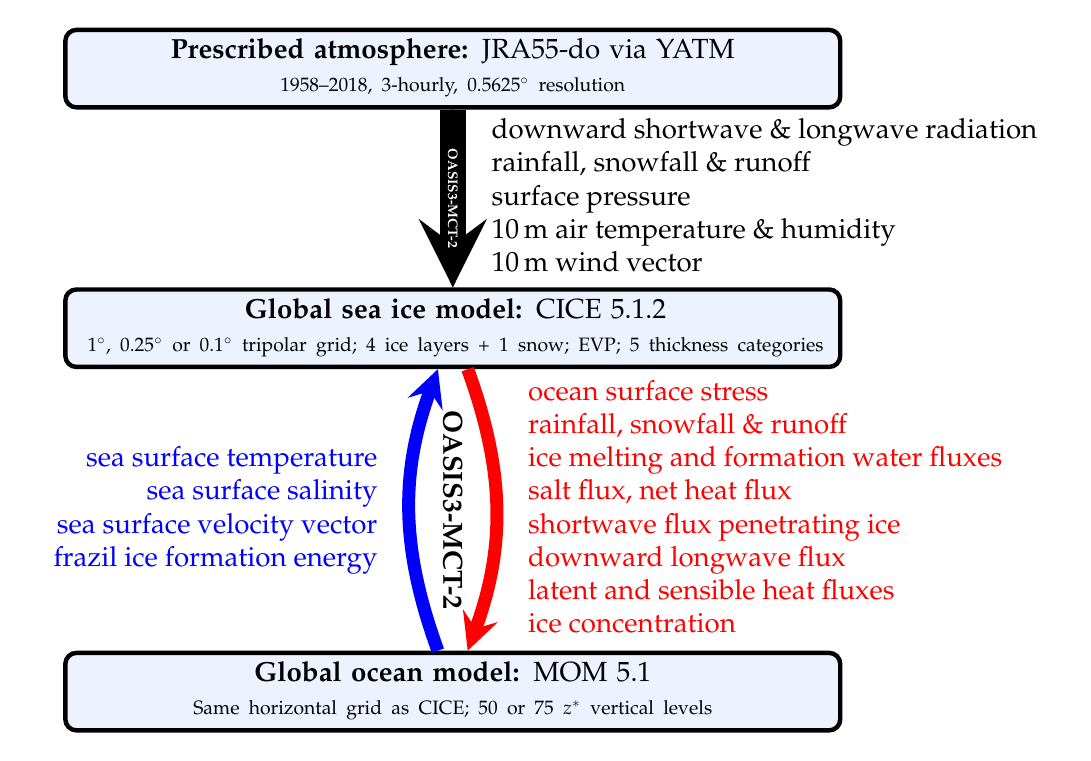
\begin{tikzpicture}[->,>=stealth,thick]
            
%             \node[state, text width=30ex] (ATM) 
             \node[state,
               text width=0.8\textwidth, 	% max text width
              fill=lightblue
               ] (ATM) 
            {\begin{tabular}{c}
              \textbf{Prescribed atmosphere:} JRA55-do %(Tsujino et al., 2018) 
              via YATM\\
    {\scriptsize1958--2018, 3-hourly, 0.5625$^\circ$ resolution}\\
%    {\scriptsize Climatological Antarctic runoff (Depoorter et al., 2013) at ice shelf edge}
              \end{tabular}};
              
             \node[state, 
              text width=0.8\textwidth, 	% max text width
              fill=lightblue,
              below of=ATM,
              node distance=20ex, %15ex,
              anchor=center] (ICE)
             {%
             \begin{tabular}{c}
              \textbf{Global sea ice model:} CICE 5.1.2\\
              {\scriptsize $1^\circ$, $0.25^\circ$ or $0.1^\circ$ tripolar grid; 4 ice layers + 1 snow; EVP; 5 thickness categories}
             \end{tabular}
             };
             
             \node[state,
              text width=0.8\textwidth, 	% max text width
              fill=lightblue,
             below of=ICE,
              node distance=28ex,
              anchor=center
              ] (OCEAN) 
             {%
             \begin{tabular}{c}
              \textbf{Global ocean model:} MOM 5.1\\
              {\scriptsize Same horizontal grid as CICE; 50 or 75 $z^*$ vertical levels}\\
%              {\scriptsize \textit{No ice shelf cavities, icebergs, distributed iceberg freshwater flux, tides, or waves (yet!)}}%, dynamic ice shelves
             \end{tabular}
             };
            
             \path 
%             (ATM) 	edge[line width=0ex] node[anchor=south,left]
%            {
%            \begin{tabular}{r}
%                downward shortwave \& longwave radiation\\
%                rainfall, snowfall, runoff, surface pressure\\
%%                10\,m air temperature \& humidity\\ % NB: namcouple comment is out of date - TsujinoETAL2018a state this is 10m (rather than 2m)
%%                10\,m wind vector
%            \end{tabular}
%            }
%                (ICE)
             (ATM) 	edge[line width=2ex] node[anchor=south,right]
            {
             \begin{tabular}{l}
                downward shortwave \& longwave radiation\\
                rainfall, snowfall \& runoff\\
                surface pressure\\
                10\,m air temperature \& humidity\\ % NB: namcouple comment is out of date - TsujinoETAL2018a state this is 10m (rather than 2m)
                10\,m wind vector
            \end{tabular}
            }
                (ICE)
             (ICE)  	edge[bend left=20, red, line width=1ex]                  node[anchor=left,right]
             {
            \begin{tabular}{l}
                ocean surface stress\\
                rainfall, snowfall \& runoff\\
                ice melting and formation water fluxes\\
                salt flux, net heat flux\\
                shortwave flux penetrating ice\\
                downward longwave flux\\
                latent and sensible heat fluxes\\
%                surface pressure\\  % passed to MOM but not used
                ice concentration
            \end{tabular}
            }
            (OCEAN)            
            (OCEAN)  	edge[bend left=20, blue, line width=1ex]  node[anchor=left,left]
             {
            \begin{tabular}{r}
                sea surface temperature\\
                sea surface salinity\\
                sea surface velocity vector\\
%                sea surface slope vector\\ % passed to CICE but not used: use_ocnslope=false
                frazil ice formation energy
            \end{tabular}
            }
            (ICE)
            (ICE)  	edge[bend left=0, white, line width=0ex]  node[sloped]
             {\textcolor{black}{\textbf{OASIS3-MCT-2}}}
            (OCEAN)
            (ATM)  	edge[bend left=0, black, line width=0ex]  node[sloped]
             {\textcolor{white}{{\tiny \textbf{OASIS3-MCT-2}}}}
            (ICE)
            ;
        
        \end{tikzpicture}
} 
\end{center}

    \caption[Coupling between model components.]{
    Coupling between model components by OASIS3-MCT-2 as specified in the \param{namcouple} file (which matches the atmosphere-CICE coupling fields specified in \paramsty{atmosphere/}\param{forcing.json} and the CICE-MOM coupling fields specified in \mom{mom_oasis3_interface_nml} in \paramsty{ocean/}\param{input.nml}).
    Notice that MOM receives atmospheric forcing via CICE rather than directly from YATM (CICE has the same global domain as MOM).
    Surface pressure is used in the surface fluxes routines in CICE to calculate the saturated vapour pressure.
    It is also passed from CICE to MOM, but we don't show it here because MOM ignores it in the current configuration since \mom{use_full_patm_for_sea_level}=false and  \mom{max_ice_thickness}=0. % https://arccss.slack.com/archives/C9Q7Y1400/p1549237452412700
    Similarly, the sea surface slope vector is passed from MOM to CICE but is unused (\cice{use_ocnslope} is false, so the sea surface slope is instead calculated from the sea surface velocity vector, assuming geostrophy) so is not shown here.
    Also see \url{https://github.com/COSIMA/access-om2/wiki/System-description}.
}
    \label{F:coupling}
\end{figure}

\begin{table}[tbp]
% update this with
%      cd namelists; python make_tables.py
\input{namelists/configurations.tex} 
\caption[Sources and paths to executables, inputs and outputs.]
{Sources and NCI paths to executables, inputs and outputs for the experiments in this document. 
These are based on the final run of each experiment; consult run summary spreadsheets for information on any changes within these experiments and details on computational resource use. 
Namelist changes within runs are tabulated in Appendix~\ref{S:namelist-diffs}.
Note that the last cycle of \param{1deg_jra55v13_iaf_spinup1_B1} was repeated with extra diagnostics in \param{1deg_jra55v13_iaf_spinup1_B1_lastcycle}.
The final source code and run configurations used here are at \url{https://doi.org/10.5281/zenodo.2653246} (or equivalently at \url{https://github.com/COSIMA/access-om2/releases/tag/GMD2019}).
The individual final run configurations are at
\url{https://github.com/COSIMA/1deg_jra55_iaf/releases/tag/1.0},
\url{https://github.com/COSIMA/025deg_jra55_iaf/releases/tag/1.0} and
\url{https://github.com/COSIMA/01deg_jra55_iaf/releases/tag/1.0}
}
\label{T:configs}
\end{table}

\pagebreak
\subsection{MOM configurations}

MOM parameters for the three model resolutions are tabulated in Appendix~\ref{S:mom-namelist}.
We discuss the choices of key parameters here.

The primary MOM5 reference is \citet{Griffies2012a}.  
\citet{GriffiesHarrisonPacanowskiRosati2008a} provides many useful technical details (despite being for MOM4).

The ocean formulation is hydrostatic and Boussinesq (volume-conserving), with a free surface and $z^*$ vertical coordinate.

The Boussinesq reference density is \mom{rho0} = \SI{1035.0}{kg m^{-3}}, the default value.

%Note hazards of tuning? \citet{DommengetRezny2018a}

%see /Users/andy/Documents/COSIMA/github/aekiss/namelist-check/namelist-meeting-2018-04-06/Fabio2018_Namelist_meeting.pdf

\subsubsection{Vertical grid}

The configurations use a $z^*$ vertical coordinate \citep[\mom{vertical_coordinate}='zstar'; ][section~5.1.4]{Griffies2012a}, with partial cells (see section~\ref{S:bathymetry}).
The vertical grid is staggered, with vertical velocity points offset from tracer points.
Vertical grid parameters are summarised in Tables~\ref{T:vgrid} and~\ref{T:access-om-ofam3-access-om2} and Figure~\ref{F:vgrid}.
The vertical grids are specified in the input file \param{ocean_vgrid.nc} for each configuration.
Vertical grid data is also available in the \param{ocean.nc} output files (see variables \param{st_ocean}, \param{st_edges_ocean}, \param{sw_ocean}, \param{sw_edges_ocean}).

%ACCESS-OM2 uses the same vertical grid as the ACCESS-CM2 coupled climate model, with 50 levels and 10.0\,m spacing in the top 200\,m, then increasing to 334.7\,m by the bottom at 6000\,m. % See Simon Marsland email 2018-12-03: ncdump -v st_edges_ocean /short/p66/dhb599/archive/bb039/history/ocn/ocean_month.nc-06751231 matches ncdump -v st_edges_ocean /g/data/hh5/tmp/cosima/access-om2/1deg_jra55v13_iaf_spinup1_A/output001/ocean/ocean.nc
%This is consistent past ACCESS-OM configurations, to maintain a baseline experiment against past tunings, et cetera.
%This grid differs from KDS50, GFDL50 and OFAM51 as defined by \citet{StewartHoggGriffiesHeerdegenWardSpenceEngland2017a}.
%Other configurations (not discussed here) use a modified KDS50 vertical grid for consistency with ACCESS-OM2-025.\TODO{check}
%\TODO{update for Abhi's new KDS50 run}

The vertical grids are optimised for resolving baroclinic modes \citep{StewartHoggGriffiesHeerdegenWardSpenceEngland2017a}.
The vertical grids in ACCESS-OM2 and ACCESS-OM2-025 are slightly modified versions of KDS50 \citep[][table~1]{StewartHoggGriffiesHeerdegenWardSpenceEngland2017a}, with 50 levels and 2.3\,m spacing at the surface, increasing smoothly to 219.6\,m by the bottom at 5363.5\,m.
%See email to Andy 1 Aug 2018 - IAF uses KDS50, whereas the RYF uses GFDL50? - no, now they are both KDS50
The vertical grid in ACCESS-OM2-01 is a slightly modified version of KDS75 \citep[][table~1]{StewartHoggGriffiesHeerdegenWardSpenceEngland2017a}, with 75 levels and 1.1\,m spacing at the surface, increasing smoothly to 198.4\,m by the bottom at 5808.7\,m.
The 75 level vertical grid is finer than OFAM3 at all depths other than 100 -- 260\,m and finer at all depths than GFDL50 and NEMO46 \citep[as defined by][]{StewartHoggGriffiesHeerdegenWardSpenceEngland2017a}.

\begin{table}
\newcolumntype{R}{>{\raggedleft\arraybackslash}p{12ex}}
\begin{tabularx}{\linewidth}{XRRRRR}
%\hline
%Model	 & 	$n$	&	$\Delta z_\text{min}$ (m)	& 	$\Delta z_\text{max}$ (m)	& 	$H_\text{max}$ (m)	\\
%\hline\endfirsthead
\hline
Model	 & 	$n$	&	$\Delta z_\text{min}$ (m)	& 	$\Delta z_\text{median}$ (m)	& 	$\Delta z_\text{max}$ (m)	& 	$H_\text{max}$ (m)	\\
\hline%\endhead
% from figures/grid/grid.ipynb
ACCESS-OM2 	&	 50 	&	 2.3	&	93.0	&	219.6	&	5363.5 \\
ACCESS-OM2-025 	&	 50 	&	 2.3	&	93.0	&	219.6	&	5363.5 \\
ACCESS-OM2-01 	&	 75 	&	 1.1	&	42.6	&	198.4	&	5808.7 \\
%ACCESS-OM2		&	50	&	10.0	&	334.7	&	6000.0\\	% ncdump -v st_edges_ocean /g/data/hh5/tmp/cosima/access-om2/1deg_jra55v13_iaf_spinup1_A/output001/ocean/ocean.nc
%ACCESS-OM2-025	&	50	&	2.3	&	219.6	&	5363.5\\	% ncdump -v st_edges_ocean /g/data/hh5/tmp/cosima/access-om2-025/025deg_jra55v13_iaf_gmredi/output001/ocean/ocean.nc
%ACCESS-OM2-01	&	75	&	1.1	&	198.4	&	5808.7\\	% ncdump -v st_edges_ocean /g/data/hh5/tmp/cosima/access-om2-01/01deg_jra55v13_iaf/output001/ocean/ocean.nc
\hline
\end{tabularx}
\caption[Vertical grid parameters.]{Vertical grid parameters: $n$ levels, with spacing of $\Delta z_\text{min}$ and $\Delta z_\text{max}$ at the surface and maximum depth $H_\text{max}$, respectively, and median spacing $\Delta z_\text{median}$.
Figure~\ref{F:vgrid} shows the distribution with depth.
\TODO{check that I'm correctly using the notation in \citet{StewartHoggGriffiesHeerdegenWardSpenceEngland2017a}}}
\label{T:vgrid}
%ncdump -v st_edges_ocean /g/data/hh5/tmp/cosima/access-om2/1deg_jra55v13_iaf_spinup1_A/output001/ocean/ocean.nc
% st_edges_ocean = 0, 10, 20, 30, 40, 50, 60, 70, 80, 90, 100, 110, 120, 130,
%    140, 150, 160, 170, 180, 190, 200, 210.923370361328, 229.097885131836,
%    261.064880371094, 312.015594482422, 385.282989501953, 482.015594482422,
%    601.064880371094, 739.097900390625, 890.923400878906, 1050,
%    1210.26977539062, 1372.68737792969, 1539.34790039062, 1712.24194335938,
%    1893.20642089844, 2083.87963867188, 2285.6611328125, 2499.67626953125,
%    2726.74975585938, 2967.38452148438, 3221.74975585938, 3489.67626953125,
%    3770.6611328125, 4063.87963867188, 4368.20654296875, 4682.24169921875,
%    5004.34814453125, 5332.6875, 5665.26953125, 6000 ;
%
%ncdump -v st_edges_ocean /g/data/hh5/tmp/cosima/access-om2-025/025deg_jra55v13_iaf_gmredi/output001/ocean/ocean.nc
% st_edges_ocean = 0, 2.30349978365172, 4.99384845577232, 8.13598848757999,
%    11.8057499021658, 16.0916668453325, 21.0970920758539, 26.9426551592365,
%    33.7691153258824, 41.7406645399246, 51.0487393569758, 61.9164000417828,
%    74.603329610196, 89.4114897901705, 106.691439004441, 126.849259570512,
%    150.353942802359, 177.744921530279, 209.639191756704, 246.737097161842,
%    289.82533120907, 339.775032772388, 397.532062043262, 464.095825684934,
%    540.482760486469, 627.671440120654, 726.529065262166, 837.724379025891,
%    961.639174086361, 1098.29705126241, 1247.32969180931, 1407.99436722564,
%    1579.24254229824, 1759.82425163261, 1948.40398485997, 2143.66476790834,
%    2344.38554694311, 2549.48748756835, 2758.05275811776, 2969.32320714254,
%    3182.68676319661, 3397.65794088943, 3613.85684298457, 3830.98925454079,
%    4048.82910238828, 4267.20370512379, 4485.9817563722, 4705.06374998657,
%    4924.37447144454, 5143.8571772085, 5363.46912067625 ;
%    
%ncdump -v st_edges_ocean /g/data/hh5/tmp/cosima/access-om2-01/01deg_jra55v13_iaf/output001/ocean/ocean.nc
% st_edges_ocean = 0, 1.08256153078322, 2.27890782887965, 3.60099746894928,
%    5.06204550134973, 6.67665534675832, 8.46096449334211, 10.4328054259553,
%    12.6118833596512, 15.0199725050152, 17.6811327608555, 20.6219489107565,
%    23.8717945936209, 27.4631235237192, 31.4317906511912, 35.8174061765097,
%    40.6637255570393, 46.0190788650439, 51.9368430613043, 58.4759609260126,
%    65.7015105143391, 73.68532905635, 82.506695148913, 92.2530728553569,
%    103.020920848004, 114.916568916192, 128.057162887489, 142.571677097719,
%    158.601990806908, 176.304021080078, 195.848899302919, 217.424171265553,
%    241.234991113943, 267.505266772175, 296.478698137217, 328.419628890149,
%    363.61360754513, 402.367523253464, 445.009148236631, 491.885882571281,
%    543.362462501468, 599.817368143857, 661.637658178801, 729.211984813624,
%    802.921613605928, 883.129411924441, 970.166985092353, 1064.32043027562,
%    1165.81551969179, 1274.80347061364, 1391.34871454206, 1515.42016508739,
%    1646.88730976903, 1785.52199214957, 1931.00606633608, 2082.94432975782,
%    2240.88143515938, 2404.32103311377, 2572.74526934082, 2745.63295762547,
%    2922.47517863585, 3102.78758377675, 3286.11918940845, 3472.05785157725,
%    3660.23287324829, 3850.31532207019, 4042.01665846308, 4235.08622153375,
%    4429.3080316501, 4624.49726832474, 4820.49668500234, 5017.17313981398,
%    5214.41435431341, 5412.12596212308, 5610.22887322482, 5808.6569552267 ;
\end{table}


\begin{figure}[htp]
\includegraphics[width=\textwidth]{figures/grid/vgrid.pdf}
\caption[Vertical grid spacing for the ACCESS-OM2 simulations.]{Vertical grid spacing for the ACCESS-OM2 simulations. 
ACCESS-OM2 and ACCESS-OM2-025 use the same vertical grid.
Left: the full depth range. 
Right: the upper ocean. 
The horizontal lines show the top and bottom of T cells.
Table~\ref{F:vgrid} provides further details.}
\label{F:vgrid}
\end{figure}

\pagebreak % try to avoid overrun
\subsubsection{Horizontal grid}\label{S:horizgrid}
% ncdump -h /short/v45/aek156/access-om2/input/mom_1deg/ocean_hgrid.nc
% ncdump -h /short/v45/aek156/access-om2/input/mom_025deg/ocean_hgrid.nc
% ncdump -h /short/v45/aek156/access-om2/input/mom_01deg/ocean_hgrid.nc

Grid parameters are summarised in Tables~\ref{T:hgrid} and~\ref{T:access-om-ofam3-access-om2}.
The horizontal grids are specified in the file \param{ocean_hgrid.nc} for each configuration.

In the horizontal, MOM and CICE use the same orthogonal curvilinear Arakawa B-grid with velocity components co-located at the northeast corner of tracer cells. 
Model configurations have been developed with zonal resolutions of 1$^\circ$, 0.25$^\circ$ and 0.1$^\circ$ south of 65$^\circ$N.
Figures~\ref{F:horizgrid}, \ref{F:horizgridNH} and~\ref{F:horizgridscatterhist} and Table~\ref{T:hgrid} show the grid spacing at the three resolutions.
Globally, the median cell size is 92\,km, 18.1\,km and 7.2\,km, respectively, at 1$^\circ$, 0.25$^\circ$ and 0.1$^\circ$ resolution.
Although the CICE model is global, the sea ice is mostly confined to latitudes higher than 60$^\circ$, where most cell dimensions are finer than 47.4\,km, 11.3\,km and 4.5\,km, respectively, at the three resolutions.

\begin{table}
\newcolumntype{R}{>{\raggedleft\arraybackslash}p{5.3ex}}
\begin{tabularx}{\linewidth}{|X|RRR|RRR|RRR|}
\hline
&\multicolumn{3}{c|}{Global} & \multicolumn{3}{c|}{North of 60$^\circ$N} & \multicolumn{3}{c|}{South of 60$^\circ$S}\\
& {\small min} & {\small median} & {\small max} & {\small min} & {\small median} & {\small max} & {\small min} & {\small median} & {\small max}\\
\hline
% from figures/grid/grid.ipynb:
{\small ACCESS-OM2 dx} &  23.8 & 91.7 & 111.2  &  24.7 & 32.7 & 54.8  &  23.8 & 43.0 & 54.6 \\
{\small ACCESS-OM2 dy} &  15.4 & 51.4 & 111.2  &  15.4 & 47.4 & 56.6  &  27.5 & 57.5 & 76.1 \\
{\small ACCESS-OM2 dx/dy} &  0.49 & 0.92 & 3.04  &  0.49 & 0.74 & 3.04  &  0.72 & 0.75 & 0.91 \\
\hline
{\small ACCESS-OM2-025 dx} &  6.0 & 18.1 & 27.8  &  6.2 & 8.1 & 13.9  &  6.0 & 11.3 & 13.9 \\
{\small ACCESS-OM2-025 dy} &  6.0 & 18.1 & 27.8  &  6.0 & 11.1 & 13.9  &  11.7 & 11.7 & 13.9 \\
{\small ACCESS-OM2-025 dx/dy} &  0.51 & 1.0 & 1.82  &  0.53 & 0.8 & 1.82  &  0.51 & 0.96 & 1.0 \\
\hline
{\small ACCESS-OM2-01 dx} &  2.19 & 7.16 & 11.12  &  2.47 & 3.29 & 5.55  &  2.19 & 4.52 & 5.55 \\
{\small ACCESS-OM2-01 dy} &  0.88 & 7.16 & 11.12  &  0.88 & 4.39 & 5.55  &  4.7 & 4.7 & 5.55 \\
{\small ACCESS-OM2-01 dx/dy} &  0.47 & 1.0 & 5.1  &  0.52 & 0.81 & 5.1  &  0.47 & 0.96 & 1.0 \\
\hline
\end{tabularx}
\caption[Statistics of ocean T-cell horizontal dimensions and aspect ratios.]{Statistics of ocean T-cell horizontal dimensions (in km) and aspect ratios; global distributions are shown in Figure~\ref{F:horizgridscatterhist}.}\label{T:hgrid}
\end{table}

The horizontal meshes are $360\times300$, $1440\times1080$ and $3600\times2700$ at 1$^\circ$, 0.25$^\circ$ and 0.1$^\circ$, respectively.
In all cases the grid covers the global ocean, extending from the North Pole to the Antarctic shelf edge but omitting the Antarctic landmass.
The T-grid extends to 
% these values are from yt_ocean
77.8766233766234$^\circ$S at 1$^\circ$,
81.0770008338366$^\circ$S at 0.25$^\circ$, and 
81.1297513555451$^\circ$S at 0.1$^\circ$.
The ocean extends to the southernmost cell at 1$^\circ$, but the other resolutions have a land mask covering the southernmost cells, giving southernmost ocean T-cell latitudes of
%77.87663$^\circ$S at 1$^\circ$,
78.22584$^\circ$S at 0.25$^\circ$, and 
79.58801$^\circ$S at 0.1$^\circ$.
% from geolat_t in ocean.grid.nc:
% -77.87663 in /g/data/hh5/tmp/cosima/access-om2/1deg_jra55v13_iaf_spinup1_B1/output059/ocean/ocean_grid.nc
% -78.22584 in /g/data/hh5/tmp/cosima/access-om2-025/025deg_jra55v13_iaf_gmredi6/output153/ocean/ocean_grid.nc
% -79.58801 in /g/data/hh5/tmp/cosima/access-om2-01/01deg_jra55v13_iaf/output197/ocean/ocean_grid.nc

The longitude range is $-280^\circ$E to $+80^\circ$E, placing the join in the middle of the Indian Ocean.
In all configurations the grid is tripolar \citep{Murray1996a} north of 65$^\circ$N (so the grid directions are not zonal and meridional in this region), with the tripoles placed on land at 65$^\circ$N, $-100^\circ$E and 65$^\circ$N, 80$^\circ$E. % see grid.ipynb
In the 0.25$^\circ$ and 0.1$^\circ$ configurations the grid is Mercator (i.e.\ the meridional spacing scales as the cosine of latitude) between 65$^\circ$N and 65$^\circ$S; south of 65$^\circ$S, the meridional grid spacing is held at the same value (in km) as at 65$^\circ$S.
The meridional variation of meridional grid spacing is more complicated in the 1$^\circ$ model (Figure~\ref{F:horizgridscatterhist}), and incorporates a refinement to 1/3$^\circ$ (of latitude) within 10$^\circ$ of the Equator \citep{BiMarslandUotilaOFarrellFiedlerSullivanGriffiesZhouHirst2013a, BiMarsland2010a}.

The 0.1$^\circ$ configuration had a misaligned CICE grid \WARNING in both the IAF run and the preceding RYF spinup --- see \url{https://github.com/COSIMA/access-om2/issues/190}.
%\url{https://github.com/mom-ocean/MOM5/blob/master/doc/web/user_guide.md}: ``The grid_spec file [/short/v45/aek156/access-om2/control/01deg_jra55_ryf] contains the following horizontal grid information: geographic location of T, E, C and N-cell (Tracer, East, Corner, and North cells), half and full cell lengths (in meters), rotation information between logical (i.e., grid oriented) and geographic east of cell. The complete description of the horizontal grid and namelist option is available in hgrid''

\TODO{maps of grid spacing divided by local 1st baroclinic Rossby radius from CheltonDeSzoekeSchlaxEl-NaggarSiwertz1998a \url{http://www-po.coas.oregonstate.edu/research/po/research/rossby_radius/index.html}?}

\begin{figure}[htp]
\includegraphics[width=\textwidth]{figures/grid/grid_1deg.png}\\
\includegraphics[width=\textwidth]{figures/grid/grid_025deg.png}\\
\includegraphics[width=\textwidth]{figures/grid/grid_01deg.png}
\caption{Horizontal grid spacing for the ACCESS-OM2 simulations. The colorbar limits show the minimum and maximum values. Note the meridional refinement near the equator in the 1$^\circ$ grid.
\TODO{also plot aspect ratio? see \citet{BiMarsland2010a}}}
\label{F:horizgrid}
\end{figure}

%\begin{figure}[htp]
%\includegraphics[width=\textwidth]{figures/grid/grid_scatter_1deg.png}\\
%\includegraphics[width=\textwidth]{figures/grid/grid_scatter_025deg.png}\\
%\includegraphics[width=\textwidth]{figures/grid/grid_scatter_01deg.png}
%\caption{Latitudinal variation of ocean T-cell dimensions in the ACCESS-OM2 simulations.}
%\label{F:horizgridscatter}
%\end{figure}
%
%\begin{figure}[htp]
%\includegraphics[width=\textwidth]{figures/grid/grid_hist_1deg.pdf}\\
%\includegraphics[width=\textwidth]{figures/grid/grid_hist_025deg.pdf}\\
%\includegraphics[width=\textwidth]{figures/grid/grid_hist_01deg.pdf}
%\caption{Cumulative histograms of horizontal grid spacing for ocean cells in the ACCESS-OM2 simulations.}
%\label{F:horizgridhist}
%\end{figure}

\begin{figure}[htp]
\includegraphics[width=0.32\textwidth]{figures/grid/NH_grid_1deg.png}\hfill
\includegraphics[width=0.32\textwidth]{figures/grid/NH_grid_025deg.png}\hfill
\includegraphics[width=0.32\textwidth]{figures/grid/NH_grid_01deg.png}
\caption{Land masks and T cell y-size in the Arctic tripolar region in the three resolutions.}
\label{F:horizgridNH}
\end{figure}


\begin{figure}[htp]
\includegraphics[width=.49\textwidth]{figures/grid/grid_scatter_1deg.png}\hfill
\includegraphics[width=.49\textwidth]{figures/grid/grid_hist_1deg.pdf}\\
\includegraphics[width=.49\textwidth]{figures/grid/grid_scatter_025deg.png}\hfill
\includegraphics[width=.49\textwidth]{figures/grid/grid_hist_025deg.pdf}\\
\includegraphics[width=.49\textwidth]{figures/grid/grid_scatter_01deg.png}\hfill
\includegraphics[width=.49\textwidth]{figures/grid/grid_hist_01deg.pdf}
\caption{Latitudinal variation of ocean cell dimensions (left), and cumulative histograms of horizontal grid spacing for ocean cells (right) in the ACCESS-OM2 simulations.
Table~\ref{T:hgrid} provides further statistics.}
\label{F:horizgridscatterhist}
\end{figure}

\subsubsection{Bathymetry}\label{S:bathymetry}
\CONTRIBUTORS{Russ Fiedler}

\begin{figure}[htp]
\includegraphics[width=\textwidth]{figures/bathymetry/partialcells.png}
\caption{Scatter plots of partial cell thickness versus full cell thickness in the three configurations. 
The upper and lower lines have slopes of 1 and 0.2, respectively.
For ACCESS-OM2-01 the cells are full-depth when thinner than 10\,m (i.e.\ the points fall on the upper line).}
\label{F:partialcells}
\end{figure}

Topography tools:

Various iterations of the 0.1$^\circ$ bathymetry are in 
\paramsty{/g/data/hh5/tmp/cosima/bathymetry}; see 
\paramsty{/g/data/hh5/tmp/cosima/bathymetry/README} and 
\paramsty{/short/v45/aek156/access-om2/input/mom_01deg/README-topog.txt} and 
\paramsty{/home/156/aek156/payu/01deg_jra55v13_ryf8485_spinup6/README-topog.txt}.

\param{kmt_min}: minimum number of vertical cells

The \param{topog.nc} seafloor topography (bathymetry) files were set up at each resolution with the help of \url{https://github.com/COSIMA/topogtools} and \url{https://github.com/mom-ocean/MOM5/blob/master/src/tools/make_topog/topog.c} and are read in by \url{https://github.com/mom-ocean/MOM5/blob/master/src/mom5/ocean_core/ocean_topog.F90} at runtime.
This reads \paramsty{work/ocean/INPUT/topog.nc} which points to \paramsty{/short/v45/aek156/access-om2/input/mom_01deg/topog.nc} - OR DOES IT?  This in turn is the same as \paramsty{/g/data/hh5/tmp/cosima/bathymetry/topog_13_06_2018.baffin.nc}.
At $0.1^\circ$ \paramsty{/short/v45/aek156/access-om2/control/01deg_jra55_iaf/config.yaml} specifies \paramsty{/short/public/access-om2/input_38570c62/mom_01deg/topog.nc}, which is the same as \paramsty{/g/data/hh5/tmp/cosima/bathymetry/topog_13_06_2018.baffin.nc}.
At $0.25^\circ$ the topography is specified in \paramsty{/home/157/amh157/payu/025deg_jra55_iaf_gmredi/config.yaml} as \paramsty{/g/data/ua8/MOM/grids/025/topog/KDS50/}
\TODO{what's the 1 deg topog?}
\FIXME{update all this}

The land mask in the two coarser resolutions was enlarged near the tripoles to remove small wet points, but this was not done at $0.1^\circ$ (figure~\ref{F:horizgridNH}).
Consequently the $0.1^\circ$ bathymetry retains the Gulf of Ob in Siberia and many channels in the Canadian Archipelago which are absent at coarser resolution.

There are no ice shelf cavities as these are not supported in MOM5.1. 

Mention the integrity checks and scripts used to generate the data (e.g. in \paramsty{/g/data/hh5/tmp/cosima/bathymetry/tools/common/}) --- should these be made publicly available? Also  \url{https://github.com/aekiss/notebooks/blob/master/non-advective.ipynb}.

%See figures/bathymetry/bathymetry.ipynb
The minimum depth is
45.11\,m (10 levels) in ACCESS-OM2,
40.36\,m (9 levels) in ACCESS-OM2-025, and
10.43\,m (7 levels) in ACCESS-OM2-01
--- see \url{}

\paragraph{1$^\circ$ and 0.25$^\circ$}
\WARNING The 1$^\circ$ and 0.25$^\circ$ topography files originate from the OCCAM model, from which they inherit a number of flaws such as anomalous `pits' on the shelves (for example excessive depth in the Gulf of Carpentaria and also the East Siberian and Chukchi seas south of Wrangel Island); see \url{https://github.com/mom-ocean/MOM5/issues/172}.
\WARNING They also have land masks that differ from each other and also from the 0.1$^\circ$ topography; see \url{https://github.com/COSIMA/access-om2/issues/158}.
%The minimum depths are 45.11\,m (10 levels) at 1$^\circ$, and 40.36\,m (9 levels) 0.25$^\circ$.
The 1$^\circ$ and 0.25$^\circ$ topography files were based on previously-generated files with the GFDL50 vertical grid and a (presumably 20\%) minimum partial cell thickness.
\WARNING When adapted to KDS50 the GFDL50 minimum cell thickness produces gaps in the thickness distribution (figure~\ref{F:partialcells}), i.e.\ the small terraces produced by the GFDL minimum partial cell thickness are inherited by the topography on the KDS50 vertical grid.
See \url{https://github.com/COSIMA/access-om2/issues/141}.

\paragraph{0.1$^\circ$}
The 0.1$^\circ$ bathymetry was generated from scratch by Russ Fiedler, and is therefore unaffected by the flaws that afflict the topography at 1$^\circ$ and 0.25$^\circ$.
It is based on GEBCO 2014 30 arcsecond gridded data % original data located at /g/data/hh5/tmp/cosima/bathymetry/gebco.nc
\FIXME{which version?} \url{http://www.gebco.net/data_and_products/gridded_bathymetry_data/gebco_30_second_grid/}
GEBCO is has 1\,m vertical resolution but this is averaged within each model grid cell, so the model topography is smoother (at least, before later processing).  
The topography data used in the runs is \paramsty{/short/v45/aek156/access-om2/input/mom_01deg/}\param{topog.nc}
also \paramsty{/g/data/hh5/tmp/cosima/bathymetry/}\param{topog_latest.nc}
\FIXME{update}

Topography ends at a vertical wall at the ice shelf edge (the calving line, not the grounding line).
A narrow strip along the southern boundary of the model is all land because the latitude range of the model was chosen for consistency with the previous MOM-SIS bathymetry which stopped at the grounding line. 

\TODO{plot or stats on how much model bathy differs from gebco}
plot bathymetry for the 3 resolutions -- incl difference from gebco and from 0.1deg as maps, scatter plots, histograms, and differences between the 3 resolutions, eg in Canadian archipelago

\TODO{mention main places where bathy tweaks were made -- see /g/data/hh5/tmp/cosima/bathymetry/README}

\paramsty{/g/data/hh5/tmp/cosima/bathymetry/README}: ``Enforced minimum of 7 levels (approx 10m). Excavated not filled in so land mask kept. Partial cells: Enforced thickness of max(10,0.2*dz). If partial cell were thinner than half this then the cell was removed.''

We use partial cells \citep{AdcroftHillMarshall1997a, PacanowskiGnanadesikan1998a} to obtain a more accurate representation of bottom topography.
%Partial cells in ACCESS-OM2-01:
%ncdump -h /short/v45/aek156/access-om2/input/mom_01deg/topog.nc
%yields 
%		depth:minimum_depth = 10.43281f ;
%		depth:minimum_levels = 7 ;
%		depth:min_thick = 10.f ;
%		depth:min_frac = 0.2f ;
%
%depth:min_thick=10m --- so there are no partial cells until the level thickness exceeds this.
For ACCESS-OM2-01 the minimum height of partial cells is 20\% of the full cell height, or $\min(10\,\text{m}, \Delta z)$, whichever is greater (depth:min_thick=10 in \param{topog.nc}; this modification is done by \url{https://github.com/mom-ocean/MOM5/blob/master/src/tools/make_topog/topog.c#L858}). 
\WARNING This means the minimum thickness is greater than 20\% of the full cell thickness if this is less than 50\,m (i.e.\ for depths shallower than 543\,m) and the cells are full-depth if they thinner than 10\,m  (i.e.\ for depths shallower than 103\,m) --- see figure~\ref{F:partialcells} and \url{https://github.com/COSIMA/access-om2/issues/99}). %See figures/bathymetry/bathymetry.ipynb
This produces terraces in shallow water.
This problem is fixed in more recent versions.

\subsubsection{Tracers}
\CONTRIBUTORS{Ryan Holmes}

At all three resolutions tracers (salt, temperature and age) are advected horizontally and vertically by the multidimensional piecewise parabolic method \citep{ColellaWoodward1984a}, with a monotonicity-preserving flux limiter following \citet{SureshHuynh1997a} (\param{horizontal-advection-scheme}=\param{vertical-advection-scheme}='mdppm' and \param{ppm_hlimiter}=\param{ppm_vlimiter}=3 for temp, salt and age in \paramsty{ocean/field_table}; also see \url{https://github.com/mom-ocean/MOM5/blob/master/src/mom5/ocean_tracers/ocean_tracer_advect.F90}).
\TODO{check: is this monotonicity-preserving under all conditions? \url{https://github.com/mom-ocean/MOM5/blob/99168b44ab45f4f5b4fa2544a0c3f644f0afb666/src/mom5/ocean_tracers/ocean_tracer_advect.F90}} % emailed Steve, 24 Mar 2019
%(Huynh, 1996)\TODO{find this and cite properly} 
% code has this citation but this doesn't contain a chapter by Huynh
%!<REFERENCE>
%! H.T. Huynh
%! Schemes and Constraints for advection
%! 15th Intern. Conf. on Numeric. Meth. in Fluid Mech., Springer (1997)
%!</REFERENCE>
%is it H. T. Huynh, Schemes and constraints for advection, in International Conference on Numerical Methods in Fluid Dynamics, Monterey, CA, 1996. ?
%https://www.springer.com/gp/book/9783662141151
%see https://ac.els-cdn.com/S0021999197957454/1-s2.0-S0021999197957454-main.pdf?_tid=87f51b89-5d2d-46d7-a4cf-08bf6df4274d&acdnat=1541380134_9213b4915ae345d204b79fe83ed07d08
As the $0.1^\circ$ configuration does not include a mesoscale eddy parameterization or explicit isopycnal or lateral diffusion (see section~\ref{S:subgridscalehoriz}), the suppression of large lateral tracer gradients near the grid-scale in this configuration is achieved solely though spurious numerical mixing in this tracer advection scheme.
\TODO{Reference to Holmes et al numerical mixing article/s}

\subsubsection{Sub-grid scale lateral / neutral physics}\label{S:subgridscalehoriz}
\CONTRIBUTORS{Ryan Holmes}

A sub-grid scale parameterization for mesoscale eddies is included in the $1^\circ$ and $0.25^\circ$ models (\mom{ocean_nphysics_nml} \param{use_this_module}=true), but not at $0.1^\circ$ as this resolution is considered ``eddy-resolving''. 
In the two coarser configurations the \citet{Gent1990} (GM) parameterization is used to represent the down-gradient isopycnal thickness flux associated with mesoscale eddies, and the along-isopycnal eddy tracer transport is parameterised by a Redi diffusivity \citep{Redi1982}. 
The namelist group \mom{ocean_nphysics_util_nml} controls these parameterisations; see \citet[][section~23.8]{Griffies2012a} for further explanation.
Note that the namelists are a bit confusing, as many ignored parameters are specified --- see \url{https://github.com/COSIMA/access-om2/issues/197}.
Their parameters are recalculated from scratch for each run, rather than being picked up from restarts  (\mom{nphysics_util_zero_init}=true).

The GM parameterization is implemented as a skew diffusive flux \citep{Griffies1998}.
In common with many GFDL configurations, we use the \param{ocean_nphysicsC} formulation (\mom{use_nphysicsc}=true) which differs from the default (\mom{use_nphysicsa}) in that the skew diffusive flux calculation is based on a vector streamfunction built from a sum of baroclinic modes.
% C is described as "experimental" but no longer is. 
% https://arccss.slack.com/archives/C6PP0GU9Y/p1572909972001700
% Russ Fiedler 2:12 PM 6 Nov 2019
% nphysicsC hasn't been experimental for a long, long time and nphysicsA hasn't been used in GFDL's configs for a while from what I can tell. nphysicsC is used in GFDL's ESM2M, and FLOR configurations at least. om3_core3 and the supplied MOM_SIS_TOPAZ used nphysicsB.
The associated diffusivity is depth-independent but flow-dependent (\mom{agm_closure}=true, \mom{agm_closure_baroclinic}=true), and is the product of \mom{agm_closure_scaling}, an inverse timescale, a squared length scale, and a grid scaling factor (see  \url{https://github.com/mom-ocean/MOM5/blob/4d60fad0e56/src/mom5/ocean_param/neutral/ocean_nphysics_util.F90#L2860}).
The length scale (\mom{agm_closure_length}) is 50\,km at  $1^\circ$ and 20\,km at $0.25^\circ$ (\mom{agm_closure_length} is used because \mom{agm_closure_baroclinic}=true --- see \url{https://github.com/mom-ocean/MOM5/blob/4d60fad0e5619fe15a630732ace4f0e3b3c6f23e/src/mom5/ocean_param/neutral/ocean_nphysics_util.F90#L2756}).
The inverse timescale is an Eady growth rate determined from the horizontal density gradient averaged between \mom{agm_closure_upper_depth}=100\,m and \mom{agm_closure_lower_depth}=2000\,m using a constant buoyancy frequency of \mom{agm_closure_buoy_freq}=\SI{0.004}{s^{-1}} (these three values are the defaults).
The Eady growth rate is subject to a limiter (\mom{agm_closure_eady_cap}) and is smoothed both vertically and horizontally (\mom{agm_closure_eady_smooth_horz}=true, \mom{agm_closure_eady_smooth_vert}=true) and vertically averaged in the mixed layer (\mom{agm_closure_eady_ave_mixed}=true).
The grid scaling (\mom{agm_closure_grid_scaling}=true) reduces the GM diffusivity in proportion to how well the numerical grid resolves the first baroclinic Rossby radius (or the equatorial Rossby radius within $\pm5^\circ$ latitude), as suggested by \citep{Hallberg2013a}.
The GM diffusivity is limited to the ranges 50--\SI{600}{m^2s^{-1}} at $1^\circ$ and 1--\SI{200}{m^2s^{-1}} at $0.25^\circ$ set by \mom{agm_closure_min} and \mom{agm_closure_max}.
It is not smoothed in space (\mom{agm_smooth_space}=false) or time (\mom{agm_smooth_time}=false).

The along-isopycnal Redi tracer diffusion \citep{Redi1982} in the two coarser configurations has a diffusivity that differs from GM (\mom{aredi_equal_agm}=false).
A constant coefficient of \mom{aredi}=\SI{600}{m^2s^{-1}} is used at $1^\circ$.
At $0.25^\circ$ the Redi coefficient is scaled by the resolution of the grid relative to either the first baroclinic Rossby radius, or the equatorial Rossby radius for latitudes between $\pm5^\circ$N (\mom{aredi_diffusivity_grid_scaling}=true), with a diffusivity no greater than \mom{aredi}= \SI{200}{m^2s^{-1}}.

\mom{drhodz_mom4p1} is true at $1^\circ$ but false at $0.25^\circ$.

Further testing of spatially- and temporally-dependent Redi and GM schemes has not yet been undertaken. 
However, given the sensitivity of the overturning circulation in the Southern Ocean and the formation of bottom water to the presence of these schemes exposed in a preliminary study in the $0.25^\circ$ configuration, such a sensitivity study should be high on the agenda.


All three configurations include a parameterization for re-stratification in the surface mixed layer due to submesoscale eddies \citep{Fox-Kemper2008}; see namelist group \mom{ocean_submesoscale_nml}. 
This parameterization applies an overturning circulation dependent on the horizontal buoyancy gradients within the mixed layer.
The optional horizontal diffusive portion of this parameterization is not used (\mom{submeso_diffusion}=false, so \mom{submeso_diffusion_biharmonic} and \mom{submeso_diffusion_scale} are ignored).

Horizontal friction is implemented with a biharmonic operator and an isotropic Smagorinsky scaling (\mom{k_smag_iso}=2.0, \mom{k_smag_aniso}=0.0) for the viscosity coefficient \citep{GriffiesHallberg2000a}; also see \citet[][chapter~25]{Griffies2012a}.
Our choice of \mom{k_smag_iso}=2.0 is below the lower limit of $\pi/\sqrt{2}\approx 2.2$ suggested by \cite{GriffiesHallberg2000a} and much less than the values of \mom{k_smag_iso}=3.0, \mom{k_smag_aniso}=3.0 used in OFAM3 (Appendix~\ref{S:ofam-namelist}), but matches what is used in ACCESS-CM2 (Appendix~\ref{S:OM2vsCM2}) and does not seem to cause numerical stability problems.
The $1^\circ$ configuration also has a grid spacing-dependent isotropic (\mom{vel_micom_aniso}=0.0) biharmonic background viscosity set by the velocity scale \mom{vel_micom_iso}=\SI{0.04}{m s^{-1}}; there is no background viscosity at the other resolutions.
The NCAR viscosity scheme is also applied at $1^\circ$ (\mom{ncar_boundary_scaling}=true), to enhance the background horizontal viscosity at western boundaries in order to ensure the western boundary currents are resolved (\mom{ncar_boundary_scaling}=true at 0.25$^\circ$ and 0.1$^\circ$ but this has no effect because \mom{vel_micom_iso} and \mom{vel_micom_aniso} are both zero).
%; see \param{ncar_*} in namelist group \mom{ocean_bihgen_friction_nml}.
%, and \paramsty{/short/public/access-om2/input_38570c62/mom_01deg/ncar_rescale.nc}. Or is this not being read? \mom{ncar_boundary_scaling_read} is false.
%This is set by \mom{ncar_boundary_scaling} in `MOM5/src/mom5/ocean_param/lateral/ocean_bihgen_friction.F90`
This increases the background viscosity at $1^\circ$ by a factor that is 4 on the i-maximum side of land cells at each depth, and decreases to 1 as a function of distance in the i direction (NB: this is not eastward distance in the tripole), with a profile that is a Gaussian with length scale \SI{500}{km} (the inverse of \mom{ncar_vconst_4} in cm), raised to the power \mom{ncar_rescale_power}=2.
\WARNING{The background viscosity is inconsistent along the tripole seam} with \mom{ncar_boundary_scaling}=true --- see \url{https://github.com/mom-ocean/MOM5/issues/282}.
At $1^\circ$ there is also background Laplacian viscosity at the bottom set by the velocity scale \mom{vel_micom_bottom}=\SI{0.01}{m s^{-1}} and calculated by a 5-point Laplacian operator (\mom{bottom_5point}=true).
The overall biharmonic viscosity is limited to \mom{visc_crit_scale}=25\% of the numerical instability threshold in ACCESS-OM2, or 100\% in the other two configurations \citep[see][equation (18.26)]{Griffies2004a}.
The Smagorinsky biharmonic viscosity $A_4$ varies spatially by orders of magnitude (Figure~\ref{F:viscosity}).
A viscous western boundary current has a width of about 3.6 times the length scale $(A_4/\beta)^{1/5}$ \citep[see][Appendix~B]{HaidvogelETAL92a}.
This thickness is about 350\,km in ACCESS-OM2, 100\,km in ACCESS-OM2-025, and 60\,km in ACCESS-OM2-01 (Figure~\ref{F:WBCwidth}), which is well-resolved by the grid in all cases.
The lateral boundary condition for velocity is no-slip, as a consequence of using a B-grid \citep{Griffies2012a}.
% we have \mom{use_side_drag_friction} unspecified and the default is false -- but this is for Deremble et al friction (law of the wall)

\begin{figure}[htbp]
\begin{center}
\includegraphics[width=.75\textwidth]{figures/viscosity/viscosity_EAC_clim.png}
\includegraphics[width=.75\textwidth]{figures/viscosity/viscosity_GulfStream_clim.png}
\includegraphics[width=.75\textwidth]{figures/viscosity/viscosity_Agulhas_clim.png}
\caption{Time-mean surface isotropic biharmonic viscosity $A_4$ in several western boundary regions.}
\label{F:viscosity}
\end{center}
\end{figure}

\begin{figure}[htbp]
\begin{center}
\includegraphics[width=.75\textwidth]{figures/viscosity/WBCwidth_EAC_clim.png}
\includegraphics[width=.75\textwidth]{figures/viscosity/WBCwidth_GulfStream_clim.png}
\includegraphics[width=.75\textwidth]{figures/viscosity/WBCwidth_Agulhas_clim.png}
\caption{Biharmonic western boundary current width $3.6(A_4/\beta)^{1/5}$ in several western boundary regions, based on the time-mean surface isotropic biharmonic viscosity $A_4$ (figure~\ref{F:viscosity}).}
\label{F:WBCwidth}
\end{center}
\end{figure}


\subsubsection{Sub-grid scale vertical physics}
\CONTRIBUTORS{Ryan Holmes}

Vertical diffusion of both tracers and momentum is parameterized using the K-profile parameterization \citep[KPP,][\mom{vert_mix_scheme}='kpp_mom4p1']{Large1994}, which governs mixing within the surface boundary layer, as well as interior convection (when the stratification is unstable), Richardson number-based shear instability (active mainly in the equatorial undercurrents), internal wave breaking, and double-diffusion.
\TODO{Comment on applicability of KPP at our high vertical resolution - see \citet{VanRoekelAdcroftDanabasogluGriffiesKauffmanLargeLevyReichlRingler2018a}}
KPP maintains static stability by applying large vertical diffusivity in regions with small or negative Richardson number; therefore explicit convective adjustment is not used at any resolution (see \mom{ocean_convect_nml}).
At $1^\circ$ the \citet{Jochum2009} latitudinally-dependent, depth-independent background vertical tracer diffusivity scheme is used (\mom{j09_diffusivity}=true), with diffusivity \mom{j09_bgmax}=\SI{5e-6}{m^2s^{-1}} poleward of \mom{j09_lat}=$\pm20^\circ$N, reducing to \mom{j09_bgmin}=\SI{1e-6}{m^2s^{-1}} at the equator via a cosine profile, similar to observations \citep{Gregg2003}.
The background vertical tracer diffusivity is zero in ACCESS-OM2-025 and ACCESS-OM2-01 (\mom{j09_diffusivity} is unspecified, and the default is false).
There is no additional non-tidal, non-KPP background vertical diffusivity at any resolution (\mom{background_diffusivity}=0.0).

There are no explicit tides, but we include vertical tracer diffusivity and vertical viscosity from parameterised internal and barotropic tidal processes. 
Turbulent mixing and viscosity due to breaking internal tides is parameterised by the \citet{SimmonsJayneLaurentWeaver2004a} scheme (\mom{use_wave_dissipation}=true) with a vertical decay scale \mom{decay_scale}=500\,m, zero background vertical diffusivity (\mom{background_diffusivity}=0.0), a constant background vertical viscosity of \mom{background_viscosity}=\SI{1e-4}{m^2s^{-1}}, tidal current speed read from the file \param{tideamp.nc} (\mom{read_tide_speed}) and bottom roughness amplitude read from the file \param{roughness_amp.nc} (\mom{read_roughness}=true and \mom{reading_roughness_amp}=true).
The \citet{LeeRosatiSpelman2006a} scheme is used to parameterise vertical mixing and viscosity due to the drag of barotropic tides on the bottom (\mom{use_drag_dissipation}).
Further parameters are in the \mom{ocean_vert_tidal_nml} namelist group.
\TODO{investigate whether newer dissipation estimates/methods should be used, e.g.\ are \citet{LavergneFalahatMadecRoquetNycanderVic2019a} and \url{https://doi.org/10.17882/58105} relevant?}

Bottom drag is calculated from the law of the wall using prescribed spatially-varying bottom roughness and tidal current speed (\mom{cdbot_roughness_uamp}=true), with residual current \mom{uresidual}=\SI{0.05}{m s^{-1}}.
Tidal current speed is read from the file \param{tideamp.nc} and bottom roughness is read from the file \param{roughness_cdbot.nc}.
The bottom drag coefficient is restricted to the range \mom{cdbot_lo} to \mom{cdbot_hi}, where \mom{cdbot_lo} takes its default value 0.001 and \mom{cdbot_hi}=0.007 (larger than the default value 0.003).
\mom{cdbot} is unused, since \mom{cdbot_law_of_wall}=false (the default).

The tidal speed data in \param{tideamp.nc} probably originates from \citet{JayneLaurent2001a} if it came from GFDL.\TODO{try to confirm this?} % from Russ https://arccss.slack.com/archives/C9Q7Y1400/p1554428974011900
The bottom roughness files seem basically the same, except that \param{roughness_amp.nc} is on T points and \param{roughness_cdbot.nc} is on U points.
They probably originate from \citet{JayneLaurent2001a} or \citet{Jayne2009a}, which in turn are derived from \citet{SmithSandwell1997a}.\TODO{try to confirm this?}% from Russ: https://arccss.slack.com/archives/C9Q7Y1400/p1541559974040600

\TODO{What is \param{drag_coeff} in \param{ocean_grid.nc}??}

\subsubsection{Rayleigh drag}\label{S:Rayleigh}
\index{Rayleigh drag}{Rayleigh drag} is a velocity tendency term proportional to the velocity, with a negative coefficient whose inverse magnitude is the $e$-folding time for velocity decay.
It is a momentum sink that is employed as an engineering fix to improve model stability and/or realism in a few selected locations in the $1^\circ$ and $0.1^\circ$ configurations, specified in \paramsty{ocean/}\param{field_table}, as shown in figure~\ref{F:Rayleigh}.
At $1^\circ$ it is used to improve the Indonesian Throughflow transport; a damping timescale of 1.5\,hr is applied at all but the bottom 2 (3) U-cells in Lombok (Ombai) Strait and for 3/4 of the width of the Torres Strait at all depths (\WARNING{these omissions were not intended}, and could be corrected in \paramsty{ocean/}\param{field_table} in new configurations: \url{https://github.com/COSIMA/access-om2/issues/156}).
At $0.1^\circ$ a damping timescale of 1.5\,hr is used at all depths across the full width of Kara Strait to constrain the velocity, which otherwise leads to numerical instability unless an unfeasibly small timestep is used.
There is no Rayleigh drag in the $0.25^\circ$ configuration.

\begin{figure}
\begin{center}
\includegraphics[height=0.3\textwidth]{figures/Rayleigh_drag/Rayleigh_undamped_cells_1deg.png}\quad
\includegraphics[height=0.3\textwidth]{figures/Rayleigh_drag/Rayleigh_undamped_cells_01deg.png}\\
\includegraphics[height=0.3\textwidth]{figures/Rayleigh_drag/Rayleigh_damp_time_1deg.png}\quad
\includegraphics[height=0.3\textwidth]{figures/Rayleigh_drag/Rayleigh_damp_time_01deg.png}
\end{center}
\caption[Rayleigh damping locations and magnitudes.]{
Rayleigh damping locations and magnitudes.
Circles indicate where Rayleigh damping is defined in \paramsty{ocean/}\param{field_table} and white cells are the U-grid land mask.
Top row: Rayleigh damping locations at $1^\circ$ (left; in the Lombok, Ombai and Torres Straits) and $0.1^\circ$ (right; in the Kara Strait); colours in the circled cells indicate how many U-cells are not damped in each column.
Bottom row: Rayleigh damping timescale (or zero if not defined) at $1^\circ$ (left) and $0.1^\circ$ (right). 
Where defined, damping timescales are all 5400\,s. 
There is no Rayleigh damping at $0.25^\circ$.
\label{F:Rayleigh}
}
\end{figure}

\subsubsection{Other model physical parameters}\label{S:otherparams}

\index{TEOS-10}We use the \citet{JackettMcDougallFeistelWrightGriffies2006a} pre-TEOS-10 seawater equation of state and freezing temperature (\mom{eos_preteos10}=true and \mom{freezing_temp_preteos10}=true).
The prognostic temperature variable is conservative temperature in the $1^\circ$ and $0.25^\circ$ configurations (\mom{temperature_variable}='conservative_temp'), and \WARNING potential temperature\footnote{This was an oversight: \url{https://github.com/COSIMA/access-om2/issues/97}, and has been corrected in the new $0.1^\circ$ RYF configuration, which uses conservative temperature: \url{https://github.com/COSIMA/access-om2/projects/1}.} in the $0.1^\circ$ configuration (\mom{temperature_variable}='potential_temp').
However \WARNING the $1^\circ$ and $0.25^\circ$ configurations mistakenly had \mom{pottemp_equal_contemp}=true, which meant that incorrect temperatures were passed to the coupler \url{https://github.com/COSIMA/access-om2/issues/148}.
The $0.1^\circ$ simulation also had \mom{pottemp_equal_contemp}=true, but the coupler fluxes are correct (since it used \mom{temperature_variable}='potential_temp') but \WARNING the conservative temperature output diagnostic is actually potential temperature.
Since we use pre-TEOS-10, practical salinity is the prognostic variable for salt for all the ACCESS-OM2 configurations (\url{https://github.com/mom-ocean/MOM5/blob/99168b44ab45f4f5b4fa2544a0c3f644f0afb666/src/mom5/ocean_core/ocean_density.F90#L209}).
If we switched to TEOS-10 \citep{RoquetMadecMcDougallBarker2015a} we'd need to use two salinity variables (Preformed Salinity and Absolute Salinity anomaly) instead of practical salinity: see \url{https://github.com/mom-ocean/MOM5/blob/99168b44ab45f4f5b4fa2544a0c3f644f0afb666/src/mom5/ocean_tracers/ocean_tempsalt.F90#L60} and \url{https://github.com/mom-ocean/MOM5/blob/99168b44ab45f4f5b4fa2544a0c3f644f0afb666/src/mom5/ocean_core/ocean_density.F90#L203} and \url{https://github.com/COSIMA/access-om2/issues/140}.
Frazil production is not confined to the top model layer (\mom{frazil_only_in_surface}=false) \TODO{check - ignored since we use auscom?}
and uses the pre-TEOS-10 freezing temperature (\mom{freezing_temp_preteos10})=true.

The Red Sea fix was not used (\mom{redsea_gulfbay_sfix}=false or unspecified).

Overflow schemes are not used (see \mom{ocean_overflow_nml} and \mom{ocean_overexchange_nml}).
Downslope transport and mixing schemes are only used at $1^\circ$, where we have sigma transport \citep{BeckmannDoscher1997a, CampinGoosse1999a, DoscherBeckmann2000a} with default parameters (\mom{ocean_sigma_transport_nml}) and downslope mixing (\mom{ocean_mixdownslope_nml}) with \mom{mixdownslope_npts}=4 (the default is 1).

Ice is massless / levitating (\mom{max_ice_thickness}=0) to avoid coupled ice-ocean instabilities \citep{Hallberg2014a}, but this alters the pressure applied to the ocean by the sea ice and precludes exact mass conservation in the coupled ocean and sea ice system (although mass is conserved within MOM5 itself, i.e.\ mass change rate equals net mass flux \TODO{strictly speaking, should "mass" be "volume"?}).
See \url{https://github.com/mom-ocean/MOM5/blob/7c8bb96/src/mom5/ocean_core/ocean_sbc.F90#L321}.
% see notes in `$ACCESS_OM_DIR/src/mom/src/mom5/ocean_core/ocean_sbc.F90`
We also have \mom{use_full_patm_for_sea_level}=false. In combination with \mom{max_ice_thickness}=0 this eliminates the inverse barometer and ice mass signals from eta_t:
\url{https://github.com/mom-ocean/MOM5/blob/ac2aeaab3753f1170f8dc9d1db4c7a5f3bbf7359/src/mom5/ocean_core/ocean_sbc.F90#L3936}
% see AK email to Griffies, 2018-08-16
%

\subsubsection{Timestepping}\label{S:timestepping}
The MOM baroclinic timestep is \accessom{ice_ocean_timestep} in \param{accessom2.nml}. %, overriding \mom{} in \param{input.nml}.
\accessom{ice_ocean_timestep} is also the CICE thermodynamic timestep, overriding \cice{dt} in \param{cice_in.nml}.
\accessom{ice_ocean_timestep} is chosen to be a factor of the JRA55-do forcing period of 3\,hr = 10800\,s, for example one of 100, 108, 120, 135, 144, 150, 180, 200, 216, 225, 240, 270, 300, 360, 400, 432, 450, 540, 600, 675, 720, 900, 1080, 1200, 1350, 1800, 2160, 2700, 3600 or 5400\,s.
Typical values are given in Table~\ref{T:ComputeResources}.
We use split timestepping, with the baroclinic timestep \mom{barotropic_split} = 80 times longer than the barotropic timestep.
Note that in going from baroclinic timestep $n$ to $n+1$ the barotropic solver integrates over a time interval covering baroclinic steps $n$ to $n+2$ in order to give a centred time-average at baroclinic step $n+1$; thus there are 160 times more barotropic timesteps than baroclinic timesteps \citep[][section~11.6]{Griffies2012a}.
% Note factor of two in \url{https://github.com/mom-ocean/MOM5/blob/99168b44ab45f4f5b4fa2544a0c3f644f0afb666/src/mom5/ocean_core/ocean_barotropic.F90#L1588}}
% but not in https://github.com/mom-ocean/MOM5/blob/3702ad86f9653f4e315b98613eb824a47d89cf00/src/mom5/ocean_core/ocean_model.F90#L943
% see https://arccss.slack.com/archives/C9Q7Y1400/p1549260376452300

The barotropic dynamics use a predictor-corrector method \citep[][sections~11.2.5 and~11.5]{Griffies2012a}, with the recommended method \citep[\mom{barotropic_time_stepping_a}=true; see][section~11.8.1]{Griffies2012a} and default dissipation parameter \mom{pred_corr_gamma}=0.2 and smoothing \mom{smooth_eta_t_laplacian}=true, \mom{vel_micom_lap}=\SI{0.05}{m s^{-1}}.
(\mom{smooth_eta_diag_laplacian} and \mom{smooth_pbot_t_laplacian} are ignored since we use a depth-based ($z^*$)  vertical coordinate, and
\mom{eta_max} and \mom{frac_crit_cell_height} are ignored because \mom{truncate_eta} is false.)

Two-level volume- and tracer-conserving timestepping schemes are used for the baroclinic dynamics (\mom{time_tendency}='twolevel'), with a staggered second-order forward method (tracer advection and lateral mixing of tracer and velocity calculated at timestep $n$ and pressure gradients calculated at timestep $n+\frac{1}{2}$ 
\TODO{check - see \citet[][chapter~11]{Griffies2012a}}%
% and https://github.com/mom-ocean/MOM5/blob/3702ad86f9653f4e315b98613eb824a47d89cf00/src/mom5/ocean_core/ocean_model.F90#L70
), implicit vertical mixing (\mom{aidif}=1.0) and bottom drag (\mom{bmf_implicit}=true), and semi-implicit Coriolis (\mom{acor}=0.5) calculations.
The tracer timestep is the same as the baroclinic dynamics timestep (\mom{baroclinic_split} = 1).
Velocity advection uses a second-order centred operator in space (\mom{velocity_advect_centered}=true by default) and third-order Adams-Bashforth timestepping (\mom{adams_bashforth_third}=true).
See \citet[][sections~11.3--11.6 and~11.8.1]{Griffies2012a}. 


\subsection{CICE sea ice model configurations}
The sea-ice component in the ACCESS-OM2 suite is based on CICE version 5.1.2 (\url{https://github.com/CICE-Consortium/CICE-svn-trunk/tree/cice-5.1.2}).
We have maintained our own fork at \url{https://github.com/COSIMA/cice5} which includes additional code such as the auscom drivers used in these runs.
We periodically update this fork to match the latest from the CICE consortium \url{https://github.com/CICE-Consortium/CICE-svn-trunk}.
The model runs reported here used commit 076b14f2 (table~\ref{T:configs}; \url{https://github.com/COSIMA/cice5/commit/076b14f2}) which was the 117th commit in our fork after an import of CICE 5.1.2 on 24 June 2015 (\url{https://github.com/COSIMA/cice5/commit/1110bae87}). % see \url{https://arccss.slack.com/archives/C9Q7Y1400/p1550192366062600}
Commit 076b14f2 did not include several bug fixes \WARNING which we have since imported from the CICE consortium (see commits cbf4c62 through to 320a796 at \url{https://github.com/COSIMA/cice5/commits/master}).
\TODO{check whether these bugs were relevant to our configs}

The primary CICE5 reference is \citet{HunkeLipscombTurnerJefferyElliott2015a-CICE5p1}.
CICE parameters for the three model resolutions are tabulated in Appendix~\ref{S:cice-namelist}; see \url{https://ncar.github.io/CICE/users_guide/ice_nml_var.html} for additional details.
We discuss the choices of key parameters here. 
The parameters are based on those of ACCESS-OM \TODO{check}  \citep{BiMarslandUotilaOFarrellFiedlerSullivanGriffiesZhouHirst2013a}, which used CICE4.1 and was the ocean-sea ice component of the ACCESS-CM coupled climate model \citep{BiDixMarslandOFarrellRashidUotilaHirstKowalczykGolebiewski2013a, DixVohralikBiRashidMarslandOFarrellUotilaHirstKowalczyk2013a}.
ACCESS-CM has now been superseded by ACCESS-CM2; CICE namelist differences between our ACCESS-OM2 1$^\circ$ configuration and ACCESS-CM2 are are tabulated in Appendix~\ref{S:cice-namelist-ACCESS-CM2-diff}.

CICE5 uses the same horizontal grid as MOM (see section~\ref{S:horizgrid}).
Its thermodynamic timestep is \accessom{ice_ocean_timestep}, the same as the MOM baroclinic timestep, but its dynamic and elastic timesteps are reduced by the factors \cice{ndtd} and \cice{ndte}$\times$\cice{ndtd} (respectively) as explained below.

\citet{BaileyETAL2018a}?

CICE parameter sensitivities: \citet{Hunke2010a}.

Parameter sensitivities: \citet{UotilaOFarrellMarslandBi2012a} found that sea ice volume and area are sensitive to albedo, snow patchiness, turning angle, ocean-ice heat transfer coefficient, and a ridging parameter. 
\citet{MillerLaxonFelthamCresswell2006a} documented a sensitivity of ice thickness, speed and extent to ice strength and the air-ice drag coefficient, whilst \citet{KimHunkeLipscomb2006a} found sensitivity of ice thickness to ice density, conductivity, maximum salinity, ice-ocean drag coefficient and ridging parameters. 
\citet{UrregoBlancoUrbanHunkeTurnerJeffery2016a} found a sensitivity to snow parameters and melt pond drainage.
Also see \citet{MassonnetGoosseFichefetCounillon2014a} (NEMO-LIM3).

cf. Andrew Roberts RASM cice namelist (Petra email 6 June) \TODO{get permisssion}
which was used in \citet{RobertsCraigMaslowskiOsinskiDuvivierHughesNijssenCassanoBrunke2015a, CassanoDuVivierRobertsHughesSeefeldtBrunkeCraigFiselGutowski2017a, HammanNijssenRobertsCraigMaslowskiOsinski2017a, JinDealMaslowskiMatraiRobertsOsinskiLeeFrantsElliott2018a, RobertsHunkeAllardBaileyCraigLemieuxTurner2018a}
see Appendix~\ref{S:rasm-namelist}

See Andrew Roberts' comments on \citet{RobertsCraigMaslowskiOsinskiDuvivierHughesNijssenCassanoBrunke2015a} in email from Petra email 6 June --- inertial coupling can be essential for stability

The CICE biogeochemistry code (group \cice{zbgc_nml}) is not used.

\subsubsection{Thickness redistribution}

We use 5 thickness categories (specified at compile time in build.sh by NICECAT).
We use \cice{kcatbound}=0, so the lower bound of ice categories is 0, 0.6445072, 1.391433, 2.470179 and 4.567288\,m (from \param{NCAT} in CICE output files), 
%0, 0.64, 1.39, 2.47, 4.57\,m 
as in \citet[][table 2]{HunkeLipscombTurnerJefferyElliott2015a-CICE5p1}.


We use the \citet{LipscombHunkeMaslowskiJakacki2007a} ridging scheme (\cice{krdg_partic}=1), with an $e$-folding scale parameter \cice{mu_rdg}=3\,m$^{1/2}$, which is the default value and matches ACCESS-CM2 (Appendix~\ref{S:cice-namelist-ACCESS-CM2-diff}) but is smaller than the value 2\,m$^{1/2}$ used in ACCESS-OM \citep[][table~2]{BiMarslandUotilaOFarrellFiedlerSullivanGriffiesZhouHirst2013a}.
\cice{maxraft} (the maximum thickness of rafted ice) takes the default value of 1.0\,m in ACCESS-OM2, ACCESS-OM and ACCESS-CM.

\subsubsection{Dynamics}\label{S:cicedynamics}
\TODO{check I (AK) haven't misunderstood anything here --- this is based on only a quick skim of most of these papers}

We are currently using ``classic EVP''
\footnote{
Another CICE option is the ``revised EVP'' method \citep[section~3.5.3]{BouillonFichefetLegatMadec2013a, HunkeLipscombTurnerJefferyElliott2015a-CICE5p1} which corrects an error in the ``classic EVP'' stress formulation and may also improve the convergence rate of the elastic sub-timesteps and reduce the incidence of spurious grid-aligned linear kinematic features (``leads'').
\TODO{try this out?}
\citet{BouillonFichefetLegatMadec2013a} argue that this is superior to using ``classic EVP'', but see warnings by \citet{KimmritzLoschDanilov2017a, KimmritzDanilovLosch2015a} that numerical instability may dominate over convergence as the greatest source of error.\FIXME{wrong references? they don't say this as far as I can see.}
}
 (\cice{kdyn}=1, \cice{revised_evp} = false) \citep{HunkeDukowicz1997a, HunkeDukowicz2002a, Hunke2001a}.
This represents the internal ice stresses by a visco-plastic (VP) rheology \citep{Hibler1979a}, to which a fictitious elastic term is added to facilitate efficient numerical convergence to the visco-plastic solution via damped elastic waves which are supposed to decay to negligible amplitude during \cice{ndte}=120 sub-timesteps within each dynamic timestep \citep[][sections~3.5.2 and~4.4; note that $\Delta t$ should be replaced by $\Delta t_\text{dyn}$ throughout section~3.5: see \url{https://github.com/CICE-Consortium/CICE/pull/83}]{HunkeLipscombTurnerJefferyElliott2015a-CICE5p1}.

There is an ongoing debate regarding the suitability of visco-plastic ice rheology, particularly to represent sea ice on fine scales \citep{Nye1973a, WeissSchulsonStern2007a, LindsayZhangRothrock2003a,KwokHunkeMaslowskiMenemenlisZhang2008a, GirardWeissMolinesBarnierBouillon2009a, DansereauWeissSaramitoLattes2016a, HutterLoschMenemenlis2018a, WeissDansereau2017a, HutterLoschMenemenlis2018a}. 
An alternative supported by CICE is the elastic-anisotropic-plastic (EAP) model \citep{WeissSchulson2009a, WilchinskyFeltham2006a, TsamadosFelthamWilchinsky2013a}, but this seems relatively untested and uncalibrated at this stage.

If we accept the VP formulation, there is also the question of how well the EVP sub-timesteping converges to the VP solution with no residual elastic wave effects.
Like many comparable models we use \cice{ndte}=120 sub-timestep iterations, but \citet{LoschDanilov2012a, LemieuxKnollTremblayHollandLosch2012a, KimmritzLoschDanilov2017a, KimmritzDanilovLosch2015a} show that full convergence may take thousands of iterations even with the revised EVP method (particularly at high resolution), which would be prohibitively expensive unless an accelerated method \citep[e.g.][]{KoldunovETAL2019a} was used. We must therefore expect our sea ice stress distribution to contain artefacts due to residual elastic waves. These artefacts may include spurious grid-scale noise and long linear features in the shear and divergence fields \citep{LemieuxKnollTremblayHollandLosch2012a}.
We note that the default \cice{ndte} has been increased to 240 in CICE6.

see \citet{LemieuxTremblay2009a}

Horizontal advection of conserved properties is handled by the incremental remapping scheme of \citet{DukowiczBaumgardner2000a} and \citet{LipscombHunke2004a}, documented in \citet[][section~3.2]{HunkeLipscombTurnerJefferyElliott2015a-CICE5p1}.
We find that the CFL condition associated with this method usually sets the maximum CICE dynamic timestep, which is shorter than the CICE thermodynamic timestep (and MOM baroclinic timestep) by the factor $\cice{ndtd}$.
This CFL condition becomes very restrictive at $0.1^\circ$ due to the very fine grid spacing in ocean cells near the tripole (table~\ref{T:hgrid} and figures~\ref{F:horizgrid} and~\ref{F:horizgridscatterhist}) so we set \cice{ndtd}=3 to allow MOM to run with a longer timestep.
We have not found this to be necessary in the coarser configurations, so these have \cice{ndtd}=1.
Using \cice{ndtd}=3 slows down CICE relative to MOM, altering the load balance.
We mitigate this by increasing the proportion of cores allocated to CICE in the  $0.1^\circ$ configuration (table~\ref{T:ComputeResources} and figure~\ref{F:scalingmomcice}) so that MOM does not spend so much time waiting for CICE, but this configuration still appears to be CICE-bound.
Newer configurations have greatly improved efficiency, partly by altering the bathymetry to eliminate the very smallest ocean cells.

%At 1$^\circ$ we have an ice-ocean turning angle of 16.26$^\circ$ \TODO{in which direction? presumably depends on hemisphere}(\cice{cosw}=0.96, \cice{sinw}=0.28) due to the 10\,m surface level thickness. 
In all three configurations the vertical grid resolution is fine enough to resolve the surface Ekman layer (Table~\ref{T:vgrid}), so we use a turning angle of zero (\cice{cosw}=1.0, \cice{sinw}=0.0), consistent with ACCESS-OM \citep[][table~2]{BiMarslandUotilaOFarrellFiedlerSullivanGriffiesZhouHirst2013a} and ACCESS-CM2 (appendix~\ref{S:cice-namelist-ACCESS-CM2-diff}; values unspecified but \cice{cosw}=1.0, \cice{sinw}=0.0 are the defaults).
(Is zero turning angle reasonable? see \citet{UotilaOFarrellMarslandBi2012a, ParkStewart2016a, McPhee2008a, Lepparanta2011a} --- we are using 10m ageostrophic winds and can resolve the ocean Ekman layer.)
% See emails 30 Nov 2018

We use an ice-ocean drag coefficient of \cice{dragio}=0.00536, consistent with ACCESS-OM \citep[][table~2]{BiMarslandUotilaOFarrellFiedlerSullivanGriffiesZhouHirst2013a} and very close to the value of 0.0054 measured at 0.5\,m below first-year landfast ice by \citet{ShirasawaIngram1997a}.
A wide range of values have been used in the literature \citep[][table~5.3]{LuLiChengLepparanta2011a, MartinsonWamser1990a, Lepparanta2011a}, but the coefficient also depends on the water velocity and depth at which it is measured, the ice roughness, and the upper ocean stratification \citep{Lepparanta2011a, WatersBruno1995a}.
Sensitivity to this parameter has been investigated by \citet{UotilaOFarrellMarslandBi2012a,UrregoBlancoUrbanHunkeTurnerJeffery2016a, KimHunkeLipscomb2006a}.

Sea ice drag coefficients and turning angles: \citet{HeortonTsamadosColeFerreiraBerbelliniFoxArmitage2019a}

\subsubsection{Thermodynamics}\label{S:cicethermo}


The albedo configuration is described in section~\ref{S:forcing}.

We use 4 ice layers and one snow layer (specified at compile time in build.sh by NICELYR and NSNWLYR, respectively).

We use the mushy ice formulation of \citet{TurnerHunkeBitz2013a} (\cice{ktherm}=2, \cice{tfrz_option}='mushy')  at 0.1$^\circ$.
At other resolutions we use the \citet{BitzLipscomb1999a} formulation (\cice{ktherm}=1, \cice{tfrz_option}='linear_salt').
In both cases the freezing point depends on salinity.
We also use a constant freezing temperature \cice{tocnfrz}=-1.8C --- should we switch to having a function of SSS that is consistent with \cice{tfrz_option}? --- see \citet{UotilaOFarrellMarslandBi2012a}.
These freezing points also differ from the frazil freezing point in MOM, for which we use \mom{freezing_temp_preteos10} = true.
See Andrew Roberts' comments on mushy thermo in email from Petra email 6 June 2018
``First, we are using mushy-layer thermodynamics, and
this needs to be carefully coupled so that the temperature in the ocean model's upper layer
matches the liquidus temperature in CICE, but the ocean model still conserves salt.''
\TODO{make freezing points consistent?}

We use the NCAR CCSM3 shortwave distribution method (\cice{shortwave}=`default'), which has implicit melt ponds.
Explicit melt ponds require the delta-Eddington radiation (\cice{shortwave}=`dEdd'), so the parameters in \cice{ponds_nml} are ignored in our configuration \TODO{check}.
See Andrew Roberts' comments on melt ponds in email from Petra email 6 June 2018.

Do we include lateral melting? see \cite{RoachDeanRenwick2018a}.

Consistent with ACCESS-OM \citep[][table~2]{BiMarslandUotilaOFarrellFiedlerSullivanGriffiesZhouHirst2013a}
we use the \citet{PringleEickenTrodahlBackstrom2007a} thermal conductivity parameterisation (\cice{conduct}='bubbly'), which improves the otherwise slow Antarctic ice growth rate \citep{Hunke2010a}, and an ice-ocean heat transfer coefficient of \cice{chio}=0.006 (\WARNING this is the value actually used, since the namelist value \cice{chio}=0.004 was ignored --- see \url{https://github.com/COSIMA/cice5/issues/55}) with minimum friction velocity \cice{ustar_min}=\SI{5e-3}{ms^{-1}}.


\subsection{Coupling}
See \url{https://github.com/COSIMA/access-om2/wiki/System-description}

Figure~\ref{F:coupling} shows the fields that are transferred between the coupled model components.
The prescribed atmosphere drives the global ice model, which is two-way coupled to the ocean model.
Coupling is implemented using the Ocean Atmosphere Sea Ice Soil \citep[OASIS3-MCT, ][]{ValckeCraigCoquart2013a} coupler version 2.0, developed at CERFACS and CNRS, France (\url{https://portal.enes.org/oasis}), which uses the Model Coupling Toolkit (MCT, \url{https://www.mcs.anl.gov/research/projects/mct/}) for routing between individual processors in each model component.
The OASIS3-MCT-2 user guide is here: \url{http://www.cerfacs.fr/oa4web/papers_oasis/oasis3mct_UserGuide_2.0.pdf}. 
The coupling strategy is based on the ACCESS-OM model \citep{BiMarsland2010a}, but we use a newer version of OASIS which is capable of parallel coupling.

The default remapping method used within OASIS3-MCT-2 (SCRIP \url{https://github.com/SCRIP-Project/SCRIP}) does not scale to 0.1$^\circ$. 
Instead the grid remapping interpolation weights are calculated using the RegridWeightGen application which is part of the ESMF framework \url{https://www.earthsystemcog.org/projects/esmf/}.
Conservative interpolation is used to remap flux fields (2nd order at 1$^\circ$ and 0.25$^\circ$, first order for 0.1$^\circ$: \url{https://github.com/COSIMA/access-om2/issues/71}).
For scalar fields we use a technique called patch recovery \citep{Kritsikis2017, Khoei2007} to produce very smooth destination fields. 
This is particularly important for the the 0.25$^\circ$ and 0.1$^\circ$ configurations because they have finer resolution than the forcing dataset. 
However the 2nd order conservative remapping method produces spurious extrema \WARNING (including nonsensical incorrect signs such as negative runoff or negative downwelling shortwave fluxes): \url{https://github.com/COSIMA/access-om2/issues/74#issuecomment-454660871}.
The creation of interpolation weights is documented at \url{https://github.com/COSIMA/access-om2/wiki/Technical-documentation#creating-remapping-weights}.

The atmosphere-to-ice coupling timestep is determined by the frequency of the atmospheric forcing dataset (i.e.\ 3 hourly for JRA55-do). 
Ice-to-ocean coupling takes place on every timestep (\accessom{ice_ocean_timestep}, the ocean baroclinic timestep and ice thermodynamic timestep), since \mom{baroclinic_split}=1.

%namcouple file list coupled fields
%
%atmosphere to ice: downward shortwave and longwave radiation, rainfall, snowfall, runoff, surface pressure, air temperature, humidity, 10m wind vector
%
%ice to atmosphere: 
%
%ice to ocean: stress vector, freshwater flux from rainfall and snowfall, runoff, salt flux, heat flux, shortwave flux penetrating ice, longwave flux, latent and sensible heat flux, surface pressure, ice concentration, ice melting and forming water fluxes
%
%ocean to ice: sea surface temperature, salinity, slope vector and velocity vector, frazil ice formation energy


\subsection{Forcing}\label{S:forcing}

There is no direct coupling from YATM to MOM5. Surface forcing is handled globally by CICE5, which obtains atmospheric data from YATM, interpolates it in time \TODO{check!}, and calculates various forcing fluxes to pass on to MOM5 via the OASIS3-MCT coupler (figure~\ref{F:coupling}).

The entire $0.1^\circ$ deg run was affected by a forcing bug: \WARNING \url{https://github.com/marshallward/payu/issues/138} and \url{https://github.com/COSIMA/access-om2/issues/123}.
The coarser model runs discussed here were not affected.

We have mass exchange of surface freshwater fluxes as in \citet{BiMarslandUotilaOFarrellFiedlerSullivanGriffiesZhouHirst2013a} \TODO{confirm}

JRA55-do v1.3 atmospheric forcing (1984-5, 1990-1 or 2003-4 repeat-year, 0.5625$^\circ$ ($\sim$55km), 3-hourly) in addition to CORE NYF (2$^\circ$ ($\sim$200\,km), 6-hourly)

JRA-55-do v1.3 forcing is supported at all three resolutions, and CORE2 forcing is supported at 1 degree resolution. 
JRA-55-do repeat-year forcing forcing (RYF) and interannual forcing (IAF)
% and CORE normal-year forcing (NYF) \FIXME{what about CORE IAF?}
are currently supported.

Ocean surface roughness following \citet{Beljaars1995a} % Beljaars (1994) in the code - presumably comments are wrong
(CICE parameter \cice{rough_scheme}=`beljaars`; note that this is also specified in MOM in \mom{ocean_rough_nml}, but this is for SIS and is therefore ignored).

The sea ice roughness \cice{iceruf}=\SI{5e-3}{m} matches that used in ACCESS-OM \citep[][table~2]{BiMarslandUotilaOFarrellFiedlerSullivanGriffiesZhouHirst2013a}.

Ocean albedo is constant (\cice{cst_ocn_albedo}=true), with the value \cice{ocn_albedo}=0.1, which is larger than the value 0.06 used in ACCESS-OM \citep{BiMarslandUotilaOFarrellFiedlerSullivanGriffiesZhouHirst2013a}.
(This has been changed to the \citet{LargeYeager2009a} latitude-dependent ocean albedo (\cice{cst_ocn_albedo}=false) in more recent versions.)
The MOM parameter \mom{ocean_albedo_option} is ignored.
In CICE5 we use the same NCAR CCSM3 shortwave distribution method (\cice{shortwave}=`default'),
ice and snow albedos in the visible ($\leq 700$\,nm) and infrared ($\geq 700$\,nm) bands
(\cice{albicev}, 
\cice{albicei}, 
\cice{albsnowv}, 
\cice{albsnowi})
and melt albedo parameters
(\cice{dalb_mlt} and 
\cice{ahmax})
\TODO{explain these}
as in ACCESS-OM \citep[][their table~2]{BiMarslandUotilaOFarrellFiedlerSullivanGriffiesZhouHirst2013a}, but we use the default snow patchiness parameter \cice{snowpatch} = 0.02\,m instead of the value 0.01\,m used in ACCESS-OM.
(We also set the same \cice{dt_mlt}=1.0$^\circ$C as ACCESS-OM but this Delta-Eddington parameter is ignored since \cice{shortwave}=`default'.)
The albedo parameters differ from those in \citet{HunkeLipscombTurnerJefferyElliott2015a-CICE5p1} and in JRA-55 \citep{KobayashiOtaHaradaEbitaMoriyaOnodaOnogiKamahoriKobayashi2015a}.
We use the default CCSM3 albedo type (\cice{albedo_type}='default'). \TODO{explain what this does}

Shortwave penetration into the ocean is handled by the GFDL scheme (\mom{ocean_shortwave_gfdl_nml}), with  \citet{ManizzaLe-QuereWatsonBuitenhuis2005a} optics (\mom{optics_manizza}=true).
The \citet{ManizzaLe-QuereWatsonBuitenhuis2005a} scheme splits the shortwave radiation flux equally into red and blue/green bands, and determines separate exponential decay scales for each band, with a term depending on chlorophyll-a concentration and a constant term for the absorption by pure seawater.
We use a prescribed monthly surface chlorophyll-a climatology (\mom{read_chl}=true) from the file \param{chl.nc}.
This climatology is based on SeaWiFS data from 1998--2006 \TODO{check: \citet[][sec~3.14.2]{Griffies2015a} says 1998--2007} and is presumably \TODO{check} the same as used in GFDL's CM2.5 and CM2.6 \citep{DelworthRosatiAndersonAdcroftBalajiBensonDixonGriffiesLee2012a, GriffiesWintonAndersonBensonDelworthDufourDunneGoddardMorrison2015a} based on the method of \citet{SweeneyGnanadesikanGriffiesHarrisonRosatiSamuels2005a}.
\WARNING The 0.25$^\circ$ and 0.1$^\circ$ \param{chl.nc} files have patches of missing data in the far north and south: \url{https://github.com/COSIMA/access-om2/issues/273}.
In the GFDL implementation this surface chlorophyll-a concentration is crudely approximated as independent of depth.
We also set a maximum penetration of \mom{zmax_pen}=\SI{300}{m}.
This limit is unlikely to have a noticeable effect, since even the slowest-decaying component (the blue/green band in clear water) has a decay scale $k=0.0232$\,m$^{-1}$, so the neglected fraction is at most $\frac{1}{2}\exp(-k$\,\mom{zmax_pen}$)=\SI{4.7e-4}{}$, and probably very much less.
 \TODO{set \mom{zmax_pen} to 1e6? see comments in code}

%, from \paramsty{/short/public/access-om2/input_38570c62/mom_01deg/chl.nc} at 0.1deg.

%% from Ryan:
%Shortwave radiation is distributed into the ocean interior using the scheme of \citet{ManizzaLe-QuereWatsonBuitenhuis2005a}, modulated by the climatological chlorophyll distribution compiled by \citet{SweeneyGnanadesikanGriffiesHarrisonRosatiSamuels2005a}.

There is no representation of geothermal heating (\mom{use_geothermal_heating}=false).
% https://arccss.slack.com/archives/C9Q7Y1400/p1541559974040600 Geothermal heating data - Russ is fairly sure it is this. Hamza, V., R. Cardoso, and C. F. Ponte Neto, 2008: Spherical harmonic analysis of the Earth's conductive heat flow. Int. J. Earth Sci., 97, 205-226,


\subsubsection{JRA55-do interannual and repeat-year forcing}

The ACCESS-OM2 configurations are forced with the JRA55-do v1.3 atmospheric reanalysis \citep[][and \url{http://www.cesm.ucar.edu/events/wg-meetings/2018/presentations/omwg/kim.pdf} and \url{https://climate.mri-jma.go.jp/~htsujino/jra55do.html}]{TsujinoETAL2018a} which has significantly improved bias, spatial and temporal resolution (55 km, 3-hourly), temporal extent (1958--2018), and dynamical self-consistency compared to the CORE dataset (200 km, 6-hourly, 1948--2009) used in many previous studies. We use recent calving and basal melt estimates from \citet{DepoorterBamberGriggsLenaertsLigtenbergBroekeMoholdt2013a}, which are spatially variable and somewhat larger than the uniform values in CORE \citep{TsujinoETAL2018a}. JRA55-do will also be regularly updated, allowing real-time experiments. The improved spatial resolution of wind is important for better representation of coastal polynyas \citep{StosselZhangVihma2011a, ZhangVihmaStosselUotila2015a}.
JRA55-do has higher spatial and temporal resolution and longer temporal extent than ERA-Interim (80\,km, 6-hourly, 1979--present) % https://www.ecmwf.int/en/forecasts/datasets/archive-datasets/reanalysis-datasets/era-interim
but is coarser and somewhat shorter than the upcoming ERA5 reanalysis (31\,km, 3-hourly, 1950--present): \url{https://confluence.ecmwf.int//pages/viewpage.action?pageId=74764925}.% https://www.ecmwf.int/en/forecasts/datasets/archive-datasets/reanalysis-datasets/era5

JRA55-do data are available from \url{https://esgf-node.llnl.gov/search/input4mips/?institution_id=MRI}.
It has been downloaded to NCI in a few places: 
\paramsty{/g/data/qv56/replicas/input4MIPs/CMIP6/OMIP/MRI/} (note that MRI-JRA55-do-1-3 is actually v1.3.1) and also
%\paramsty{/g/data/ua8/JRA55-do/RYF/v1-3/*.nc} or equivalently
\paramsty{/g/data/ua8/JRA55-do/v1-3} (note that 1-3 is actually 1.3.0; this is what was used for the ACCESS-OM2 v1.0 runs).
Also see \url{http://climate-cms.unsw.wikispaces.net/JRA55-do} and \url{https://github.com/COSIMA/access-om2/issues/120}.

The JRA55-do forcing file paths are constructed from the paths in \paramsty{atmosphere/}\param{forcing.json}, with \paramsty{INPUT} replaced by the paths in the atmosphere input section of \param{config.yaml} and \paramsty{\{\{year\}\}} replaced by the model years over the range set in \param{accessom2.nml}.
%The actual JRA55-do forcing files that are read are listed in \param{manifests/input.yaml}.

See JRA55_RYF_justification.ipynb for biases in each RYF year.

JRA55-do \citep{TsujinoETAL2018a} is a surface-atmospheric reanalysis product derived from the 55-year Japanese reanalysis (JRA55, \url{http://jra.kishou.go.jp/JRA-55/index_en.html}) and intended for driving oceans models. 
We use JRA55-do version 1.3 to drive our ice and ocean models.
The temporal coverage is from 1st January 1958 to 1st February 2018, but it is regularly updated to near present day.

JRA55-do v1.3 user manual: \citet{TsujinoUrakawaNakanoSmallKimYeagerDanabasogluSuzukiBamber2018a}

For the latest information on the dataset status and citation: \url{http://goo.gl/r8up31}.

see \url{http://amaterasu.ees.hokudai.ac.jp/~tsujino/JRA55-do-v1.3/00README_v1_3.1st}
JRA-55: \citet{KobayashiOtaHaradaEbitaMoriyaOnodaOnogiKamahoriKobayashi2015a}
JRA55-do: \citet{Tsujino2015a, Tsujino2015b, Tsujino2016a, TsujinoETAL2018a}, \citet{TsujinoUrakawaSuzukiKomuroSmallKimYeagerDanabasogluGriffies2016a},
\citet{KimSmallYeagerDanabasogluTsujinoETAL2018a}


\url{http://www.clivar.org/omdp/japan2016}

JRA55-do version 1.3 provides
3-hourly liquid and solid precipitation, downwelling surface longwave and shortwave radiation, sea level pressure, 10m wind velocity components, 10m specific humidity and 10m air temperature \citep[NB: humidity and temperature are shifted from 2m in JRA55 to 10m in JRA55-do --- see][, appendix A2]{TsujinoETAL2018a}
on a TL319 grid (0.5625$^\circ$ resolution), and daily river flux at 0.25$^\circ$ resolution.

\TODO{check: what do we use for glacier runoff? groundwater? evaporation? upwelling longwave radiation?}

``Runoff from Greenland and Antarctica are replaced by climatological runoff.
Greenland runoff is based on \citet{BamberBroekeEttemaLenaertsRignot2012a} and Antarctica runoff
is based on \citet{DepoorterBamberGriggsLenaertsLigtenbergBroekeMoholdt2013a}.'' (\url{http://amaterasu.ees.hokudai.ac.jp/~tsujino/JRA55-do-v1.3/00README_v1_3.1st})

The Antarctic runoff is spatially variable in JRA55-do \citep{TsujinoETAL2018a}, in contrast to CORE .

we made a start on this: \url{https://github.com/COSIMA/matm/issues/5}

%should we / do we use this for runoff? \citet{SuzukiYamazakiTsujinoKomuroNakanoUrakawa2018a}

currently fresh water is input at the ice shelf edges.

cf.\ runoff (iceberg discharge scheme) used in ACCESS-CM2 - see AMOS2018 notes on Dave Bi's talk and \url{https://accessdev.nci.org.au/trac/wiki/CMIP6workshop}
--- this is discharged only at the surface.
See Siobhan's email 2018-06-04

Runoff - incl distributed iceberg melt? Ask Adele? basal melt needs to be at depth - notebook p561, \citet{MathiotJenkinsHarrisMadec2017a}. We have the data but waiting on it being published. 
Veronique has regridded this - see email 2017-11-16 \citet{MerinoLeSommerDurandJourdainMadecMathiotTournadre2016a} and
\citet{DepoorterBamberGriggsLenaertsLigtenbergBroekeMoholdt2013a}
Paul: ``The Antarctic ice berg data is published and the data is publicly available here: 
\url{http://neichin.github.io/personalweb/publications/}
However, the Antarctic basal melt fluxes are not published yet and the data has not been made public.''
Also see \citet{MerinoJourdainLe-SommerGoosseMathiotDurand2018a, Donat-MagninJourdainSpenceLe-SommerGalleeDurand2017a, MathiotJenkinsHarrisMadec2017a,HammondJones2016a, StosselNotzHaumannHaakJungclausMikolajewicz2015a}

JRA55-do river runoff is from \citet{SuzukiYamazakiTsujinoKomuroNakanoUrakawa2018a}; this is daily, interannually varying runoff from the JRA55 land surface model at 0.25$^\circ$ resolution, adjusted to match the observational estimates of \citet{DaiQianTrenberthMilliman2009a}.
River runoff is combined with climatological monthly solid runoff for Greenland \citep{BamberBroekeEttemaLenaertsRignot2012a} and spatially-variable annual mean climatological basal melt and calving from Antarctica \citep{DepoorterBamberGriggsLenaertsLigtenbergBroekeMoholdt2013a}.
Calving and liquid runoff are combined (\mom{discharge_combine_runoff_calve} defaults to true). 
River discharge is inserted at the coast in the top \mom{river_insertion_thickness}=40\,m, but other runoff is inserted only at the surface (\mom{runoff_insertion_thickness} and \mom{calving_insertion_thickness} default to zero) at the ice shelf edge.
Total runoff is remapped (and spread horizontally if needed to keep the flux below a threshold) in real time by YATM --- see section~\ref{S:YATM}.

runoff tools: \url{https://github.com/COSIMA/runoff_tools}

RYF: cite \citep{StewartKimUrakawaHoggYeagerTsujinoNakanoKissDanabasoglu2020a}; cf.\ \citet{Roske2006a}.

discuss choice of year for RYF --- will use 1984-5 for high-res runs -- refer to Kial's paper

RYF generated by \url{https://github.com/aidanheerdegen/make_ryf}.

These 12-month periods were identified as particularly "neutral":
1 May 1984 - 30 April 1985,
1 May 1990 - 30 April 1991,
1 May 2003 - 29 April 2004 (we keep 29 Feb 2004 and ditch 30 April 2004 so as to keep 365 days per year).
We have run ocean-sea ice spinups forced by all three JRA55-do v1.3 repeat years at 1$^\circ$ but we are concentrating on 1984-5 for the 0.1$^\circ$ spinup as it has less of the warming signal and also gives us more of the JRA55 dataset for subsequent interannual runs.

Kial's email 2018-03-05:
\begin{quote}
-1st of January is in the peak of the northern winter and southern summer, meaning the variability in forcing fields (ie. weather) is quite high. This is a problem for surface buoyancy fluxes in the north Atlantic and Labrador \& Nordic Sea regions, where NADW formation is notoriously sensitive to changes in surface forcing. The day of the year with lowest variability (least weather) is going to be closer to the equinoxes, and in JRA55 DO it turns out to be 1 May. 

-The three candidate years have been selected as the 12-month periods with climate indices closest to neutral. The climate indices of interest are the SOI, SAM and NAO. Removing the criteria that a 12-month period follows the calendar year allows us to find "years" that are closer to climatologically neutral.

-Having the jump at 1 May allows us to run the model harder. The model tends to fall over at 1 Jan if the jump is there, meaning we have to back off the timestep and nurse it through. Having the jump at 1 May does not require any such nursing. Currently we are running the ACCESS-OM2 1$^\circ$ with 5400 sec timesteps from initialization and getting through ~90 years per day.
\end{quote}
\TODO{plots of anomalies from climatology for the time-mean (or seasonal-mean) RYF forcing fields}


see \url{https://github.com/COSIMA/access-om2/issues/52} and \url{http://www.earthsystemmodeling.org/esmf_releases/last_built/ESMF_refdoc/node3.html#SECTION03020000000000000000}

All versions of JRA55-do up to and including v1.4.1 had some tropical cyclones in the Northeast Pacific \WARNING and the North Atlantic from 1959 to 1987 erroneously represented as anti-cyclonic vortices: \url{https://github.com/COSIMA/access-om2/issues/186}.
RYF8485 (1 May 1984 - 30 April 1985) has four faulty North Atlantic storms but RYF9091 and RYF0304 are OK.
This issue is fixed in JRA55-do v1.5.

SST suddenly gets worse at end of 1990's at all resolutions, and stays that way \citep[][figure 3b]{KissETAL2020a} --- is there a persistent problem with JRA55-do? Or is it just that the 18$^\circ$C offset is wrong?

%\subsubsection{CORE-NYF}
%\url{http://www.clivar.org/clivar-panels/omdp/core-2}
%2$^\circ$, 6-hourly

The new IAF configuration will use JRA55-do 1.4.0 from
\paramsty{/g/data/qv56/replicas/input4MIPs/CMIP6/OMIP/MRI/MRI-JRA55-do-1-4-0}.
At present this extends to 5 Jan 2019, which is as much as is currently available from
\url{https://esgf-node.llnl.gov/search/input4mips/}
but this will be extended close to the present day from time to time --- e.g. there is a beta version v1.4.0.1beta extending to 11 Jan 2020:
\url{https://climate.mri-jma.go.jp/~htsujino/jra55do.html}.
The JRA55-do v1.4.0 user manual is here: \url{https://climate.mri-jma.go.jp/~htsujino/docs/JRA55-do/v1_4-manual/User_manual_jra55_do_v1_4.pdf} \citep{TsujinoETAL2019a}.

\subsubsection{Restoring}\label{S:restoring}

The only restoring we apply is to surface salinity.
This is restored to interpolated \TODO{state interpolation method --- Smoothing at 0.1deg to deal with spurious discontinuities and noise in WOA13v2: \url{https://github.com/COSIMA/access-om2/issues/103}} World Ocean Atlas 2013 v2 monthly climatology (\url{https://www.nodc.noaa.gov/OC5/woa13/}); the interpolated salinity file is \param{salt_sfc_restore.nc}. % ncdump -h salt_sfc_restore.nc gives: This salinity distribution is based on WOA13v2 where the land values are filled in with a conjugate gradient method. It is a simple average of land-filled salinity data at the depth of 0 and 10 meters.
The restoring timescale is set by \mom{salt_restore_tscale}; we use 10 days at 0.1$^\circ$ and 21.28 days for the coarser resolutions.
The ``piston velocity`` (surface vertical grid spacing divided by restoring timescale) is more physically relevant than the restoring timescale.
This is 0.11\,m/day at all resolutions due to the differing vertical resolution (see Table~\ref{T:vgrid}).
This piston velocity is within the range of values used for CORE-II models, but is somewhat weaker restoring than the 50\,m/300\,days (i.e.\ 0.167\,m/day) used for GFDL's MOM simulations \citep[][table~2]{DanabasogluETAL2014a}.
%For comparison, 15\,m/300\,days (i.e.\ 0.05\,m/day) is GFDL's standard piston velocity (Griffies, 12 April 2018), so we are restoring about twice as strongly as GFDL. % must have misheard 50 as 15, since 15 is inconsistent with 50m/300days in table 2 of DanabasogluETAL2014a

We apply salinity restoring via a salt flux (\mom{use_waterflux} =  true, \mom{salt_restore_as_salt_flux} = true) and restore everywhere, including under ice (\mom{salt_restore_under_ice} = true).
A spatially constant offset is added to the salt restoring to ensure that the net salt restoring flux is zero for each timestep (\mom{zero_net_salt_restore} = true).
In order to avoid excessively large fluxes the SSS mismatch is limited to \mom{max_delta_salinity_restore} = 0.5\,psu for the purposes of calculating the restoring flux at 0.25$^\circ$ and 0.1$^\circ$ (but not at 1$^\circ$).
We don't use \mom{salinity_restore_limit_lower} or \mom{salinity_restore_limit_upper}, so \mom{max_delta_salinity_restore} applies even in regions of extremely low or high salinity (see \url{https://github.com/mom-ocean/MOM5/issues/203}).

We close the water budget by imposing a constraint of zero net water flux into the combined ocean-sea ice system from the coupler (\mom{zero_net_water_coupler} = true) by removing the area-mean of $P-E+R$ (precipitation - evaporation + runoff) from $P-E$ (also adjusting \param{liquid_precip} for consistency) so that the area-integrated $P-E+R=0$ at each timestep; this does not constrain water exchanges with the sea ice (see section~\ref{S:oceanvol}).
%\FIXME{how does this work, given that some of the precip falls as snow on ice to be released later, but \mom{zero_net_water_coupler} is a MOM thing? see \url{https://arccss.slack.com/archives/C9Q7Y1400/p1572993155004300}}
%\mom{zero_net_water_restore} = true.
Note that the MOM diagnostics \param{pme_river} and \param{total_pme_river} report the water fluxes into the ocean model component (not the total ocean-sea ice system), so are non-zero due to water exchange with sea ice due to freezing and melting.
See these code sections for
\href{https://github.com/mom-ocean/MOM5/blob/730f0bf56f64fad0d9abcfa973b7348a89c175c3/src/mom5/ocean_core/ocean_sbc.F90#L231-L243}{documentation on \param{zero_net_water_coupler}},
\href{https://github.com/mom-ocean/MOM5/blob/730f0bf56f64fad0d9abcfa973b7348a89c175c3/src/mom5/ocean_core/ocean_sbc.F90#L3638-L3646}{addition of ice melt to \param{pme}},
\href{https://github.com/mom-ocean/MOM5/blob/730f0bf56f64fad0d9abcfa973b7348a89c175c3/src/mom5/ocean_core/ocean_sbc.F90#L4014-L4078}{adjustment to ensure zero water flux},
and output of
\href{https://github.com/mom-ocean/MOM5/blob/730f0bf56f64fad0d9abcfa973b7348a89c175c3/src/mom5/ocean_core/ocean_sbc.F90#L5942}{\param{pme_river}} and
\href{https://github.com/mom-ocean/MOM5/blob/730f0bf56f64fad0d9abcfa973b7348a89c175c3/src/mom5/ocean_core/ocean_sbc.F90#L5953}{\param{total_pme_river}} diagnostics.

These salt restoring and freshwater parameter choices are typical of CORE-II models \citep[][table~2]{DanabasogluETAL2014a}.

%https://arccss.slack.com/archives/C9Q7Y1400/p1572993155004300
%aekiss 9:32 AM, 6 Nov 2019
%Hi @Russ Fiedler I've added this text to the access-om2 paper:
%We impose a constraint of zero net water flux into the ice-ocean system from the coupler, by removing the area-mean of precipitation $P$ minus evaporation $E$ plus runoff $R$ from $P-E$ so that the integrated $P-E+R$ is zero at each timestep; this does not constrain water exchanges between the ocean and sea ice.
%is this a correct description of the effect of zero_net_water_coupler=true, in particular that it constrains flux to the ice-ocean system?
%I'm a bit confused, as the description in the code initially says it sets zero net flux into the ocean (rather than ocean+ice): https://github.com/mom-ocean/MOM5/blob/f160f805260b2735ce1695095c0c6d4e18dd2281/src/mom5/ocean_core/ocean_sbc.F90#L231
%Russ Fiedler 10:44 AM
%Yes, it's just the ocean component that's being constrained at each time step. There's obviously rain/snow on ice and evaporation there and can fluctuate however in the long term it gets zeroed out. The trick is the "melt" term which is proportional to the salt exchange between ocean/ice.
%aekiss 12:27 PM
%Thanks but I'm still confused. Do you mean that the total water in the ice+ocean system can vary because there can be a net E-P+R over ice? I don't understand how melt could fix this, since the melt term doesn't alter the total water in the ice+ocean system. And if E-P+R>0 over ice, won't this go into snow, which has no associated salt flux when it melts? Revealing my ignorance here!
%Russ Fiedler 1:39 PM
%Yes, that's right. There's a net P-E over ice. But this eventually goes into P between ice/ocean and gets zeroed out in the long run.
%andy 9:39 PM
%OK, I�m not convinced by this. I can see from the code that pme+river is balanced by zero_net_water_coupler. And I can see ice which is formed and then one day melts again will get zeroed out in the long run. But I can�t see what happens to precip which lands on the sea ice (as snow or water). Is this passed into the ocean as melt or as precip? If the former, then how can it be balanced? If the latter, I can�t see how that is achieved �
%Russ Fiedler 11:01 AM Nov 7 2019
%It gets  passed as precip. melt is calculated via the salt exchange. It's both positive and negative. Consider a cycle of ice formation and complete melting. The pme contribution is zero all the time and if salt is conserved across the ocean ice interface then the melt contribution should be zero as you mention. In practice,  if starting with zero ice,  you would expect to have a bit more water in the system than you started with due to a lag in the fresh water reaching the ocean.

See \citet[][section~2.3]{GriffiesETAL2016a} and \citet[][Appendix~C]{DanabasogluETAL2014a}.
Sensitivity to restoring: \citet{BehrensBiastochBoning2013a}.

2nd order conservative interpolation:
\citet{KritsikisAechtnerMeurdesoifDubos2017a}

\subsubsection{Sea ice formation salt flux limiter}
The model sea ice has a fixed bulk salinity; we use the default \mom{ice_salt_concentration} = 0.005 kg salt / kg ice, matching the CICE5 parameter \cice{ice_ref_salinity} defined in drivers/auscom/ice_constants.F90 \citep[but differing from the ACCESS-OM value of 0.004 kg salt / kg ice, ][table~2]{BiMarslandUotilaOFarrellFiedlerSullivanGriffiesZhouHirst2013a}. 
This salt is obtained from the seawater when sea ice is formed, and we found this could drive ocean salinity below zero in regions fresher than \mom{ice_salt_concentration}, for example during the spring melt in the shallow Siberian gulfs that are resolved in the 0.1$^\circ$ model bathymetry.
This problem was resolved by setting the local ocean-ice salt flux to zero in regions where the seawater salinity is less than \mom{ocean_ice_salt_limit} = 0.006 kg salt / kg ice.
Since we use \mom{zero_net_salt_restore} = true, in these regions the sea ice salt is instead obtained from the global surface ocean at large.
Over a sea ice formation and melt cycle this produces a small unphysical transport of salt from the global surface ocean to regions where such sea ice melts.
Sea ice formed in regions saltier than \mom{ocean_ice_salt_limit} obtains its salt locally as usual.
\TODO{get Russ to check this} 
\url{https://github.com/mom-ocean/MOM5/commit/2d76b70ca66173f8dfcfdb0597c9b148ef4a7510}
This limiter is only applied in the 0.1$^\circ$ model.

\subsubsection{Bulk formulas used}
These are specified in the AUSCOM ocean drivers for CICE5.

see \url{https://github.com/COSIMA/cice5/blob/master/source/ice_atmo.F90}, 
\url{https://github.com/COSIMA/cice5/blob/master/source/ice_forcing.F90},
\url{https://github.com/COSIMA/cice5/blob/master/drivers/auscom/surface_flux_mod.F90}
\url{https://github.com/COSIMA/cice5/blob/master/drivers/auscom/cpl_forcing_handler.F90}

The stress applied to the ocean surface is a mixture of the air-ocean and ice-ocean stresses, weighted in proportion to the ice concentration
(see \href{https://github.com/COSIMA/cice5/blob/26e61591c985ee76a10366dcba51fb99e6d84f61/drivers/auscom/cpl_forcing_handler.F90}{here}, lines 725--6). %#L725-L726

We use \citet{LargeYeager2004a} turbulent flux bulk formulas (\cice{ncar_ocean_flux}=true, \cice{ncar_ocean_flux_orig}=false), for the air-ocean drag coefficient, evaporative transfer coefficient and sensible heat transfer coefficient \citep[eq.\ 6--10 in ][]{LargeYeager2004a}. 
This is implemented in \url{https://github.com/COSIMA/cice5/blob/master/drivers/auscom/surface_flux_mod.F90#L824}. 
The calculation uses the air-ocean velocity difference with an additional component to account for gustiness (the gust component is derived from \FIXME{what?} and is not modified: \cice{alt_gustiness}, \cice{gust_const}, \cice{gust_min}).
Note that the implementation differs from \citet{LargeYeager2004a} in having a \SI{0.5}{m.s^{-1}} floor for the 10\,m relative windspeed, a ceiling of 10 for the absolute value of the stability parameter $\zeta$, and a floor of 1 for the parameter $X=(1-16\zeta)^\frac{1}{4}$ (though the last of these should have no effect). 
We used \href{https://github.com/COSIMA/cice5/search?q=n_itts}{\param{n_itts}}=2 Monin-Obukhov iterations, which \citet{LargeYeager2004a} state is appropriate for over the ocean, but less than their suggested value of 5 for over sea ice. \FIXME{or is this only applied over the ocean?}

\TODO{comment on whether bulk formula is still applicable despite the fine vertical resolution -- see \citet{VanRoekelAdcroftDanabasogluGriffiesKauffmanLargeLevyReichlRingler2018a}}

\citet{LargeYeager2009a}

- relative or absolute wind? See \citet{AbelBoningGreatbatchHewittRoberts2017a}.
We use relative wind over ocean: \url{https://github.com/COSIMA/cice5/blob/master/drivers/auscom/surface_flux_mod.F90#L558} - relative to ice as well as ocean?
%see \url{https://arccss.slack.com/archives/C9Q7Y1400/p1549506700469900}
Relative winds are used over ocean, but absolute winds over ice: \url{https://github.com/COSIMA/access-om2/issues/138}.

We don't use high-frequency coupling (we don't specify \cice{highfreq} in group \cice{forcing_nml} so it defaults to false).
\cice{highfreq} implements the RASM coupling method of \citet{RobertsCraigMaslowskiOsinskiDuvivierHughesNijssenCassanoBrunke2015a, RobertsMaslowskiJakackiHigginsCraigCassanoGutowskiLettenmaier2011a}; also see \url{http://www.oc.nps.edu/NAME/RASM_overview.pdf}. 
It uses relative ice-atmosphere velocities for calculating stresses, \WARNING so should probably be turned on for consistency, since relative velocity is used for the ocean.\footnote{This has been corrected in the new $0.1^\circ$ RYF configuration, which uses relative velocities for both ice and ocean: \url{https://github.com/COSIMA/access-om2/projects/1}.}
\TODO{check this is correct - ssuo is passed to surface_flux as u_surf }
There is now an option to use absolute winds to force the ocean via the boolean \mom{absolute_wind} in namelist \mom{surface_flux_nml} --- see \url{https://github.com/COSIMA/access-om2/issues/137}.
So absolute wind on both ocean and ice requires \mom{absolute_wind}=true and \cice{highfreq}=false, whereas relative wind on both ocean and ice requires \mom{absolute_wind}=false and \cice{highfreq}=true.

See \citet[][section~3.4.3]{TsujinoETAL2018a}: raw JRA55 winds have been adjusted in JRA55-do to agree with time-mean scatterometer and radiometer winds, which are relative to the ocean current. 
So subtracting the ocean surface current may be unnecessary.
\citet{Tsujino2018a} recommend adding the \citet{RioMuletPicot2014a} climatological surface current distributed with the forcing dataset to better approximate the absolute wind.
see \citet{WuZhaiWang2017a} and \url{https://arccss.slack.com/archives/C6PP0GU9Y/p1511825314000106?thread_ts=1511802000.000465&cid=C6PP0GU9Y}
and \url{https://jra55-do.slack.com/archives/C7LEZT4KY/p1511963905000047} and \url{https://github.com/COSIMA/access-om2/issues/79}.
In addition to the adjustment in JRA55-do, the underlying JRA55 reanalysis ingests scatterometer winds \citep{KobayashiOtaHaradaEbitaMoriyaOnodaOnogiKamahoriKobayashi2015a}, so presumably includes the imprint of eddies. 
This would not be corrected by adding climatological mean ocean currents.
There may be significant impacts of western boundary currents --- see \citet{RenaultMarchesielloMassonMcWilliams2019a, RenaultMolemakerGulaMassonMcWilliams2016a}.

We follow current recommended practice to calculate wind stress from relative wind, but this is still a matter of debate.
The issue is that the JRA55-do mean winds are set to equal the scatterometer mean, and this is a relative measurement so includes the effect of mean currents.
But if absolute wind is used in the stress calculation it will omit eddy stress damping.
This is quite a complex issue, particularly since ocean-only models also lack important feedbacks that modulate the stresses \citep[e.g.][]{RenaultMassonArsouzeMadecMcWilliams2020a}. 

\TODO{should bulk formulas match what was used in JRA55-do?} do we need something like ncar_ocean_fluxes but for JRA-55? \url{https://github.com/COSIMA/cice5/blob/master/drivers/auscom/surface_flux_mod.F90#L820} NB: \citet{TsujinoETAL2018a} use formulas from \citet{Gill82a} and recommend using these rather than \citet{LargeYeager2004a, LargeYeager2009a}. Also see \citet{BrodeauBarnierGulevWoods2017a}.


see \citet{RobertsCraigMaslowskiOsinskiDuvivierHughesNijssenCassanoBrunke2015a} appendix A  - RASM uses nonzero ice velocity for stress calculation

cf.\ appendix C of \citet{GriffiesETAL2009a}.

\subsubsection{YATM and libaccessom2}\label{S:YATM}
\CONTRIBUTORS{Nic Hannah}

ACCESS-OM2 uses a new atmospheric driver, known as YATM, which implements a file-based atmosphere and replaces MATM used in ACCESS-OM \citep{BiMarslandUotilaOFarrellFiedlerSullivanGriffiesZhouHirst2013a}. 
Its purpose is to track model time and, when necessary, read the appropriate forcing fields from files and deliver them to the coupler.
This is implemented via an associated library (libaccessom2, \url{https://github.com/COSIMA/libaccessom2}) that is linked into YATM, CICE and MOM to provide shared functionality and an interface to inter-model communication and synchronisation tasks. 

YATM is also responsible for remapping runoff (combined river, calving and basal melt) in real-time. 
This is done separately from the other forcing fields because it is difficult to do in a distributed memory setting --- ensuring runoff is on coastal points may require interprocess communication. 
Remapping is done in two steps: firstly it is moved to the destination grid using conservative interpolation, and then distributed from land to coastal points using an efficient nearest neighbour algorithm based on a pre-computed k-dimensional tree (k-d tree) data structure \citep{Bentley1975}. 
The Fortran k-d tree implementation is called KDTREE2 (\url{https://github.com/jmhodges/kdtree2}).

To prevent high concentrations of runoff a method for spatially variable conservative flux limiting has been implemented. Values are set by \yatm{runoff_caps} in units of kg\,m$^{-2}$\,s$^{-1}$; $i$-index start and end regions are set by \yatm{runoff_caps_is} and \yatm{runoff_caps_ie}, and $j$-index start and end regions are set by \yatm{runoff_caps_js} and \yatm{runoff_caps_je}. The 0.25$^\circ$ and 1$^\circ$ configurations use the default runoff cap of \SI{0.03}{kg.m^{-2} s^{-1}} globally. At 0.1$^\circ$ there are reduced caps of 0.001 and \SI{0.003}{kg.m^{-2} s^{-1}} at the mouths of some Arctic rivers to produce broader spreading and avoid excessively low salinity, and a cap of \SI{0.03}{kg.m^{-2} s^{-1}} everywhere else.
\TODO{Tabulate / plot runoff caps or runoff distribution in all models}

YATM parameters for the three model resolutions are tabulated in Appendix~\ref{S:yatm-namelist}.

\subsection{Initial conditions and spinup}

The ACCESS-OM2 and ACCESS-OM2-025 runs were started at rest, with zero sea level, with temperature and salinity from World Ocean Atlas 2013 v2 \citep[WOA13,][ \url{https://www.nodc.noaa.gov/OC5/woa13/}]{LocarniniETAL2013a, ZwengETAL2013a} and run for five 60-year cycles (1 Jan 1958 -- 31 Dec 2017) of JRA55-do.
% \WARNING \TODO{CHECK: for most runs it was Levitus, not WOA13? see }\url{https://github.com/COSIMA/access-om2/issues/39}. --- no, 1deg and 0.25deg used input_236a3011 which is WOA. The 40-year 01deg_jra55v13_ryf8485_spinup6 used input_38570c62 \url{https://github.com/COSIMA/01deg_jra55_ryf/blob/01deg_jra55v13_ryf8485_spinup6/config.yaml}
The temperature and salinity initial condition is created by the script \paramsty{/g/data/hh5/tmp/cosima/observations/postprocessing/woa13/tools/setup_WOA_initial_conditions.py}.
It is composed of the January $0.25^\circ$ climatology \paramsty{/g/data/v45/akm157/data/WOA13v2/averaged_decades/woa13_decav_s01_04v2.nc} over the full range of depths for which it is available (0--1500\,m) and the boreal Winter (January-March) $0.25^\circ$ climatology \paramsty{/g/data/v45/akm157/data/WOA13v2/averaged_decades/woa13_decav_s13_04v2.nc}
below that, with in-situ temperature converted to potential temperature referenced to 0\,dbar
via the TEOS-10 formulas as implemented in \url{https://pypi.org/project/gsw/}.
\WARNING Note that an initial condition of potential temperature was mistakenly used, which does not match the model prognostic conservative temperature used at $1^\circ$ and $0.25^\circ$ --- see section~\ref{S:otherparams} and \url{https://github.com/COSIMA/access-om2/issues/206}.
We use the ``decav'' WOA13 product, which is the average of the decadal averages, so uses data from 1955--2012: \url{https://data.nodc.noaa.gov/woa/WOA13/DOC/woa13documentation.pdf}.
Since it's the average of the decadal averages it won't be biased towards recent data.
This initial condition is the same as for OMIP \citep{GriffiesETAL2016a}, except that we use potential temperature and practical salinity rather than conservative temperature and absolute salinity.

The ACCESS-OM2-01 experiment \param{01deg_jra55v13_iaf} ran for 33 years from 1 Jan 1985 -- 31 Dec 2017. 
It was started on 1 January from restart 431 from \param{01deg_jra55v13_ryf8485_spinup6}, i.e.\ after 40 years of JRA55-do 1 May 1984 -- 30 April 1985 repeat-year forcing \citep[RYF,][]{StewartKimUrakawaHoggYeagerTsujinoNakanoKissDanabasoglu2020a}, which in turn began from the same World Ocean Atlas 2013 v2 initial condition as the coarser runs.
The \param{01deg_jra55v13_ryf8485_spinup6} RYF spinup contained some parameter changes, detailed in \paramsty{/g/data/hh5/tmp/cosima/access-om2-run-summaries/run_summary_01deg_jra55v13_ryf8485_spinup6.csv}.
The most significant of these was changing the ice turning angle from 16.26$^\circ$ \TODO{in which direction? presumably depends on hemisphere}(\cice{cosw}=0.96, \cice{sinw}=0.28) to zero (\cice{cosw}=1.0, \cice{sinw}=0.0) at the start of August in the 12th year (run 113).
Before this change the Arctic ice volume was building up significantly (and unrealistically) in the thickest category, but it began a slow decline when the turning angle was set to zero (figure~\ref{F:RYFicevol}) which persisted into the first $\sim6$ years of the IAF run (figure~\ref{F:icevolumecategories}).
This change in the turning angle also caused a small increase in Antarctic sea ice thickness which rapidly stabilised at its new level.
The 1984--85 repeat-year forcing contained some biases relative to climatology; for example, biases in the North Pacific wind stress curl produced late separation of the Kuroshio Current.
For details see \citet{StewartKimUrakawaHoggYeagerTsujinoNakanoKissDanabasoglu2020a}.

\begin{figure}[htbp]
   \centering
   \includegraphics[width=\textwidth]{figures/ice_validation/ice_volume_categories_cumulative.pdf}
   \caption{Sea ice volume (cumulative by category) in the RYF run used as the initial condition for the IAF run at 0.1$^\circ$.}
   \label{F:RYFicevol}
\end{figure}


The sea ice and snow initial conditions are set in subroutine \param{set_state_var} in \param{ice_init.F90} --- see \url{https://github.com/COSIMA/cice5/blob/5583ce54fd8822c1b8aef0549090167ca5f36d10/source/ice_init.F90#L1412}.
The first run has \cice{restart}=false (see Appendix~\ref{S:cice-in-namelist-diff}), so uses \cice{ice_ic}=`default`.
This sets a uniform ice concentration and thickness (100\% and around 2.5\,m, respectively) in regions north of $70^\circ$N and south of $60^\circ$S where the sea surface temperature is less than or equal to $1^\circ$C above freezing (see \param{aice} and \param{hi} in \paramsty{/g/data/hh5/tmp/cosima/access-om2-01/01deg_jra55v13_ryf8485_spinup6/output000/ice/OUTPUT/iceh.0001-01-01.nc}).
Ice area has a parabolic distribution across the five ice thickness categories.
The initial snow thickness in each category is 0.2\,m or 20\% of the ice thickness in that category, whichever is smaller.
The total sea ice and snow volumes in this initial condition are very close to the adjusted state (figure~\ref{F:iceInitialAdjustment}, top eight panels), displaying only a small reduction of ice mass in category 4 in both hemispheres, and an increase in category 5 in the Arctic.
Consequently there is no significant drift in total ocean salt as the sea ice spins up (figure~\ref{F:iceInitialAdjustment} bottom row).

\begin{figure}[htbp]
   \centering
   \includegraphics[width=0.7\textwidth]{figures/ice_timeseries/ice_volume_categories_1deg_initial_transient.pdf}\\
   \includegraphics[width=0.7\textwidth]{figures/ice_timeseries/ice_volume_categories_025deg_initial_transient.pdf}\\
   \includegraphics[width=0.6\textwidth]{figures/ice_timeseries/snow_volume_1deg_initial_transient.pdf}\\
   \includegraphics[width=0.6\textwidth]{figures/ice_timeseries/snow_volume_025deg_initial_transient.pdf}\\
   \includegraphics[width=0.4\textwidth]{figures/timeseries/total_ocean_salt_ACCESS-OM2.pdf}\hfill
   \includegraphics[width=0.4\textwidth]{figures/timeseries/total_ocean_salt_ACCESS-OM2-025.pdf}
   \caption[Ice spinup from initial condition]{
   Top four plots: Arctic and Antarctic sea ice volume by category in initial spinup at 1$^\circ$ and 0.25$^\circ$.
   Next four plots: Arctic and Antarctic snow volume in initial spinup at 1$^\circ$ and 0.25$^\circ$.
   Bottom row: monthly mean total mass of ocean salt in the first several years at 1$^\circ$ (left) and 0.25$^\circ$ (right).
   The top eight plots show monthly means and 12-month rolling means.
The ocean salt plots have large offsets indicated at the top of the y-axes.
The annual cycles are due to sea ice formation and melting, which vary the total ocean salt by less than one part in $10^6$.}
   \label{F:iceInitialAdjustment}
\end{figure}


\subsection{Model computational details and performance}
\CONTRIBUTORS{Marshall, Nic}

\subsubsection{Resource requirements}

Typical model computational resource requirements are shown in Table~\ref{T:ComputeResources}; further details are provided in the run summary spreadsheets (see Table~\ref{T:configs}).

Some of the factors underlying these parameter choices are discussed in section~\ref{S:cicedynamics}.
Newer configurations have greatly improved efficiency than is shown here.

\begin{table}[t]
\newcolumntype{R}{>{\raggedleft\arraybackslash}p{20ex}}
%\begin{tabularx}{\linewidth}{XRRRRR}
%\hline
%Configuration	 & MOM CPUs &	CICE CPUs	& Timestep (s)  & Walltime hours per model year & Memory (Gb) \\
%\hline
%ACCESS-OM2  &	216 & 	24 & 	5400 & 0.40 & 108\\
%ACCESS-OM2-025 & 1455 &	361 &	1800 & 1.73 & 535\\
%ACCESS-OM2-01 & 4358 &	1600	 & 450 & 19.9 & 2693\\
%\hline
%\end{tabularx}
\begin{tabularx}{\linewidth}{XRRR}
\hline
& \textbf{ACCESS-OM2} & \textbf{ACCESS-OM2-025} & \textbf{ACCESS-OM2-01}\\
\hline
Zonal resolution & $1^\circ$ & $0.25^\circ$ & $0.1^\circ$ \\
Ocean grid & $360 \times 300 \times 50$ & $ 1440 \times 1080 \times 50$ & $3600 \times 2700 \times 75$\\
%Distribution & cartesian & roundrobin & roundrobin* \\
%ndtd & 1 & 1 & 3* \\
\hline
MOM5 tile size & $23 \times 20$ & $30 \times 27$ & $45 \times 36$\\
MOM5 number of tiles & 240 & 1920 & 6000 \\
MOM5 cores & 216 & 1455 & 4358 \\
\hline
CICE5 block size & $15\times300$ & $30\times27$ & $36\times30$ \\
CICE5 number of blocks & 24 & 1920 & 9000 \\
CICE5 cores (\param{NTASK}) & 24 (24) & 361 (480) & 1600 (1392) \\
CICE5 \cice{processor_shape} & 'slenderX1' & 'square-ice' & 'square-ice' \\
CICE5 \cice{distribution_type} & 'cartesian' & 'roundrobin' & 'roundrobin' \\
\hline
Queue & normalbw & normal & normal \\
Timestep (s) & 5400 & 1350--1800 & 450 \\
CPU hr / model year & 118 & 4,700 & 118,000*\\
Walltime hr / model year & 0.38 & 2.6 & 19.9*\\
Memory (Gb) & 83 & 522 & 2689\\
\hline
\end{tabularx}
\caption[Computational details and resource requirements.]{
Typical computational details and resource requirements for the three configurations.
Full details are given in the run summary spreadsheets in Table~\ref{T:configs}, and namelist changes within runs are tabulated in Appendix~\ref{S:namelist-diffs}.
Total core count in the spreadsheets is rounded up to a multiple of the cores per node (24 in the normalbw queue, 16 in the normal queue).
The number of tiles (blocks) includes land-only tiles (blocks), but these are not allocated to a processor core.
Multiple CICE5 blocks are allocated to each core at $0.25^\circ$ and $0.1^\circ$.
MOM5 tile size is determined by the horizontal grid dimension divided by the number of tiles in that direction as set by \mom{layout}.
CICE5 block size (\param{BLCKX}$\times$\param{BLCKY}) and \param{NTASK} are defined at compile time via 
\url{https://github.com/COSIMA/cice5/blob/076b14f2/bld/config.nci.auscom.360x300},
\url{https://github.com/COSIMA/cice5/blob/076b14f2/bld/config.nci.auscom.1440x1080} and 
\url{https://github.com/COSIMA/cice5/blob/076b14f2/bld/config.nci.auscom.3600x2700}
in ACCESS-OM2, ACCESS-OM2-025 and ACCESS-OM2-01, respectively.
The timestep is the MOM5 baroclinic timestep, equal to the CICE5 thermodynamic timestep.
*More recent configuration improvements have halved the ACCESS-OM2-01 walltime and SU cost.
}
\label{T:ComputeResources}
\end{table}

This demonstrates efficient scaling well beyond the 512 cores investigated by \citet{Schmidt2007a}.

cf. \ MOM-SIS-01: 50--60kSU/day?

cf. Matt Chamberlain's 2016 talk: global MOM-SIS at 0.1$^\circ$ and 50 levels, 960 CPUs (50x23 layout, 200 masked), dt=720s, month $\sim$100min: \url{http://cosima.org.au/wp-content/uploads/2016/06/ofam_global.mac_.pdf} --- this is as fast as ACCESS-OM2-01 but about 6x cheaper!

\subsubsection{Tiling in MOM and CICE}

%mom tile layout: \paramsty{/short/v45/raf599/masking/procno_045x036_5000.nc}

\TODO{plot MOM tiling, showing dry tiles and bathymetry for each resolution?}

\TODO{plot CICE tiling/blocks, showing idle tiles for each resolution?}

See table~\ref{T:ComputeResources}.
CICE5 has the ability to subdivide the computational domain horizontally into tiles (termed ``blocks''), and then parallelise by allocating one or more blocks to each CPU.
This can improve load balancing if a similar number of ice-containing and ice-free blocks are allocated to each CPU.
The maximum number of blocks per CPU is given by the environment variable \param{MXBLCKS} which is calculated from the CPU count\footnote{
For example, at 0.1$^\circ$, \param{MXBLCKS}$=\text{trunc}(3600 \times 2700/(\param{BLCKX}\times\param{BLCKY}\times\param{NTASK}))$, where \param{BLCKX} and \param{BLCKY} are the tile dimensions (see table~\ref{T:ComputeResources}).
% see https://arccss.slack.com/archives/C9Q7Y1400/p1589160204184000
Note that \param{NTASK} only sets a rough lower bound for the CPU count.
The number of CICE cores actually used in a run is specified via \param{ncpus} in the ice section of \param{config.yaml}, which must equal \cice{nprocs} in \param{cice_in.nml} \TODO{check - is this ensured by \param{payu}?}.
\cice{nprocs} can exceed \param{NTASK}, but should not be much less than \param{NTASK}, since CICE will abort if it requires more than \param{MXBLCKS} blocks per core.
It is best not to have \cice{nprocs} far in excess of \param{NTASK}, since this will increase the load imbalance within CICE (because the number of blocks per core decreases), and is also memory-inefficient.
}
(\param{NTASK}) by the \param{build.sh} compilation script: \url{https://github.com/COSIMA/cice5/blob/076b14f2/bld/build.sh#L72}; the actual number of blocks is reported in the output file \param{ice_diag.d}.
\param{NTASK} is included in the executable name, with a `p` suffix.
There are tools for investigating load balance with various masking and CPU choices at \url{https://github.com/russfiedler/masking} (currently only for \cice{distribution_type}=`roundrobin`).
%https://arccss.slack.com/archives/C9Q7Y1400/p1589174354209000
%Russ' post: there's a whole lot of cases that I've run at /scratch/v45/raf599/masking The layout files show the tile distribution for blocks nx by ny for nprocs. The procno files show the process number for MOM.

%At $0.1^\circ$ we use 9000 blocks of size \param{BLCKX}$\times$\param{BLXKY} = $36\times30$, distributed across \param{NTASK}=1392 CPUs (\url{https://github.com/COSIMA/cice5/blob/076b14f284d40f9731f14534e0d2bae3ba3f5fc0/bld/config.nci.auscom.3600x2700}).
The final CICE5 configurations of the runs reported here used \cice{distribution_type}=`roundrobin` with \cice{processor_shape}=`square-ice` at $0.25^\circ$ and $0.1^\circ$ \citep{CraigMickelsonHunkeBailey2015a}, which omits land-only blocks and also improves the load balance.
At 1$^\circ$ we use \cice{distribution_type}=`cartesian' and \cice{processor_shape}=`slenderX1`, which allocates pole-to-pole meridional strips to each processor in the interests of load balancing.
We also use halo masking at all resolutions (\cice{maskhalo_bound}, \cice{maskhalo_dyn} and \cice{maskhalo_remap} are all true), which eliminates MPI updates in ice-free halos.

\subsubsection{Parallel scaling}
\TODO{cannibalise NCMAS application}

Raijin hardware details: \url{http://nci.org.au/systems-services/peak-system/raijin/}, \url{https://github.com/marshallward/optiflop/blob/master/doc/microbench.rst}.

In all cases the initial condition was 1st January from spun-up runs 
(% https://arccss.slack.com/archives/GFJ7BC4KG/p1554471696000300
1 January 2003 in 5th cycle at $1^\circ$,
1 January 2000 in 5th cycle at $0.25^\circ$, and
1 January 2000 at $0.1^\circ$%
).

See figure~\ref{F:scalingmomcice}.

cf.~\citet{KoldunovAizingerRakowskyScholzSidorenkoDanilovJung2019a}

The profiling runs were nearly identical to the final configurations of the production runs (Appendix~\ref{S:namelists}), in particular having the same \cice{ndtd}=3 and mushy ice (\cice{ktherm}=2), but they did have a few differences which are tabulated in Appendix~\ref{S:namelist-prof-diffs}.
We note here the main differences that may affect runtime.
\begin{itemize}
\item The profiled runs used executables compiled with Intel compiler suite 2019 and OpenMPI 3.0.3, whereas the production runs used Intel compiler suite 2017 (17.0.1.132) and OpenMPI 1.10.2.
\item The profiled runs used Sandy Bridge nodes, whereas the production runs used the faster Broadwell nodes.
\item The profiled $1^\circ$ MOM5 runs used \mom{redsea_gulfbay_sfix}, but this wasn't used in production runs. This is expected to be insignificant as it used Russ' fixed version which has a negligible impact on runtime.
\item The profiled CICE5 runs used \cice{distribution_type}=`sectrobin' at both $0.25^\circ$ and $0.1^\circ$, but the production runs used `roundrobin` at both resolutions (apart from the first 114 runs at $0.1^\circ$ which used `cartesian`). 
`sectrobin' has a smaller communication overhead than `roundrobin` but may have poorer load balancing \citep{HunkeLipscombTurnerJefferyElliott2015a-CICE5p1}.
%`/short/public/mxw900/home/mxw157/om2bench/0*cice/*/ice/cice_in.nml` all use sectrobin
%`/short/public/mxw900/home/mxw157/om2bench/0*deg/*/ice/cice_in.nml` all use roundrobin (but weren't used to generate the cice timings)
\item The profiled $1^\circ$ CICE5 runs used an ice-ocean stress turning angle of $16.26^\circ$ (\cice{cosw}=0.96, \cice{sinw}=0.28), instead of zero.
\item \accessom{ice_ocean_timestep} was 1800\,s and 400\,s at $0.25^\circ$ and $0.1^\circ$ (respectively) in the profiled runs; these differ from 1350\,s and 450\,s in Appendix~\ref{S:namelists}, but are within the range of the values used in the production runs (Appendix~\ref{S:namelist-diffs}).
\end{itemize}

\begin{figure}[htp]
\begin{center}
\includegraphics[width=\textwidth]{figures/scaling_mom_cice/scaling_mom_cice.pdf}
\end{center}
\caption{MOM5 and CICE5 scaling on Raijin.}
\label{F:scalingmomcice}
\end{figure}

% See ``Scalability and some optimization of the Finite-volumE Sea ice-Ocean Model, Version 2.0 (FESOM2)'' Nikolay V. Koldunov et al - Andy email 23/1/2019

\subsection{Comparison with similar models}

\citet{IovinoMasinaStortoCipolloneStepanov2016a}

Namelists of MOM-based models are compared in Appendix~\ref{S:namelist-model-comparisons}.


\begin{table}%[htdp]
\caption{ACCESS-OM2 compared to ACCESS-OM and OFAM3.}
\begin{center}
\begin{tabular}{|c|c|c|c|}
\hline
& \textbf{ACCESS-OM} & \textbf{OFAM3} & \textbf{ACCESS-OM2}\\
\hline
Ocean & MOM~4.1 & MOM~4.1 & MOM~5.1\\
Sea ice & CICE~4.1 & --- & CICE~5.1\\
%Atmosphere & MATM & --- & YATM\\
%Forcing & & JRA55-do (XX$^\circ$, 6hr)&\\\
Coupler & OASIS~3.25 & --- & OASIS3-MCT-2\\
%Interpolation & SCRIP & --- & ESMF (at all resolutions??)\\
Grid & global tripolar, $z^*$ & 75$^\circ$S--75$^\circ$N only, $z^*$ & global tripolar, $z^*$\\[2ex]
Resolution & 
1$^\circ$, 360$\times$300$\times$50 & 
\parbox[][][c]{22ex}{%
0.1$^\circ$, 3600$\times$1500$\times$51, $\Delta z=5$ -- 1000\,m 
} &
\parbox[][][c]{22ex}{%
1$^\circ$, 360$\times$300$\times$50,\\$\Delta z=10.0$ -- 334.7\,m\\
or\\0.25$^\circ$,~1440$\times$1080$\times$50,\\$\Delta z=2.3$ -- 219.6\,m\\
or\\0.1$^\circ$, 3600$\times$2700$\times$75, $\Delta z$=1.1 -- 198.4\,m\\[-1ex]}\\
%Resolution & 1$^\circ$, 360$\times$300$\times$50 & \parbox[][][c]{20ex}{0.1$^\circ$ near Aust, up to 2$^\circ$ elsewhere, 1191$\times$968$\times$47} & \parbox[][][c]{20ex}{1$^\circ$, 360$\times$300$\times\\$(50, 75 or 100 levels)\\or\\0.25$^\circ$,~1440$\times$1080$\times$50\\or\\0.1$^\circ$, 3600$\times$2700$\times$75}\\
%Top layer thickness & ? & 5\,m 
%\rowcolor{white}& & &                                                  0.25$^\circ$, 1440$\times$1080$\times$50\\
%& & &                                                  0.1$^\circ$, 3600$\times$2700$\times$75\\
%Initial condition & WOA~2005 & global CARS & WOA~2013~v2\\
%\vspace{2ex}
\hline
\end{tabular}
\end{center}
\label{T:access-om-ofam3-access-om2}
\end{table}

\subsubsection{OFAM3}
\TODO{make the links point to the relevant appendix}

ACCESS-OM2-01 MOM namelist differences from OFAM3 are shown in Appendix~\ref{S:ofam-namelist}, and Table~\ref{T:access-om-ofam3-access-om2} summarises differences in their grids.
Also see Matt Chamberlain's email 28 May 2018.

\mom{monin_obukhov_nml} \mom{neutral} is false for OFAM2017 but true for the others.

The biharmonic Smagorinsky parameters differ. 
ACCESS-OM2-01 uses \mom{k_smag_aniso}=0.0 and \mom{k_smag_iso}=2.0, so is less viscous than the two OFAM configurations which use \mom{k_smag_aniso}=3.0 and \mom{k_smag_iso}=3.0, as well as background anisotropic and isotropic viscosities (set by \mom{vel_micom_aniso} and \mom{vel_mico_iso}).
Although \mom{vel_micom_bottom} is nonzero in the OFAM configurations, it is ignored because \mom{bottom_5point}=false.

cf. oceanMAPS3.0  \url{http://cosima.org.au/wp-content/uploads/2016/06/Brassington_Ocean_modelling_and_forecasting_v3.pptx.pdf} % /Users/andy/Documents/COSIMA/COSIMA workshop 26-27 May 2016/Gary Brassington (BoM) Brassington_Ocean_modelling_and_forecasting_v3.pptx.pdf

The vertical resolution has also been improved relative to OFAM3 \citep{OkeETAL2013a}. 
The resolution is finer tham OFAM3 at all depths other than 100--260\,m, particularly at the surface and in the deep ocean, with 75 levels ranging from 1.1\,m thick at the surface to 198\,m thick at 5808\,m (compared to 51 levels ranging from 5\,m to 1000\,m thick currently in OFAM3/Bluelink). 
Of particular relevance for coastal studies is the improved vertical resolution in the upper ocean, with 31 levels in the top 200\,m and a minimum water depth of 10\,m (rather than 24 levels and a minimum depth of 15\,m for OFAM3), providing better resolution of shelf processes and a closer match to coastlines. 
Vertical spacing is optimised for resolving baroclinic modes, considerably reducing the error in their representation compared to the 51-level OFAM3 grid \citep[][ table~1]{StewartHoggGriffiesHeerdegenWardSpenceEngland2017a}.

\citet{FengZhangOkeMonselesanChamberlainMatearSchiller2016a}


\subsubsection{ACCESS, ACCESS-CM2, ACCESS-ESM}

See Appendix~\ref{S:OM2vsCM2}.

ACCESS-OM2 uses the same MOM, CICE and OASIS versions as ACCESS-CM2 (1$^\circ$) \citet{BiYanSullivan2016a}, \url{http://cosima.org.au/wp-content/uploads/2016/06/BI-COSIMA-Hobart-20160526.ppt.pdf}

In ACCESS-OM and ACCESS-CM2 the \mom{ocean_sigma_transport_nml} parameters 
\mom{sigma_advection_sgs_only},
\mom{sigma_umax},
\mom{thickness_sigma_layer},
\mom{thickness_sigma_min},
\mom{tracer_mix_micom} and
\mom{vel_micom}
differ from the default values used in ACCESS-OM2 at $1^\circ$. % see emails to Fabio 2019-05-15,17

ACCESS-CM2 also uses Langmuir circulation parameterization in KPP (\mom{do_langmuir}), which helps with getting realistic AAIW \citep{BiDixOFarrellMarslandRashidSribnovskyHarmanSullivanDobrohotoff2019a}.

ACCESS-CM2 uses a different 50-level vertical grid from ACCESS-OM2, with 10\,m spacing at the surface rather than 2.3\,m.

ACCESS-CM2 code harmonised with ACCESS-OM2: \url{https://github.com/mom-ocean/MOM5/releases/tag/CM2-0.1}

\url{https://www.dropbox.com/s/lktfwl3da0jpzp6/Fabio2018_Namelist_meeting_final.pdf?dl=0} section~2 shows that
\index{Rayleigh drag}{Rayleigh drag} (see section~\ref{S:Rayleigh}) is also weaker in the Lombok and Torres Straits (longer timescale: 3600\,s instead of 5400\,s) in ACCESS-OM and (presumably) doesn't have any undamped cells at the bottom (unlike ACCESS-OM2 --- see figure~\ref{F:Rayleigh}~(a)), since it uses the GFDL50 grid.

See \url{https://accessdev.nci.org.au/trac/wiki/CMIP6workshop}
There's an ACCESS-CM2 report available - ask Arnold Sullivan.
And data is available on NCI to members of p66 and NCI access groups


cf. ACCESS \citet{BiDixMarslandOFarrellRashidUotilaHirstKowalczykGolebiewski2013a, BiMarslandUotilaOFarrellFiedlerSullivanGriffiesZhouHirst2013a, DixVohralikBiRashidMarslandOFarrellUotilaHirstKowalczyk2013a}.
The ocean and sea ice components are essentially the same in ACCESS~1.0 and 1.3, which are based on MOM4p1 and CICE4.1 (\url{https://confluence.csiro.au/display/ACCESS/Home}).
Also see \url{https://accessdev.nci.org.au/trac/wiki/access/ACCESS_AMIP_testcases}.

\citet{BiMarslandUotilaOFarrellFiedlerSullivanGriffiesZhouHirst2013a}

cf. ACCESS-ESM \url{https://www.google.com.au/url?sa=t&rct=j&q=&esrc=s&source=web&cd=2&ved=0ahUKEwjvjsmH0rjZAhWEnpQKHb7VC-EQFgg0MAE&url=https%3A%2F%2Faccessdev.nci.org.au%2Ftrac%2Fraw-attachment%2Fwiki%2FScienceDay%2Fziehn_access_esm1.pdf&usg=AOvVaw1bYwLzey6vpy7g6v7W0aF0}

\subsubsection{MOM-SIS-01}
cf. MOM-SIS-01 \citet{SpenceHolmesHoggGriffiesStewartEngland2017a} - forced by 2$^\circ$ CORE NYF - 75 levels; ACCESS-OM2-01 has newer bathy, CICE, JRA55-do, and probably different vertical grid

ACCESS-OM2-01 has newer forcing and bathymetry, and a different sea ice model than MOM-SIS-01 \cite{SpenceHolmesHoggGriffiesStewartEngland2017a}.


\subsubsection{GFDL CM2, CM2.5, CM2.6}
cf. CM2-1deg CM2.5 CM2.6 (they were MOM v5) and discuss resolving eddies: \citet{GriffiesWintonAndersonBensonDelworthDufourDunneGoddardMorrison2015a}
\citet{DelworthRosatiAndersonAdcroftBalajiBensonDixonGriffiesLee2012a}
\citet{DunneJohnAdcroftGriffiesHallbergShevliakovaStoufferCookeDunne2012a}
\citet{Griffies2015a}

cf.\ CORE \citep{GriffiesETAL2009a}, CORE-II \citep{DanabasogluETAL2014a}

minimum depth = 40m ?


\subsubsection{UKMO GO6, GO7, GC3.0, GC3.1}
cf.\ UKMO GO6, GO7 \citet{StorkeyBlakerMathiotMegannAksenovBlockleyCalvertGrahamHewitt2018a} - based on NEMO.

GO7 has cavities under the ice shelves, whereas GO6 is similar to ACCESS-OM2-x in having no cavities and fresh water input at the ice shelf edges.

cf.\ UKMO GC3.0, GC3.1 \citet{WilliamsETAL2018a}

cf.\ UKMO HadGEM3-GC3.1 \citet{RidleyBlockleyKeenRaeWestSchroeder2018a, RobertsETAL2019a}

cf.\ UKMO Global Sea Ice 6.0 CICE configuration used in the Met Office global coupled configuration GC2.0 \citep{RaeHewittKeenRidleyWestHarrisHunkeWalters2015a}

\subsubsection{RASM and others?}
\citet{CassanoDuVivierRobertsHughesSeefeldtBrunkeCraigFiselGutowski2017a, HammanNijssenRobertsCraigMaslowskiOsinski2017a, JinDealMaslowskiMatraiRobertsOsinskiLeeFrantsElliott2018a, RobertsHunkeAllardBaileyCraigLemieuxTurner2018a}, \url{http://www.oc.nps.edu/NAME/RASM_overview.pdf}

Key RASM differences from ACCESS-OM2-01:
\begin{itemize}
\item \cice{ndte}=600 (cf 120)
\item \cice{highfreq}=true
\item differing pond parameters \cice{hs0} and \cice{rfracmax} --- presumably ignored, since we don't use \cice{shortwave}='dEdd'
\item lots of differences in \cice{shortwave_nml} --- NB: we use \cice{shortwave}='default' rather than 'dEdd'
\item differing thermo parameter \cice{dSdt_slow_mode}=-1.5e-07 (cf.\ -5e-08) % the default chio=0.006 is used in both --- see \url{https://github.com/COSIMA/cice5/issues/55}
\end{itemize}

RASM is 1/12$^\circ$ but on a rotated-pole grid so the Arctic resolution is $\sim$9\,km \citep{RobertsCraigMaslowskiOsinskiDuvivierHughesNijssenCassanoBrunke2015a}, considerably coarser than ACCESS-OM2-01 (Table~\ref{T:hgrid}).

Also RIOPS \url{http://science.gc.ca/eic/site/063.nsf/eng/h_97632.html}, GIOPS \url{http://science.gc.ca/eic/site/063.nsf/eng/h_97631.html}, \url{https://www.godae.org/~godae-data/GOVST-VIII/presentations/5.9-GOVST8_Nov18_ScienceDay_GSmith.pdf}

\subsubsection{Whole Antarctic Ocean Model (formerly known as the Antarctic Tidal Ocean Model)}
The Whole Antarctic Ocean Model \citep{RichterGwytherGalton-FenziNaughten2020a} is a regional circum-Antarctic model based on ROMS. Key differences from ACCESS-OM2-01 include: circulation within cavities under ice shelves, tidal forcing, shelf melting and higher resolution (2km, 31 sigma layers). There is no sea ice model component.
% see /Users/andy/Documents/COSIMA/Antarctic Tidal Ocean Model

\newpage
\section{Model evaluation}
 \CONTRIBUTORS{Andy Hogg to coordinate}

\citet{KissETAL2020a} present evaluations of the ACCESS-OM2 model suite; additional details are provided here.

Data from all experiments are stored on NCI in \texttt{/g/data/hh5/tmp/cosima} and can be accessed and analysed via the COSIMA Cookbook (\url{https://github.com/COSIMA/cosima-cookbook}).
Table~\ref{T:configs} specifies the subset of these experiments used for the comparisons in this section.
Run configuration details are available on NCI in \texttt{/g/data/hh5/tmp/cosima/access-om2-run-summaries} for hh5 group members (apply for group membership if interested).
Data are also publicly available at \url{https://doi.org/10.4225/41/5a2dc8543105a} and \url{https://researchdata.ands.org.au/cosima-model-output-collection/993052}. \TODO{put data here}

%\begin{table}[tbp]
%% update this with
%%      python figures/exptdata.py --latex >| figures/exptdata.tex
%% or
%%      cd namelists; python make_tables.py
%\input{figures/exptdata.tex} 
%%\input{|"python figures/exptdata.py --latex"} % use exptdata.py to automatically generate up-to-date table from latest definitions
%\caption{The specific experiments used for the figures in this document. Input directories are in Table~\ref{T:configs}.}\label{T:exptdata}
%\end{table}

%\begin{table}[tbp]
%% update this with
%%      cd namelists; python make_tables.py
%\input{namelists/config_inputs.tex} 
%\caption{Input directories used for the experiments in this document.}\label{T:inputs}
%\end{table}

%ls -1 /short/public/access-om2/input_2f3648a7/mom_1deg
%ls -1 /short/public/access-om2/input_38570c62/mom_025deg
%ls -1 /short/public/access-om2/input_38570c62/mom_01deg

resolution dependence: \citet{KirtmanETAL2012a}

use obs dataset and methods from CLIVAR Repository for Evaluating Ocean Simulations? \url{http://www.clivar.org/clivar-panels/omdp/reos}
 
 cf Ocean Modelling CORE-II Special Issue (Virtual) \url{http://www.sciencedirect.com/science/journal/14635003/vsi/10PSR6J3BV4}

OMIP - \citet{GriffiesETAL2016a} - does BOM/CSIRO already have code to do this for CMIP6? ask Marsland

cf \citet{OkeETAL2013a} - reproduce some of these obs comparisons

cf \url{http://www.cesm.ucar.edu/working_groups/Ocean/metrics.html}?

cf esmvaltool \url{https://www.esmvaltool.org/}?

See Fanghua's observation comparison notebooks (should be on github) and also her presentation from 2018-01-25
and \url{https://github.com/FanghuaWu/cosima-cookbook/tree/master/notebooks}

see HighResMIP \citep{HaarsmaETAL2016a}

cf.\ \url{http://www.globcurrent.org}?

\subsection{Barotropic streamfunction}
%late separation of Kuroshio (fig~\ref{F:Kuroshiotransport}) - cf. \citet{ColindeVerdiereOllitrault2016a}.
%Problem seems to be due to WSC anomaly in RYF8485 - see Kial's emails 16 May 2018

\begin{figure}[htp]
\includegraphics[height=0.8\textheight]{figures/BarotropicStreamfunction/global_barotropic_streamfunctions.png}
%\includegraphics[width=\textwidth]{figures/BarotropicStreamfunction/gyre_transport_1deg.png}\\
%\includegraphics[width=\textwidth]{figures/BarotropicStreamfunction/gyre_transport_025deg.png}\\
%\includegraphics[width=\textwidth]{figures/BarotropicStreamfunction/gyre_transport_01deg.png}
\caption{Global barotropic streamfunction for ACCESS-OM2 simulations.\TODO{averaged over what years?}}
\label{F:gyretransport}
\end{figure}

\begin{figure}[htp]
\includegraphics[width=.32\textwidth]{figures/BarotropicStreamfunction/ACC_transport_1deg.png}\hfill
\includegraphics[width=.32\textwidth]{figures/BarotropicStreamfunction/ACC_transport_025deg.png}\hfill
\includegraphics[width=.32\textwidth]{figures/BarotropicStreamfunction/ACC_transport_01deg.png}
\caption{Antarctic Circumpolar Current barotropic streamfunction for ACCESS-OM2 simulations. \TODO{Compare with \citet{ColindeVerdiereOllitrault2016a} figure 9:} \url{https://journals.ametsoc.org/na101/home/literatum/publisher/ams/journals/content/phoc/2016/15200485-46.1/jpo-d-15-0046.1/20160222/images/large/jpo-d-15-0046.1-f9.jpeg}}
\label{F:ACCtransport}
\end{figure}

\begin{figure}[htp]
\includegraphics[width=.32\textwidth]{figures/BarotropicStreamfunction/Kuroshio_transport_1deg.png}\hfill
\includegraphics[width=.32\textwidth]{figures/BarotropicStreamfunction/Kuroshio_transport_025deg.png}\hfill
\includegraphics[width=.32\textwidth]{figures/BarotropicStreamfunction/Kuroshio_transport_01deg.png}
\caption{Kuroshio barotropic streamfunction for ACCESS-OM2 simulations. \TODO{Compare with \citet{ColindeVerdiereOllitrault2016a} figure 7:} \url{https://journals.ametsoc.org/na101/home/literatum/publisher/ams/journals/content/phoc/2016/15200485-46.1/jpo-d-15-0046.1/20160222/images/large/jpo-d-15-0046.1-f7.jpeg}}
\label{F:Kuroshiotransport}
\end{figure}

\begin{figure}[htp]
\includegraphics[width=.32\textwidth]{figures/BarotropicStreamfunction/GulfStream_transport_1deg.png}\hfill
\includegraphics[width=.32\textwidth]{figures/BarotropicStreamfunction/GulfStream_transport_025deg.png}\hfill
\includegraphics[width=.32\textwidth]{figures/BarotropicStreamfunction/GulfStream_transport_01deg.png}
\caption{Gulf Stream barotropic streamfunction for ACCESS-OM2 simulations. \TODO{Compare with \citet{ColindeVerdiereOllitrault2016a} figure 3:} \url{https://journals.ametsoc.org/na101/home/literatum/publisher/ams/journals/content/phoc/2016/15200485-46.1/jpo-d-15-0046.1/20160222/images/large/jpo-d-15-0046.1-f3.jpeg}}
\label{F:GulfStreamtransport}
\end{figure}


\subsection{Surface current speed and variability}
\FIXME{we calculate magnitude of time-mean velocity which is not the same as time-mean speed. Is this what Lumpkin et al do, or should we save speed in diag_table?}

\citet{LaurindoMarianoLumpkin2017a}
\citet{ArcherRoughanKeatingSchaeffer2017a,ArcherShayJohns2017a,ArcherKeatingRoughanJohnsLumpkinBeron-VeraShay2018a}
\citet{WijeratnePattiaratchiProctor2018a}

See figures~\ref{F:EACsnap}--\ref{F:GulfStreamclim}.

%Kuroshio separation is late in all models (Figure~\ref{F:Kuroshioclim}). Suspect this is due to anomalous wind stress curl in norther Pacific under 8485RYF \TODO{check}.

Mean Gulf Stream separation is poor (late) at 0.25deg (Figure~\ref{F:GulfStreamclim}), and too variable.
% see ncview /g/data/hh5/tmp/cosima/access-om2-025/025deg_jra55v13_ryf8485_gmredi6/output*/ocean/ocean_snapshot.nc

Mean Gulf Stream separation is OK at 0.1deg, but separation location is too variable, occasionally separating 2-3 degrees too far north.
% see ncview /g/data/hh5/tmp/cosima/access-om2-01/01deg_jra55v13_iaf/output*/ice/OUTPUT/iceh.????-??-01.nc

\begin{figure}[htp]
\includegraphics[width=\textwidth]{figures/surface_current/EAC_snap.png}
\caption{East Australian Current surface speed from (a) observations \citep[1979--2015 mean from drifters at 15\,m;][]{LaurindoMarianoLumpkin2017a} and snapshots \FIXME{daily mean at 0.1 deg and annual mean at 0.25 and 1 deg? what date?} from ACCESS-OM2 simulations at (b) 1$^\circ$ resolution; (c) 0.25$^\circ$ resolution and (d) 0.1$^\circ$ resolution.}
\label{F:EACsnap}
\end{figure}

\begin{figure}[htp]
\includegraphics[width=\textwidth]{figures/surface_current/Agulhas_snap.png}
\caption{Agulhas Current surface speed from (a) observations \citep[1979--2015 mean from drifters at 15\,m;][]{LaurindoMarianoLumpkin2017a} and snapshots \FIXME{daily mean at 0.1 deg and annual mean at 0.25 and 1 deg? what date?} from ACCESS-OM2 simulations at (b) 1$^\circ$ resolution; (c) 0.25$^\circ$ resolution and (d) 0.1$^\circ$ resolution.}
\label{F:Agulhassnap}
\end{figure}

\begin{figure}[htp]
\includegraphics[width=\textwidth]{figures/surface_current/Kuroshio_snap.png}
\caption{Kuroshio surface speed from (a) observations \citep[1979--2015 mean from drifters at 15\,m;][]{LaurindoMarianoLumpkin2017a} and snapshots \FIXME{daily mean at 0.1 deg and annual mean at 0.25 and 1 deg? what date?} from ACCESS-OM2 simulations at (b) 1$^\circ$ resolution; (c) 0.25$^\circ$ resolution and (d) 0.1$^\circ$ resolution.}
\label{F:Kuroshiosnap}
\end{figure}

\begin{figure}[htp]
\includegraphics[width=\textwidth]{figures/surface_current/GulfStream_snap.png}
\caption{Gulf Stream surface speed from (a) observations \citep[1979--2015 mean from drifters at 15\,m;][]{LaurindoMarianoLumpkin2017a} and snapshots \FIXME{daily mean at 0.1 deg and annual mean at 0.25 and 1 deg? what date?} from ACCESS-OM2 simulations at (b) 1$^\circ$ resolution; (c) 0.25$^\circ$ resolution and (d) 0.1$^\circ$ resolution.}
\label{F:GulfStreamsnap}
\end{figure}

\begin{figure}[htp]
\includegraphics[width=\textwidth]{figures/surface_current/EAC_clim.png}
\caption{East Australian Current surface speed from (a) observations \citep[1979--2015 mean from drifters at 15\,m;][]{LaurindoMarianoLumpkin2017a} and climatology from ACCESS-OM2 simulations at (b) 1$^\circ$ resolution; (c) 0.25$^\circ$ resolution and (d) 0.1$^\circ$ resolution.}
\label{F:EACclim}
\end{figure}

\begin{figure}[htp]
\includegraphics[width=\textwidth]{figures/surface_current/Agulhas_clim.png}
\caption{Agulhas Current surface speed from (a) observations \citep[1979--2015 mean from drifters at 15\,m;][]{LaurindoMarianoLumpkin2017a} and climatology from ACCESS-OM2 simulations at (b) 1$^\circ$ resolution; (c) 0.25$^\circ$ resolution and (d) 0.1$^\circ$ resolution.}
\label{F:Agulhasclim}
\end{figure}

\begin{figure}[htp]
\includegraphics[width=\textwidth]{figures/surface_current/Kuroshio_clim.png}
\caption{Kuroshio surface speed from (a) observations \citep[1979--2015 mean from drifters at 15\,m;][]{LaurindoMarianoLumpkin2017a} and climatology from ACCESS-OM2 simulations at (b) 1$^\circ$ resolution; (c) 0.25$^\circ$ resolution and (d) 0.1$^\circ$ resolution.}
\label{F:Kuroshioclim}
\end{figure}

\begin{figure}[htp]
\includegraphics[width=\textwidth]{figures/surface_current/GulfStream_clim.png}
\caption{Gulf Stream surface speed from (a) observations \citep[1979--2015 mean from drifters at 15\,m;][]{LaurindoMarianoLumpkin2017a} and climatology from ACCESS-OM2 simulations at (b) 1$^\circ$ resolution; (c) 0.25$^\circ$ resolution and (d) 0.1$^\circ$ resolution.}
\label{F:GulfStreamclim}
\end{figure}


\subsection{Deep circulation}
\citet{OllitraultColindeVerdiere2014a}

\citet{ZilbermanScanderbegGrayOke2023a}

\subsection{Transports through key straits and boundary currents}
See Figure~\ref{F:StraitTransports}

See \citet[][figure J1]{GriffiesETAL2016a} for standard CMIP6/OMIP sections.

use zigzag method in tripolar region? - see appendix C4 in \citet{GriffiesETAL2016a}

\TODO{output vertical sections at high spatiotemporal resolution in diag\_table}

\begin{figure}[htp]
\includegraphics[width=\textwidth]{figures/strait_transports/strait_transports.pdf}
\caption{Transports through key straits. \TODO{update} \TODO{fix Lombok, fix ranges, include 1 deg, label panels (a), (b) etc}
\FIXME{meridional transports are wrong - see \url{https://github.com/COSIMA/ACCESS-OM2-1-025-010deg-report/issues/47}}}
\label{F:StraitTransports}
\end{figure}

\subsubsection{ITF}
\TODO{See ``Oc\'eane Richet - Indonesian Seas model assessment'' dir}

transports through straits - cf INSTANT array obs and 
\citet{SprintallWijffelsMolcardJaya2009a, HautalaSprintallPotemraChongPandoeBrayIlahude2001a}

Marsland 12 Apr 2018: ACCESS (1$^\circ$) used Rayleigh drag to shift transport from westernmost to easternmost strait to match obs. Also cf. 
Perth-Jakarta line (XBT?)

\TODO{check that water mass transformation between inflow and outflow resembles obs} --- may need enhanced mixing to represent the strong tidal mixing in this region \citep{Koch-LarrouyMadecBlankeMolcard2008a, Koch-LarrouyMadecIudiconeAtmadipoeraMolcard2008a, AtmadipoeraMolcardMadecWijffelsSprintallKoch-LarrouyJayaSupangat2009a}.

\subsubsection{Drake Passage}
\CONTRIBUTORS{Andy  Hogg}

Drake passage transport is about 135\,Sv at 0.1$^\circ$ resolution and about 105\,Sv 0.25$^\circ$ (see Figure~\ref{F:StraitTransports}), \TODO{keep these up to date} significantly below the observed values of 173.3\,Sv \citep{DonohueTraceyWattsChidichimoChereskin2016a} and 175\,Sv \citep{ColindeVerdiereOllitrault2016a}.

ACC transport is increased by spurious deep convection \citep{CheonParkToggweilerLee2014a,MartinParkLatif2012a} --- so perhaps the reduced DP transport at 0.1deg is related to reduced spurious deep convection?

\subsection{Equatorial current velocity and temperature structure}
\CONTRIBUTORS{Ryan Holmes}

See Figure~\ref{F:eqPacific}.

cf. TOGA?

\begin{figure}[htp]
\includegraphics[width=\textwidth]{figures/equatorial_pacific/equatorial_pacific.pdf}
\caption[Equatorial Pacific temperature and currents]{Transects in the upper equatorial Pacific versus longitude at the Equator (left) and versus latitude at $220^\circ$E (right) for the model configurations \TODO{averaged over which years?} and observations from \citet{JohnsonSloyanKesslerMcTaggart2002a} \TODO{averaged over which years?} \TODO{check this is the correct reference}. Colours show temperature in $^\circ$C and white contours with black labels are eastward velocity isotachs (in cm\,s$^{-1}$; westward contours are dashed).}
\label{F:eqPacific}
\end{figure}



\subsection{Overturning}

The overturning circulation on density surfaces for all three resolutions is shown in Fig.~\ref{F:meanoverturning}.
This figure \ldots

\begin{figure}[ht]
\includegraphics[width=\textwidth]{figures/overturning_circulation/mean_overturning.pdf}
\caption{Global overturning circulation on density surfaces ($\sigma_2$) for ACCESS-OM2 simulations at (a) 1$^\circ$ resolution; (b) 0.25$^\circ$ resolution and (c) 0.1$^\circ$ resolution.}
\label{F:meanoverturning}
\end{figure}


\citet{FarnetiETAL2015a}

\citet{LumpkinSpeer2007a}

\citet{Talley2013a}

\subsection{Meridional heat transport}
\CONTRIBUTORS{Ryan Holmes, Adele Morrison}

AMOC: do transect at 26.5N to cf RAPID array \url{http://www.rapid.ac.uk/rapidmoc/}
\citet{SmeedJoseyBeaulieuJohnsMoatFrajka-WilliamsRaynerMeinenBaringer2018a}

Could also split AMOC into western and eastern components for comparison on OSNAP \citep{LozierETAL2017a, LozierETAL2019a, HollidayBaconCunninghamGaryKarstensenKingLiMcdonagh2018a}. Data: \url{https://www.o-snap.org}

AMOC reviews: \citet{ZhangSuttonDanabasogluKwonMarshYeagerAmrheinLittle2019a}, \citet{FrajkaWilliamsETAL2019a} and \citet{HirschiETAL2020a}.

\citet{CaesarRahmstorfRobinsonFeulnerSaba2018a,BoningBehrensBiastochGetzlaffBamber2016a,RahmstorfBoxFeulnerMannRobinsonRutherfordSchaffernicht2015a}

cf. \citet{NewsomBitzBryanAbernatheyGent2016a}? But this is just another model analysis?

Could also compare to reanalysis products, as done in \citet{GriffiesWintonAndersonBensonDelworthDufourDunneGoddardMorrison2015a}, Figure 7. \citet{Ganachaud2003} is another obs estimate to compare with.

\subsection{Model bias assessments}
Minimal model bias important for BOM for data assimilation in oceanMAPS, but is difficult to assess with repeat-year forcing as the mean of RYF is not climatology, so after many repeats of RYF the  slowly-adjusting ocean features will match neither climatology nor the state in the repeat year, even if the model itself is unbiased.
% -see  /Users/andy/Documents/COSIMA/COSIMA workshop 26-27 May 2016/Gary Brassington (BoM) Brassington_Ocean_modelling_and_forecasting_v3.pptx.pdf

cf BRAN

cf  \citet{KerryPowellRoughanOke2016a}

\subsection{Water mass properties and structure}
\CONTRIBUTORS{Adele Morrison}

\subsection{Mixed layer depth (MLD)}\label{S:MLD}

\TODO{cf.\ MLD obs from \citet{HolteTalleyGilsonRoemmich2017a, SchmidtkoJohnsonLyman2013a, Boyer-MontegutETAL2004a}?}
\TODO{plot MLD and check to see that consistent definitions are used - see notebooks that compare model with IFREMER and MILA\_GPV obs}
The \param{mld} diagnostic is mixed layer depth determined by density criteria.
It is the depth at which the buoyancy exceeds the surface buoyancy by more than the default buoyancy criterion \mom{buoyancy_crit}=\SI{0.0003}{m s^{-2}}.
Since buoyancy is $g\Delta\sigma/\rho$, this very nearly identical to the $\Delta\sigma=\SI{0.03}{kg m^{-3}}$ density criterion used by \citet{SalleeShuckburghBruneauMeijersBracegirdleWang2013a} and advocated by \citet{DownesBindoffRintoul2009a, SalleeWiendersSpeerMorrow2006a} and \citet{Boyer-MontegutETAL2004a}.  

CMIP5 models tend to underestimate winter MLD \citep{SalleeShuckburghBruneauMeijersBracegirdleWang2013a}.

Full-depth convection in the Antarctic has been observed only once, in the 1974--6 Weddell Polynya \citep{Gordon1978a}.
Otherwise, Antarctic MLD is shallower than 1000\,m \citep{SchmidtkoJohnsonLyman2013a}.
All 3 resolutions display regions of anomalously deep (often full-depth) convection.
This covers large areas in the eastern Weddell Sea and western Ross Sea every winter and spring in the $1^\circ$ and $0.25^\circ$ simulations, but is much reduced in the $0.1^\circ$ simulation, and confined to a much smaller region in the northwest Weddell Sea, with significant interannual variability.

The behaviour of the two coarser models is typical of CMIP5 models, which produce bottom water by spurious deep-ocean convection rather than down-slope flows \citep{HeuzeHeywoodStevensRidley2013a, HeuzeRidleyCalvertStevensHeywood2015a}.

Connection to polynyas: see \citet{GoosseFichefet2001a, HeuzeRidleyCalvertStevensHeywood2015a, KjellssonETAL2015a},  section~\ref{S:polynyas}.

see \citet{UotilaETAL2019a}

use Argo data

and MEOP southern ocean seal data \url{http://www.meop.net}?

\subsubsection{T/S diagrams}
\subsubsection{Deep water formation / transformation rates, locations, properties}
\citet{FarnetiETAL2015a}
\citet{AbernatheyCeroveckiHollandNewsomMazloffTalley2016a}
\citet{DownesGnanadesikanGriffiesSarmiento2011a}
\citet{PellicheroSalleeChapmanDownes2018a}

\subsection{Heat conservation, bias and drift}
\CONTRIBUTORS{Chris Chapman, Ryan Holmes}

use XBT data from Chris Chapman?

cf FAFMIP? \citet{GregoryETAL2016a}

\subsubsection{SST bias}
WOA13v2 0.25-degree Arctic SST has spurious steps - see \url{https://github.com/COSIMA/access-om2/issues/103}

new sst obs datasets: see Pilo email 2018-11-05

cf.\ SSTARS \citep{WijffelsETAL2018a}, available via \url{https://portal.aodn.org.au/}?

% Helen Beggs recommendations (email 2019-01-30 via Gabriela Pilo): 
Daily 0.25 deg JMA MGDSST Reanalysis and Real Time MGDSST Analysis: 1982 - present
\url{https://www.data.jma.go.jp/gmd/goos/data/pub/JMA-product/mgd_sst_glb_D}
Canadian Meteorological Centre's (CMC) 0.2 degree SST analysis: 1991--2017:
\url{https://podaac.jpl.nasa.gov/dataset/CMC0.2deg-CMC-L4-GLOB-v2.0}
Canadian Meteorological Centre's (CMC) 0.1 degree SST analysis: 2016 - present:
\url{https://podaac.jpl.nasa.gov/dataset/CMC0.1deg-CMC-L4-GLOB-v3.0?ids=&values=&search=CMC}
 For assessment and validation of these analyses, see \citet{FiedlerETAL2019a}.
 

\subsubsection{lat/depth T sections and bias}
\subsubsection{Drift: depth/time T hovmollers}
\subsubsection{zonally averaged surface heat flux terms}

\subsection{Salt conservation, bias and drift}
cf FAFMIP? \citet{GregoryETAL2016a}
\subsubsection{SSS bias}
WOA13v2 0.25-degree Arctic SSS has spurious steps - see \url{https://github.com/COSIMA/access-om2/issues/103}
\subsubsection{lat/depth S sections and bias}
\subsubsection{Drift: depth/time S hovmollers}
\subsubsection{zonally averaged surface salt/freshwater flux terms}

\subsubsection{Variation of ocean volume}\label{S:oceanvol}
%The prescribed precipitation and runoff are imperfectly balanced by the prognostic evaporation, producing a small drift in ocean volume.
%Consequently, o
Over a 60-year forcing cycle the global mean SSH increases by about 3.5\,cm and the global mean salinity falls by about 0.0002 psu (figure~\ref{F:sshsalt}).
This is due to ocean-ice mass exchange, as P-E+R is constrained to be zero (section~\ref{S:restoring}). 
The 3.5\,cm SSH change represents an increase in ocean volume of about \SI{1.26e13}{m^3}. %0.035*.7*4*pi*(6.4e6)^2=1.26e13m^3
This is in close agreement with a roughly \SI{1.3e13}{m^3} sea ice decline over 40 years (Figure~\ref{F:icevolumecategories}).

\begin{figure}[htbp]
   \centering
   \includegraphics[width=0.49\textwidth]{figures/timeseries/eta_global.pdf}\hfill
   \includegraphics[width=0.49\textwidth]{figures/timeseries/salt_global_ave.pdf}
   \caption{Global mean sea surface height (left) and salinity (right) for the 3 runs.}
   \label{F:sshsalt}
\end{figure}

\subsection{Variability}
\citet{DanabasogluYeagerKimBehrensBentsenBiBiastochBleckBoning2016a}
%\subsubsection{ENSO}
%\subsubsection{IOD}
%\subsubsection{SAM}
\subsubsection{Western boundary current variability}
\subsubsection{EKE spatial distribution and wavenumber spectrum}

EKE near 1000dbar: \citet{OllitraultColindeVerdiere2014a}

also check EKE spectrum to see if it follows the expected slope - eg \citet{CapetMcWilliamsMolemakerShchepetkin2008a}

cf. SSH spectrum obs: \citet{XuFu2011a,XuFu2012a}
%
%How to deal with nonuniform grid spacing (in km)? Use a tiling of small boxes (e.g. 2x2deg, as in XuFu2011a), neglecting Earth's curvature in each box? Could generate maps of spectral slope. Or interpolate onto uniform lat-lon grid and use spherical harmonics? Would allow global spectra but that would be less informative. We are mostly interested in the turbulent scales so lots of little patches makes more sense.

Scott Bachman recommends 2D Laplacian Leith (or his new QG Leith, currently being tested in MOM 6) over Smagorinsky, as Smagorinsky over-damps the fine scales. 
However Leith is not implemented in MOM5.
O'Kane finds good agreement between 0.25 and 0.1 deg despite using Smag biharmonic

See \cite{Errico1985a, DurranWeynMenchaca2017a}

\subsection{Sea level}

\citet{GriffiesETAL2014a}

\subsection{Sea ice}

See the obs datasets used in SITool: \citet{LinMassonnetFichefetVancoppenolle2021a} \url{https://github.com/XiaLinUCL/Sea-Ice-Evaluation-Tool}

Year of Polar Prediction (YOPP) data portal: \url{https://yopp.met.no}, e.g.\ \url{http://thredds.met.no/thredds/fou-hi/arctic20km.html?dataset=arctic20km_24h_be}

discuss linear kinematic features (leads): \citet{HutchingsHeilHibler2005a, WangDanilovJungKaleschkeWernecke2016a, WangWang2009a, LoschFuchsLemieuxVanselow2014a, HutterLoschMenemenlis2018a}. 
These are too fine to be resolved by the large footprint of the SSM/I and SSMIS passive microwave sensors \citep{LemieuxETAL2015a}.
But can be detected in ice drift \url{http://rkwok.jpl.nasa.gov/envisat/index.html} \citep{HutterLoschMenemenlis2018a}.

See \citet{UotilaOFarrellMarslandBi2013a}

see \citet{SmithETAL2015a}

see \url{https://medium.com/pangeo/polar-deployment-of-pangeo-96865774287c}

see \citet{SchroeterHobbsBindoffMassomMatear2018a, BarthelemyGoosseFichefetLecomte2017a, UotilaIovinoVancoppenolleLensuRousset2017a, SchweigerLindsayZhangSteeleSternKwok2011a}

see \citet{VaughanComisoAllisonCarrascoKaserKwokMoteMurrayPaul2013a, FlatoMarotzkeAbiodunBraconnotChouCollinsCoxDriouechEmori2013a,DornRinkeKoberleDethloffGerdes2018a}

problems comparing models to obs: \citet{NotzHaumannHaakJungclausMarotzke2013a}

see \citet{Naughten2018a, NaughtenETAL2018a, RoachETAL2020a}

see \citet{NAS2017a}, \citet{HobbsMassomStammerjohnReidWilliamsMeier2016a, UotilaETAL2019a}

special issue: \url{https://agupubs.onlinelibrary.wiley.com/doi/toc/10.1002/(ISSN)2169-9291.NICE1}

see Kial's RYF sea ice assessment at 1deg

cf.\ ACCESS-OM \citep{UotilaOFarrellMarslandBi2012a, UotilaOFarrellMarslandBi2013a}

wavy ice features in 0.25deg --- poor EVP convergence? \url{https://github.com/COSIMA/access-om2/issues/87}

Too much ice south of Svalbard in 0.10deg --- \TODO{check Gulf Stream in 0.1deg --- is it carrying heat far enough north?}

\TODO{put probe points at narrowest point of northern Nares Str between Greenland and Ellesmere - compare ice export to \citet{KwokToudal-PedersenGudmandsenPang2010a}}

\TODO{summary plot of sea ice extent min and max contours for the 3 models and obs in NH and SH}

We have quite thick ice in small, isolated locations in some Arctic embayments (up to about 22m \TODO{check}) but at least it's not hundreds of metres as in \citet{DelworthRosatiAndersonAdcroftBalajiBensonDixonGriffiesLee2012a}.

Reanalyses for possible comparison with model (from Helen Beggs' email 21 Mar 2018):
\begin{itemize}
\item Reanalyses of sea ice observations: The OSI-SAF reanalysis is available in ~10 km resolution from:
\url{http://osisaf.met.no/p/ice/index.html#conc-reproc}
It covers the period from 1978 to 2009 with consistent algorithm processing. 
PUM and validation reports are available at the website as well.
OSI-SAF Daily sea ice concentration analyses are being ingested into the new Decadal OFAM Climate Model by Sakov and Sandery.
\item \url{http://osisaf.met.no}: ice concentration, edge, drift and emissivity on both hemispheres, as well as climate consistent time series
\item  Bremen/Hamburg University and their AMSR2 based products
\item NCEP (Bob Grumbine), \url{http://polar.ncep.noaa.gov/seaice/} - BoM uses NCEP 1/12$^\circ$ Daily Global Sea Ice Analyses as operational inputs into their SST analyses, used as the boundary condition to the NWP models
\end{itemize}

\url{http://psc.apl.uw.edu/research/projects/arctic-sea-ice-volume-anomaly/}


\TODO{check: are there katabatic winds in JRA55? if not, does this explain our lack of coastal polynyas? see \citet{ZhangVihmaStosselUotila2015a, StosselZhangVihma2011a}}
\TODO{Alex Fraser suggestion at AUV workshop: check formation rate -- is it just thin frazil in the model, so we actually do have coastal polynyas? could also look at category 1 ice thickness}

see Ice\_Validation\_ACCESS-OM2-01.ipynb \url{https://github.com/aekiss/cosima-cookbook/blob/master/notebooks/Ice_Validation_ACCESS-OM2-01.ipynb}
uses data from \url{http://nsidc.org}
%# TODO: update both to v3
%ObsDir = '/g/data/v45/akm157/data/NSIDC/NOAA_G02202_v2_conc_monthly/'  # from http://nsidc.org/data/G02202
%ObsDirExt = '/g/data/v45/akm157/data/NSIDC/NOAA_G02135_extent_monthly/'  # from http://nsidc.org/data/g02135

see SIMIP \citet{NotzJahnHollandHunkeMassonnetStroeveTremblayVancoppenolle2016a}
 
see \citet{ToyotaKimura2018a} - plastic rheology applies in MIZ

and check convergence \citet{BouillonFichefetLegatMadec2013a, KimmritzDanilovLosch2015a, LoschDanilov2012a, LemieuxTremblay2009a}

\citet{WangETAL2016a}

\citet{DownesETAL2015a}

cf \citet{HeilMassomAllisonWorby2011a}
\ISSUE{3}
\subsubsection{Seasonal cycle of extent and area}
\ISSUE{1}
\CISSUE{2}

We adopt the usual definition of sea ice extent as the area in which sea ice concentration exceeds 15\%.

See Figures~\ref{F:icearea} and~\ref{F:iceextent}.
\FIXME{land mask area differs between the three configurations (figure~\ref{F:horizgridNH}) and differs from obs, especially in the Canadian Archipelago and River Ob - how to remove this bias in the total extent, area and volume?}

Note that there are significant differences between passive microwave observational products \citep{IvanovaETAL2015a, RoachDeanRenwick2018a, MeierPengScottSavoie2014a} and \url{https://nsidc.org/support/faq/what-difference-between-nasa-team-algorithm-and-bootstrap-algorithm}
\citet{FritznerGraversenChristensenRostoskyWang2018a} use both methods: Bootstrap primarily for observations with low SIC, and Bristol for high SIC. 
Sea ice extent is generally consistent, but sea ice area or concentration distributions differ significantly and this should be taken into account when assessing model performance \citep{RoachDeanRenwick2018a}.
\citet{NAS2017a}: `` As a general rule of thumb, said Dr. Massom, overall accuracies in ice concentration retrieval ranging from $\pm$5\% to $\pm$15\% are expected. Errors are largest in summer, over regions of predominantly thin/new ice, and year round in the marginal ice zone (MIZ) (up to $\pm$30\%) (Brucker et al., 2014; Comiso et al., 2011).''

NOAA/NSIDC Climate Data Record of Passive Microwave Sea Ice Concentration, Version 3 \citet{MeierFettererSavoieMalloryDuerrStroeve2017a, PengMeierScottSavoie2013a}, \url{http://nsidc.org/data/G02202}
This has a nominal resolution of 25\,km, considerably coarser than both the 0.25$^\circ$ and 0.1$^\circ$ models (Table~\ref{T:hgrid}).
Leads are too fine to be resolved by the large footprint of the SSM/I and SSMIS passive microwave sensors \citep{LemieuxETAL2015a}.

\TODO{cf.\ \citet{MelsheimerSpreen2019a, Melsheimer2019a}: 6.25km daily SIC, July 2012 - Dec 2019}

\TODO{show March and Sept ice concentration vs.\ obs} 
obs: 1988--1997 climatology from NOAA/NSIDC Climate Data Record of Passive Microwave Sea Ice Concentration, v3

Sea Ice Index, Version 3 \citep[][\url{http://nsidc.org/data/g02135}]{FettererKnowlesMeierSavoieWindnagel2017a}.

Sea ice extent --- see \citet{IvanovaGlecklerTaylorDurackMarvel2016a}

We capture the 2016 decline in Antarctic sea ice extent \citep{MeehlArblasterChungHollandDuVivierThompsonYangBitz2019a, WangHendonArblasterLimAbhikRensch2019a}.

\subsubsection{Sea ice thickness and volume}

\TODO{also plot snow thickness timeseries hs}

\TODO{maps of summer and winter mean snow thickness}

See Figure~\ref{F:icevolumecategories}: the growth of Arctic ice volume is due to increasing category 5, presumably due to ridging.
We use \cice{kcatbound}=0, so lower bound of ice categories is 0, 0.64, 1.39, 2.47, 4.57m \citep[][table~2]{HunkeLipscombTurnerJefferyElliott2015a-CICE5p1}.
So by year 9 most of the ice volume (not area) is more than 4.57m thick, including in the summer minimum.

thickness: \url{http://psc.apl.uw.edu/sea_ice_cdr/}

cf.\ IceSat data 2003--2008 \citep{KurtzMarkus2012a}

Compare thickness with cryosat data? - from late 2010 onwards \url{http://science-pds.cryosat.esa.int} \citet{SchroderFelthamTsamadosRidoutTilling2019a,FonsKurtzBagnardi2022a,FonsKurtzBagnardi2022b}

Or GIOMAS \citep[see][]{UotilaOFarrellMarslandBi2013a}? - though this is output from a data-assimilated model \citep{ZhangRothrock2003a} at about 1 degree resolution, monthly data  from 1/1979 to present \url{http://psc.apl.washington.edu/zhang/Global_seaice/model.html} and \url{http://psc.apl.uw.edu/data/global-sea-ice-giomas-data-sets/}
Or \citet{WorbyGeigerPagetVan-WoertAckleyDeLiberty2008a}?
Or \citet{KwokCunningham2008a}? 
or \citet{KwokRothrock2009a}?
or \citet{Kwok2018a}?

See Petra email 2018-11-26: Ron Kwok's data % in folder "IceSat data from Ron Kwok - DO NOT SHARE" on mac

or PIOMAS? \citet{SchweigerLindsayZhangSteeleSternKwok2011a}, from \url{ftp://pscftp.apl.washington.edu/zhang/PIOMAS/data/v2.1/}, used by \citet{RidleyBlockleyKeenRaeWestSchroeder2018a} and others

Axel's APL Zice Arctic climate record \url{http://psc.apl.uw.edu/sea_ice_cdr/data_tables.html}

New SIT estimates: \url{https://www.aviso.altimetry.fr/en/data/products/altimetry-ice-products/altimetry-sea-ice-products-from-ctoh.html}

SIT and snow depth monthly 12.5km: \citet{GuerreiroFleuryZakharovaKouraevRemyMaisongrande2017a}, \citet{GuerreiroFleury2017a} now includes Antarctic \url{http://ctoh.legos.obs-mip.fr/data/sea-ice-products}

Snow depth: \citet{GarnierETAL2021a}

\TODO{include maps of monthly mean concentration bias relative to passive microwave at the 3 resolutions: Sept and March in NH, Feb and Sept in SH}

\begin{figure}[ht]
\begin{center}
\includegraphics[height=0.3\textheight]{figures/ice_validation/1deg_concentration_map_NH_1993-2017_03_mean.png}\\
\includegraphics[height=0.3\textheight]{figures/ice_validation/025deg_concentration_map_NH_1993-2017_03_mean.png}\\
\includegraphics[height=0.3\textheight]{figures/ice_validation/01deg_concentration_map_NH_1993-2017_03_mean.png}
\end{center}
\caption[Arctic ice concentration maps, March]{Arctic sea ice concentration from the ACCESS-OM2 suite (left) and passive microwave (right), March mean.
Green (red) line is the 15\% concentration contour in the model (observations).
The scale is nonlinear to highlight differences at high concentrations.
\TODO{make this more compact - no need to repeat obs 3 times}
}
\label{F:concentrationmapNHMarch}
\end{figure}

\begin{figure}[ht]
\begin{center}
\includegraphics[height=0.3\textheight]{figures/ice_validation/1deg_concentration_map_NH_1993-2017_09_mean.png}\\
\includegraphics[height=0.3\textheight]{figures/ice_validation/025deg_concentration_map_NH_1993-2017_09_mean.png}\\
\includegraphics[height=0.3\textheight]{figures/ice_validation/01deg_concentration_map_NH_1993-2017_09_mean.png}
\end{center}
\caption[Arctic ice concentration maps, September]{Arctic sea ice concentration from the ACCESS-OM2 suite (left) and passive microwave (right), September mean.
Green (red) line is the 15\% concentration contour in the model (observations).
The scale is nonlinear to highlight differences at high concentrations.
\TODO{make this more compact - no need to repeat obs 3 times}
}
\label{F:concentrationmapNHSept}
\end{figure}

\begin{figure}[ht]
\begin{center}
\includegraphics[height=0.3\textheight]{figures/ice_validation/1deg_concentration_map_SH_1993-2017_09_mean.png}\\
\includegraphics[height=0.3\textheight]{figures/ice_validation/025deg_concentration_map_SH_1993-2017_09_mean.png}\\
\includegraphics[height=0.3\textheight]{figures/ice_validation/01deg_concentration_map_SH_1993-2017_09_mean.png}
\end{center}
\caption[Antarctic ice concentration maps, September]{Antarctic sea ice concentration from the ACCESS-OM2 suite (left) and passive microwave (right), September mean.
Green (red) line is the 15\% concentration contour in the model (observations).
The scale is nonlinear to highlight differences at high concentrations.
\TODO{make this more compact - no need to repeat obs 3 times}
}
\label{F:concentrationmapSHSept}
\end{figure}

\begin{figure}[ht]
\begin{center}
\includegraphics[height=0.3\textheight]{figures/ice_validation/1deg_concentration_map_SH_1993-2017_02_mean.png}\\
\includegraphics[height=0.3\textheight]{figures/ice_validation/025deg_concentration_map_SH_1993-2017_02_mean.png}\\
\includegraphics[height=0.3\textheight]{figures/ice_validation/01deg_concentration_map_SH_1993-2017_02_mean.png}
\end{center}
\caption[Antarctic ice concentration maps, February]{Antarctic sea ice concentration from the ACCESS-OM2 suite (left) and passive microwave (right), February mean.
Green (red) line is the 15\% concentration contour in the model (observations).
The scale is nonlinear to highlight differences at high concentrations.
\TODO{make this more compact - no need to repeat obs 3 times}
}
\label{F:concentrationmapSHFeb}
\end{figure}

%%%%%%%%%

%\begin{figure}[ht]
%\begin{center}
%\includegraphics[height=0.23\textheight, bb = 461 0 923 505, clip]{figures/ice_validation/1deg_concentration_map_SH_1990-1999_02_mean.png}  % obs
%\includegraphics[height=0.23\textheight, bb = 461 0 923 505, clip]{figures/ice_validation/1deg_concentration_map_SH_1990-1999_09_mean.png}\\  % obs
%\includegraphics[height=0.23\textheight, bb = 0 0 461 505, clip]{figures/ice_validation/1deg_concentration_map_SH_1990-1999_02_mean.png}
%\includegraphics[height=0.23\textheight, bb = 0 0 461 505, clip]{figures/ice_validation/1deg_concentration_map_SH_1990-1999_09_mean.png}\\
%\includegraphics[height=0.23\textheight, bb = 0 0 461 505, clip]{figures/ice_validation/025deg_concentration_map_SH_1990-1999_02_mean.png}
%\includegraphics[height=0.23\textheight, bb = 0 0 461 505, clip]{figures/ice_validation/025deg_concentration_map_SH_1990-1999_09_mean.png}\\
%\includegraphics[height=0.23\textheight, bb = 0 0 461 505, clip]{figures/ice_validation/01deg_concentration_map_SH_1990-1999_02_mean.png}
%\includegraphics[height=0.23\textheight, bb = 0 0 461 505, clip]{figures/ice_validation/01deg_concentration_map_SH_1990-1999_09_mean.png}
%\end{center}
%\caption[Antarctic ice concentration maps]{Antarctic monthly mean sea ice concentration from passive microwave observations (top) and ACCESS-OM2 at three resolutions (rows 2--4) for February (left) and September (right). 
%The colour scale is nonlinear.
%The green (red) line is the 15\% concentration contour in the model (observations).
%}
%\label{F:concentrationmapSHFeb}
%\end{figure}

\begin{figure}[ht]
\begin{center}
\includegraphics[height=0.21\textheight]{figures/ice_validation/ice_area_min_mean_max_all.pdf}\\
\includegraphics[height=0.21\textheight]{figures/ice_validation/ice_area_all.pdf}
\end{center}
\caption[Sea ice area timeseries.]{Sea ice area timeseries in the different configurations. 
Top row: running 12-month minimum, mean and maximum.
Bottom row: timeseries (thick lines show the 12-month running mean).
\FIXME{missing obs data (-9999): Dec 1987, Jan 1988}
}
\label{F:icearea}
\end{figure}

\begin{figure}[ht]
\begin{center}
\includegraphics[height=0.21\textheight]{figures/ice_validation/ice_extent_min_mean_max_all.pdf}\\
\includegraphics[height=0.21\textheight]{figures/ice_validation/ice_extent_all.pdf}
\end{center}
\caption[Sea ice extent timeseries.]{Sea ice extent timeseries in the different configurations. 
Top row: running 12-month minimum, mean and maximum.
Bottom row: timeseries (thick lines show the 12-month running mean).
\FIXME{missing obs data (-9999): Dec 1987, Jan 1988}
}
\label{F:iceextent}
\end{figure}

\begin{figure}[ht]
\begin{center}
\includegraphics[height=0.21\textheight]{figures/ice_validation/ice_volume_min_mean_max_all.pdf}\\
\includegraphics[height=0.21\textheight]{figures/ice_validation/ice_volume_categories_cumulative1deg.pdf}\\
\includegraphics[height=0.21\textheight]{figures/ice_validation/ice_volume_categories_cumulative025deg.pdf}\\
\includegraphics[height=0.21\textheight]{figures/ice_validation/ice_volume_categories_cumulative01deg.pdf}
\end{center}
\caption[Sea ice volume timeseries.]{Sea ice volume timeseries in the different configurations. 
Top row: running 12-month minimum, mean and maximum.
Remaining rows: breakdown of ice volume by category (thick lines show the 12-month running mean).
Lower bound of ice thickness categories is 0, 0.64, 1.39, 2.47, 4.57m.
\TODO{use a common scale for the category plots in each hemisphere}
}
\label{F:icevolumecategories}
\end{figure}


\begin{figure}[ht]
\includegraphics[width=\textwidth]{figures/ice_validation/ice_area_seasonal_clim.pdf}
\includegraphics[width=\textwidth]{figures/ice_validation/ice_extent_seasonal_clim.pdf}
\caption{Seasonal cycle of ice area and extent compared to climatology of NOAA/NSIDC G02135 Sea Ice Index v3 \citep[][\url{http://nsidc.org/data/g02135}]{FettererKnowlesMeierSavoieWindnagel2017a}}
\label{F:iceareaextentseasonalclim}
\end{figure}

\subsubsection{Age}
\subsubsection{Formation rate}
ice production rate in coastal polynyas \citep{TamuraOhshimaNihashi2008a,TamuraOhshima2011a,TamuraOhshimaFraserWilliams2016a,NihashiOhshima2015a,OhshimaNihashiIwamoto2016a}
- see Adele's email 9 Mar 2018 - includes a script and netcdf version.
Looks like you can download the data set here:
\url{http://www.lowtem.hokudai.ac.jp/wwwod/polar-seaflux/}
what diagnostics give us production in CICE? f_congel gives basal growth -- not relevant?
meltb, meltl,melts, meltt?
frazil?

See \citet{PellicheroSalleeChapmanDownes2018a}

\subsubsection{Drift}
cf.\ Kimura ice motion dataset - 60km
Petra is getting a 30km dataset

\citet{GilesMassomHeilHyland2011a}
\citet{SumataETAL2014a, SumataKwokGerdesKaukerKarcher2015a, SumataGerdesKaukerKarcher2015a, SzanyiLukovichBarberHaller2016a}
\citet{KwokPangKacimi2017a} % data in /Users/andy/Documents/Eprints/KwokPangKacimi2017a/KwokPangKacimi2017a-data-82_13_imv_iceedge

\subsubsection{Ice deformation}
cf. \citet{HutchingsRobertsGeigerRichter-Menge2011a}

scaling - see \citet{HutterLoschMenemenlis2018a}, \citet{GirardWeissMolinesBarnierBouillon2009a} and reviews by \citet{Weiss2003a, Weiss2017a, WeissDansereau2017a}

\subsubsection{Polynyas}\label{S:polynyas}
How good are katabatic winds in JRA55? cf.\ polar WRF?

\citet{Morales-Maqueda2004a} review polynya observations and dynamics.

\citet{UotilaOFarrellMarslandBi2013a}
\citet{KwokHunkeMaslowskiMenemenlisZhang2008a}

Polynyas are occasionally seen at $1^\circ$ in the monthly mean sea ice thickness near Maud Rise but they don't persist from year to year.
No open-ocean polynyas are seen in the Weddell or Ross Seas at $0.25^\circ$ in Sept in any year in the final cycle---so occurrence is less than observed, not more.
No open-ocean polynyas are seen in Weddell or Ross Seas at $0.1^\circ$ in September.

\citet{DufourMorrisonGriffiesFrengerZanowskiWinton2017a} see quasi-continouous deep convection at $0.25^\circ$ but no polynyas

Also see section~\ref{S:MLD}.

\FloatBarrier

\subsection{Particularly important regions}
Pick locations with detailed obs records for regional studies

\subsubsection{ACC}
\citet{Rintoul2018a}

cf SOSE \citet{MazloffHeimbachWunsch2010a}

transport

EKE
\citet{FarnetiETAL2015a}

\subsubsection{Antarctic margins}
\CONTRIBUTORS{Adele Morrison}

dense water formation
dense water transport down slope

\subsubsection{East Australian Current}
\citet{LaurindoMarianoLumpkin2017a}
\citet{ArcherRoughanKeatingSchaeffer2017a, ArcherShayJohns2017a, ArcherKeatingRoughanJohnsLumpkinBeron-VeraShay2018a}
\citet{WijeratnePattiaratchiProctor2018a}
\citet{ZilbermanRoemmichGilleGilson2018a, ZilbermanRoemmichGille2014a}
\citet{FengZhangOkeMonselesanChamberlainMatearSchiller2016a}
\citet{SloyanRidgwayCowley2016a}

\url{http://www.clivar.org/clivar-panels/pacific/spice}

\subsubsection{Leeuwin Current}
\citet{WijeratnePattiaratchiProctor2018a}
\citet{FengZhangOkeMonselesanChamberlainMatearSchiller2016a}

\subsubsection{North Atlantic}
North Atlantic mean state \citet{DanabasogluETAL2014a}
and variability \citet{DanabasogluYeagerKimBehrensBentsenBiBiastochBleckBoning2016a}

\subsubsection{Arctic Ocean / Greenland-Iceland-Norway (GIN) Seas}

cf. \citet{BehrendtSumataRabeSchauer2018a} \url{https://doi.pangaea.de/10.1594/PANGAEA.872931}?

mixed layer depth

water properties

bottom water formation

bottom water transport over sills

\citet{WangETAL2016b}
\citet{IlicakETAL2016a}

\subsubsection{Pacific}
\citet{TsengETAL2016a}

Kuroshio transport obs: \citet{JohnsLeeZhangZantoppLiuYang2001a}

\subsubsection{Agulhas}
transport, structure, variability, leakage
 
 \newpage
\section{Changes made in new version}

Namelist changes from the original version are tabulated in Appendix~\ref{S:namelist-old-new-diffs}, 
and differences between the new namelists are tabulated in Appendix~\ref{S:namelist-new-diffs}.

\subsection{For all resolutions}
\begin{itemize}
\item switch to JRA55-do v1.4.0 \url{https://github.com/COSIMA/access-om2/issues/155} % - it is required for CMIP6 OMIP-BGC - see Marsland email 2019-08-08
\item automatically sweep and resubmit on specific errors \url{https://github.com/payu-org/payu/issues/241} 
\item Update datetime-fortran and json-fortran \url{https://github.com/COSIMA/libaccessom2/issues/29}
\item fixed units for temp: \url{https://github.com/mom-ocean/MOM5/issues/295}
\item stop using -lother=hyperthread \url{https://github.com/COSIMA/access-om2/issues/191}
\item fixed initial condition \url{https://github.com/COSIMA/access-om2/issues/39}
\item use conservative temperature for initial condition: \url{https://github.com/COSIMA/access-om2/issues/206}
\item updated compile scripts for gadi --- library versions, compiler flags
\item Compile with intel 19 and openMPI4.0.2 \url{https://github.com/COSIMA/access-om2/issues/127} 
% Marshall initially had difficulty with it \url{https://arccss.slack.com/archives/C9Q7Y1400/p1547103977041900} but he used it for performance tests in GMD paper
\item move inputs and executables from /short/public to /g/data/ik11 for transition to gadi
\item use new JRA55-do path \url{https://github.com/COSIMA/access-om2/issues/120} --- requires membership of qv56 via \url{https://my.nci.org.au/mancini/project/} for all users.
\item Fix calendar \url{https://github.com/COSIMA/access-om2/issues/117}
\item Use relative wind for ice (set \cice{highfreq}=true in group \cice{forcing_nml}) since this is what use use for the ocean \url{https://github.com/COSIMA/access-om2/issues/138} % https://arccss.slack.com/archives/C9Q7Y1400/p1549511335485900
\item Tidy up neutral physics namelist: \url{https://github.com/COSIMA/access-om2/issues/197}
\item Set \mom{pottemp_equal_contemp} to false: \url{https://github.com/COSIMA/access-om2/issues/148}
\item Fix neutral density diagnostic levels: now set to \mom{neutralrho_min}=1028.0 and \mom{neutralrho_max}=1038.0 \url{https://github.com/COSIMA/access-om2/issues/135}
\item Use updated payu (at least 0.11.2) that fixes cice coupling bug: \url{https://github.com/COSIMA/access-om2/issues/123}
\item Set \mom{drhodz_mom4p1}=true for 0.25 degree
\item Set \mom{zmax_pen} to 1e6 (the default --- see comments in code)
\item Set \mom{ncar_boundary_scaling}=false at 0.25 and 0.1deg, since we're not using it anyway
\item turn off MOM output/restart compression at 1 deg (since this can be done for both output and restart by payu in collation step): set \mom{deflate_level=-1} \url{https://github.com/COSIMA/access-om2/issues/168} 
\item dropped support for CORE and minimal configs (mark as deprecated) \url{https://github.com/COSIMA/access-om2/issues/183}
\item use safer \mom{min_thickness} \url{https://github.com/mom-ocean/MOM5/issues/307} and \url{https://github.com/mom-ocean/MOM5/pull/303}
\item fix PBS directives for gadi \url{https://opus.nci.org.au/display/Help/Preparing+for+Gadi}
\item Fix salt restoring file at 0.1 and 0.25 deg \url{https://github.com/COSIMA/access-om2/issues/74}
\item use mppnccombine-fast at 0.1 and 0.25 deg and \url{https://github.com/COSIMA/access-om2/issues/154} and \url{https://github.com/COSIMA/access-om2/issues/168}
\item tidy namelists for easy comparison across new configs; con: hard to compare to old configs (need to use nmltab) \url{https://arccss.slack.com/archives/C6PP0GU9Y/p1589497779266600}
\item remove \mom{cdbot} from MOM namelist - it is unused, since \mom{cdbot_law_of_wall}=false (the default) \url{https://github.com/COSIMA/access-om2/issues/200} % Adele email 4 April 2020
\item merge sync_output_to_gdata.sh and RM_SYNCHED_OUTPUT.sh  into one script with a --remove-source-files option \url{https://github.com/COSIMA/access-om2/issues/171}
\item delete any ice.log.task_* files that only have a 105-character header and nothing else % find output* -size 105c -iname "ice.log.task_*" -delete
\item Fixed up Rayleigh damping locations at 1 degree: see section~\ref{S:Rayleigh} and \url{https://github.com/COSIMA/access-om2/issues/156} and \url{https://github.com/COSIMA/1deg_core_nyf/issues/1}
\item fixed vertical grid issue \url{https://github.com/COSIMA/access-om2/issues/159}
\item Stop using 2nd order conservative remapping until we work out how to avoid negative values: \url{https://github.com/COSIMA/access-om2/issues/71} and \url{https://github.com/COSIMA/access-om2/issues/74#issuecomment-454660871}
\item Compress CICE output \url{https://github.com/COSIMA/cice5/issues/26}
\item let payu determine the total ncpus \url{https://github.com/payu-org/payu/issues/97}
\item put date in MOM output filenames, and make outputs a consistent length (e.g. monthly at 0.1 deg) \url{https://github.com/COSIMA/access-om2/issues/185}; also have one file per field
\item use \citet{LargeYeager2009a} latitude-dependent ocean albedo (\cice{cst_ocn_albedo}=false) \url{https://github.com/COSIMA/access-om2/issues/172}. Note that this differs from MOM5's \mom{ocean_albedo_option}=3 formula, which depends on zenith angle.
\item removed some redundant items from input.nml
\item Diagnostics
\begin{itemize}
    \item Consistent ocean and ice diag outputs across all resolutions, including monthly outputs of 3d fields in coarse runs
    \item Output squared velocity components (for EKE)
    \item Output all terms to close heat budget: \url{https://github.com/COSIMA/access-om2/issues/139} and \url{https://github.com/COSIMA/access-om2/issues/142}
    \item output min SST as well as mean --- min is useful for comparison with foundation temperature or night time obs.
    \item save max MLD as well as mean
    \item Don't duplicate outputs from CICE and MOM (and prefer output from MOM as it is parallel)
    \item Daily polynya and ice-production related diagnostics from CICE: \cice{f_frzmlt}, \cice{f_frazil}, \cice{f_congel}
\end{itemize}
\item updated model components to support WOMBAT BGC (\url{https://github.com/mom-ocean/MOM5/pull/317} and \url{https://github.com/COSIMA/cice5/pull/47} and \url{https://github.com/COSIMA/access-om2/pull/199}) % and \url{https://github.com/russfiedler/MOM5/tree/wombat}
\item automatically do run_summary.py
\item New topography at 1 deg and 0.25 deg, now based on GEBCO 2014 and fixing many issues: \url{https://github.com/COSIMA/access-om2/issues/141} and \url{https://github.com/COSIMA/access-om2/issues/158} and \url{https://github.com/mom-ocean/MOM5/issues/172} and \url{https://github.com/COSIMA/access-om2/issues/210}
\item update MOM to fix ty_trans_int_z diagnostic bug: \url{https://github.com/COSIMA/access-om2/issues/220}
\item turned off daily output from CICE as it is a serial bottleneck: \url{https://github.com/COSIMA/cice5/issues/34} 
\item update model components to support PIO for CICE \url{https://github.com/COSIMA/cice5/issues/34}
\item update NetCDF version to get compression with parallel I/O (PIO) in CICE \url{https://github.com/COSIMA/access-om2/issues/166}
\item generalised spatiotemporal forcing perturbations \url{https://github.com/COSIMA/access-om2/wiki/Tutorials#Scaling-the-forcing-fields}
\end{itemize}

\subsection{At 0.1 degree}
\begin{itemize}
\item Use improved bathymetry that
    \begin{itemize}
        \item Sets min_thick to the top level thickness in bathymetry, removing terraces in shallow water: \url{https://github.com/COSIMA/access-om2/issues/99}
        \item Removes Severny Island seamounts
        \item Fills in very fine bathymetry near tripoles \url{https://github.com/COSIMA/access-om2/issues/126}
    \end{itemize}
\item Fixed misaligned CICE grid \url{https://github.com/COSIMA/access-om2/issues/190}
\item Use conservative temperature %(Steve's comment, 6 Dec 2018: it should be OK to simply rename the density variable in the restart if we want to start from previous IAF rather than WOA) 
\url{https://github.com/COSIMA/access-om2/issues/97} and omit \mom{pottemp_equal_contemp} so it defaults to false: \url{https://github.com/COSIMA/access-om2/issues/148}
\item fixed 0.1 degree vertical grid issue \url{https://github.com/COSIMA/access-om2/issues/161}
\item Use explicit vertical diffusivity, spatially uniform (\mom{j09_bgmax}=\mom{j09_bgmin}=$\SI{1e-6}{m^2s^{-1}}$).
%(e.g.\ \mom{background_diffusivity} = $\SI{1e-6}{m^2s^{-1}}$, spatially uniform. %, or $\SI{1e-5}{m^2s^{-1}}$ in mid-latitudes and $\SI{1e-6}{m^2s^{-1}}$ in tropics --- see Ryan's MOM-SIS experiments; also vertical variation?) --- may improve (thicken) thermocline in equatorial Pacific and Indonesian seas? 
See \url{https://github.com/COSIMA/access-om2/issues/134} see \url{https://github.com/rmholmes/cosima-scripts/blob/master/Equatorial_Pacific_Analysis/Equatorial_Pacific_Thermal_Bias.ipynb}
\end{itemize}

\section{TODO for v2.0.0}
\begin {itemize}
\item check parameter agreement with ACCESS-CM2 at 1deg
\item set GM limits to 100-1200m2/s for 1deg to match ACCESS-CM2?
\item use Langmuir mixing at 1 deg to match ACCESS-CM2 ?
\item increase non-equatorial vertical diffusivity to match ACCESS-CM2?
\item remove static fields from CICE output \url{https://github.com/COSIMA/access-om2/issues/201}
%\item fields for high/low resolution comparison? see Chassignet email 17 Jan 2020 - possibly problematic ones are
%\begin{itemize}
%    \item zostoga(t): annual mean global average thermosteric sea level rise - use eta_nonbouss?
%    \item eke(x,y): Eddy Kinetic Energy mean (1993-2018 - time frequency of 5 days) - surface, 700 m, and 1000 m. [If the 3D time average total KE is saved, then the EKE can also be computed by removing the mean KE computed from average u and v - please also provide this EKE as it contains all time scales]
%\end{itemize}
%\item Export the environment variable MODULE_VERSION=v4.3.0 and use qsub_flags: -V -lstorage=... config.yaml - see \url{https://github.com/payu-org/payu/issues/209} and \url{https://github.com/penguian/1deg_jra55_ryf/commit/4c5844788a9e5e127dfe590c83c5ecce8330a0b9#diff-259fe82e12a866f01123927480c7851b}
\end{itemize}

\subsection{at 0.1 deg}
\begin{itemize}
%\item set \param{compute_tmask_limit_on}=false to match OFAM and speed up code? \url{https://github.com/mom-ocean/MOM5/blob/5aec067/src/mom5/ocean_tracers/ocean_tracer.F90#L98} - NO! we use \param{ocean_submesoscale_nml}
\item fix land masks for 0.1deg \url{https://github.com/COSIMA/access-om2/issues/198}
\item calculate wavenumber spectra to see if we need different viscosity - see \url{https://github.com/COSIMA/ACCESS-OM2-1-025-010deg-report/blob/master/figures/spectra/spectra.ipynb}
\item Try increased lateral viscosity to reduce vorticity noise? Or does non-terraced topography fix this? \url{https://github.com/COSIMA/access-om2/issues/107}
\end{itemize}

\section{Things to improve for next time}
See \url{https://github.com/COSIMA/access-om2/issues}.
\subsection{For all resolutions}
\begin{itemize}
\item explicit melt ponds in CCSM3, as in ACCESS-CM2 and \citet{RidleyBlockleyKeenRaeWestSchroeder2018a}? only really relevant for Arctic
\item distributed iceberg discharge (solid runoff) and latent heat --- improves retention of Antarctic summer sea ice in ACCESS-CM2j
\item Diagnostics
\begin{itemize}
    \item Make cice output more like SIMIP \citep{NotzJahnHollandHunkeMassonnetStroeveTremblayVancoppenolle2016a}?
    \item Outputs like HighResMIP \citep{HaarsmaETAL2016a}?
\end{itemize}
\item fix up access attributes at start of sync_data.sh (access seems to get stuffed up if this times out) \url{https://climatefluidphysics.slack.com/archives/C0104HQ8K50/p1586838051081000} and \url{https://climatefluidphysics.slack.com/archives/G010Q6Z28UA/p1589959710003200}\TODO{see comments in .tex}
%do this if `${SYNCDIR}` includes hh5
%```
%setfacl -R -m g:hh5:r-x ${SYNCDIR}
%setfacl -R -d -m g:hh5:r-x ${SYNCDIR}
%```
%otherwise do this if `${SYNCDIR}` includes ik11
%```
%setfacl -R -m g:ik11:r-x ${SYNCDIR}
%setfacl -R -d -m g:ik11:r-x ${SYNCDIR}
%```
% ? check with Aidan
%
%case ${SYNCDIR} in
%  /g/data/hh5/*) setfacl -R -m g:hh5:r-x ${SYNCDIR} ; setfacl -R -d -m g:hh5:r-x ${SYNCDIR} ;;
%  /g/data/ik11/*) setfacl -R -m g:ik11:r-x ${SYNCDIR} ; setfacl -R -d -m g:ik11:r-x ${SYNCDIR} ;;
%esac
%
% and see https://unix.stackexchange.com/questions/6435/how-to-check-if-pwd-is-a-subdirectory-of-a-given-path
\item when available, check whether normalbw is cheaper than gadi normal (may need to recompile for this) \url{https://opus.nci.org.au/display/Help/Broadwell+Compute+Nodes}
%\item Use COSIMA/datetime-fortran \url{https://github.com/COSIMA/libaccessom2/issues/29} - must be the 51-avoid-date2num-compiler-bug branch?
\item Use an updated version of JRA55-do when they've fixed the cyclone sign problem: \url{https://github.com/COSIMA/access-om2/issues/186}
\item Performance: Maybe the -ftz option could be worth trying, in case denormalised floats are hampering performance? or -fpe0?
%\item Performance: We might also want to try -axCORE-AVX512 instead of -axCORE-AVX2 (though this will restrict the executable to Cascade Lake). \url{https://github.com/COSIMA/access-om2/issues/184} - don't bother: no performance improvement
%check whether \cice{ocn_albedo}=0.1 is appropriate (it is larger than the value 0.06 used in ACCESS-OM and outside the range of \citet{LargeYeager2009a}). Or 
%Russ' email: cosine of the zenith angle is held constant at 0.5 for the fixed albedo case. It doesn't seem to be used though.
%-- but if it was used it might reduce the albedo to a more sensible value?
\item Consistent physical parameters: \url{https://github.com/COSIMA/access-om2/issues/121} and \url{https://github.com/COSIMA/access-om2/issues/22} - also see emails 26-27 Nov 2018
\item Do separate forcing cycles rather than consecutive: \url{https://github.com/COSIMA/access-om2/issues/149}
\item Upgrade OASIS \url{https://github.com/COSIMA/access-om2/issues/85}
\item Use WOA2018 for initial condition and salt restoring? \url{https://www.nodc.noaa.gov/OC5/woa18/} --- like WOA13v2, WOA2018 has discontinuities and noise in Arctic surface salinity \url{https://github.com/COSIMA/access-om2/issues/103} --- but OMIP specifies WOA13v2
\item As recommended by \citet{TsujinoETAL2018a}, for consistency with JRA55-do, use \citet{Gill82a} bulk formulas instead of \citet{LargeYeager2004a,LargeYeager2009a}? Also see \citet{BrodeauBarnierGulevWoods2017a}.
\item Absolute or relative wind? \url{https://github.com/COSIMA/access-om2/issues/79} and \url{https://github.com/COSIMA/access-om2/issues/137} Add \citet{RioMuletPicot2014a} climatological mean surface ocean current to JRA55-do as recommended by \citet{TsujinoETAL2018a}? But this suggestion has never been tested and is not widely supported (especially for high resolution) and no groups seem to be doing it --- obs data may not be good enough. Also this attempts to deal with the adjustment of JRA55-do to match observed mean winds, but not the effect of ocean eddies in the scatterometer data ingested into the JRA55 reanalysis.
\item TEOS-10? - requires conservative temp and absolute salinity; doing it properly requires an additional salt tracer, but nobody does it that way. It isn't more expensive than pre-TEOS-10 - \url{https://github.com/COSIMA/access-om2/issues/140}. %But \citet{JackettMcDougallFeistelWrightGriffies2006a} say ``ignoring the difference between these two different salinities is unlikely to cause significant errors in ocean models''.
\item Investigate wavy ice features in 0.25deg --- poor EVP convergence? \url{https://github.com/COSIMA/access-om2/issues/87}
\item increase \cice{ndte}? Hunke said CICE consortium now uses ndte=240 instead of 120 - better for high resolution - worth doing some tests?
%\item don't specify \mom{domains_stack_size} in 1deg? see \url{https://arccss.slack.com/archives/C9Q7Y1400/p1565248895009700} - seem harmless to leave it as-is
\item parallel I/O in MOM? \citet{YangWardEvans2019a}
\end{itemize}

\subsection{At 1 degree}
\begin{itemize}
\item disable NCAR boundary scaling of viscosity in tripole? \url{https://github.com/mom-ocean/MOM5/issues/282#issuecomment-520634586}
\end{itemize}

\subsection{At 0.1 degree}
Easy things:
\begin{itemize}
\item sort out run performance degradation \url{https://github.com/COSIMA/access-om2/issues/192}
\item Use non-mushy ice thermodynamics for speed (may need to tweak restarts to make freezing point compatible?)
\item Include Antarctic glacial ice tongues, e.g.\ Mertz, Dalton etc? they can produce polynyas in their lee but model can only represent them as peninsulas so will this cause more problems with currents? (and maybe no polynyas, if current separates and recirculates since it can't flow under ice tongue)
\item experiment with EAP? \citet{Naughten2018a} found it improved things
\item is runoff cap needed now we have Russ' ice salinity fix? try larger runoff caps, e.g.\ to avoid Ob outflow being smeared into the embayment to its west? e.g.\ see /g/data/hh5/tmp/cosima/access-om2-01/01deg_jra55v13_iaf/output194/ocean/ocean_month.nc
\item fix Ob runoff misdirection \url{https://github.com/COSIMA/access-om2/issues/130}
\end{itemize}

Harder things:
\begin{itemize}
\item Sort out noise in surface vertical tracer diffusion \url{https://github.com/COSIMA/access-om2/issues/110} - back-port MOM6 KPP fix to MOM5? or use this? \url{https://github.com/mom-ocean/MOM5/issues/264} and \url{https://github.com/mom-ocean/MOM5/issues/265} and \url{https://github.com/mom-ocean/MOM5/issues/267}
\item Fix bug at tripole seam \url{https://github.com/COSIMA/access-om2/issues/86}
\item Move tripoles further from ocean to increase minimum cell size
\item Distributed iceberg freshwater and heat flux, using JRA55-do 1.4.0 solid runoff
\item Separate solid and liquid runoff caps for JRA55-do v1.4.0
\item Basal melt at depth
\item Improve Gulf Stream variability distribution --- see \citet{RenaultMolemakerGulaMassonMcWilliams2016a, RenaultMarchesielloMassonMcWilliams2019a, RenaultMassonOerderJullienColas2019a}
\item Gulf Stream separation issue: \url{https://github.com/COSIMA/access-om2/issues/151}
\end{itemize}
 
 \newpage
 
 \section{Acknowledgments}
Model development has been partly funded by ARC Linkage grant LP160100073.
Runs were undertaken on the NCI National Facility in Canberra, which is supported by the Australian Commonwealth Government.

\appendix
\section{Namelists}\label{S:namelists}

\rowcolors{1}{lightblue}{white}

% \newcommand{\nmldiffer}[1]{#1} % no special display of differing variables
%\newcommand{\nmldiffer}[1]{\textbf{#1}} % bold display of differing variables
\definecolor{hilite}{cmyk}{0, 0, 0.9, 0}\renewcommand{\nmldiffer}[1]{\colorbox{hilite}{#1}}\setlength{\fboxsep}{0pt} % colour highlight of differing variables (requires color package)
\renewcommand{\nmllink}[2]{#1\index{\paramsty{#2}}} % don't link variables
% \newcommand{\nmllink}[2]{\href{https://github.com/mom-ocean/MOM5/search?q=#2}{#1}\index{\paramsty{#1}}} % link variables to documentation (requires hyperref package)
%\newcommand{\nml}[1]{{\small\textsf{\input{local/#1}}}} % use nml tables generated from local files
%\renewcommand{\nml}[1]{{\small\textsf{\input{raijin/#1}}}} % use nml tables generated on raijin
\renewcommand{\nml}[1]{{\small\textsf{\input{namelists/#1}}}} % use nml tables from gadi mirror
%\newlength{\nmllen}\setlength{\nmllen}{13ex}

These tables show the namelist files used for the final run of each model spinup. 
Changes to namelists within these spinups are tabulated in Appendix~\ref{S:namelist-diffs}.

These tables are auto-generated by \paramsty{namelists/}\param{make_tables.py} which uses \param{nmltab} (\url{https://github.com/aekiss/nmltab}).
Variables are weblinks to source code searches. 
Variables that differ between the models are \nmldiffer{\textcolor{link}{highlighted}}.
\ignored{Greyed values} are ignored. % (greying only works in groups with use_this_module shown, so typically doesn't work for tables of differences).

\TODO{generate complete tables that include the default values of parameters not specified in namelists}

\rowcolors{1}{lightblue}{white}
%\setlength{\nmllen}{18ex} % works well for 3 columns
\setlength{\nmllen}{13ex} % works well for 4 columns

\subsection{ACCESS-OM2 namelist \param{accessom2.nml}}\label{S:accessom2-namelist}
%\renewcommand{\nmllink}[2]{\href{https://github.com/mom-ocean/MOM5/search?q=#2}{#1}\index{\paramsty{#2}}} % link to documentation (requires hyperref package)
%\renewcommand{\nmllink}[2]{\hypertarget{mom:#2}{\href{https://github.com/mom-ocean/MOM5/search?q=#2}{#1}}\index{\paramsty{#2}}} % link to documentation (requires hyperref package)
\renewcommand{\nmllink}[2]{\hexhypertarget{accessom2:#2}{\href{https://github.com/COSIMA/libaccessom2/search?q=#2}{#1}}\index{\paramsty{#2}}} % link to documentation (requires hyperref package)
\nml{accessom2_nml.tex}

\subsection{MOM namelist \param{input.nml}}\label{S:mom-namelist}
%\renewcommand{\nmllink}[2]{\href{https://github.com/mom-ocean/MOM5/search?q=#2}{#1}\index{\paramsty{#2}}} % link to documentation (requires hyperref package)
%\renewcommand{\nmllink}[2]{\hypertarget{mom:#2}{\href{https://github.com/mom-ocean/MOM5/search?q=#2}{#1}}\index{\paramsty{#2}}} % link to documentation (requires hyperref package)
\renewcommand{\nmllink}[2]{\hexhypertarget{mom:#2}{\href{https://github.com/mom-ocean/MOM5/search?q=#2}{#1}}\index{\paramsty{#2}}} % link to documentation (requires hyperref package)
\nml{input_nml.tex}

\subsection{CICE namelists}\label{S:cice-namelist}
See \url{https://ncar.github.io/CICE/users_guide/ice_nml_var.html}.
%\renewcommand{\nmllink}[2]{\href{https://github.com/COSIMA/cice5/search?q=#2}{#1}\index{\paramsty{#2}}} % link to documentation (requires hyperref package)
\renewcommand{\nmllink}[2]{\hexhypertarget{cice:#2}{\href{https://github.com/COSIMA/cice5/search?q=#2}{#1}}\index{\paramsty{#2}}} % link to documentation (requires hyperref package)
\subsubsection{\param{cice_in.nml}}
\nml{cice_in_nml.tex}
\subsubsection{\param{input_ice.nml}}
\nml{input_ice_nml.tex}
\subsubsection{\param{input_ice_gfdl.nml}}
\nml{input_ice_gfdl_nml.tex}
\subsubsection{\param{input_ice_monin.nml}}
\nml{input_ice_monin_nml.tex}

\subsection{YATM namelist \param{atm.nml}}\label{S:yatm-namelist}
%\renewcommand{\nmllink}[2]{\href{https://github.com/COSIMA/libaccessom2/search?q=#2}{#1}\index{\paramsty{#2}} % link to documentation (requires hyperref package)
\renewcommand{\nmllink}[2]{\hexhypertarget{yatm:#2}{\href{https://github.com/COSIMA/libaccessom2/search?q=#2}{#1}}\index{\paramsty{#2}}} % link to documentation (requires hyperref package)
\nml{atm_nml.tex}

%\subsection{MATM namelist \param{input_atm.nml}}\label{S:matm-namelist}
%\renewcommand{\nmllink}[2]{\href{https://github.com/COSIMA/matm/search?q=#2}{#1}\index{\paramsty{#2}}} % link to documentation (requires hyperref package)
%\nml{input_atm_nml.tex}

\section{Namelist changes within runs}\label{S:namelist-diffs}
These are auto-generated by \paramsty{namelists/}\param{make_tables.py} which uses \param{nmltab} (\url{https://github.com/aekiss/nmltab}). 
Variables are weblinks to source code searches. 
Only differences are shown, and consecutive identical namelists in a run are omitted.
Differences in timestep counters are ignored.
Tables are omitted if there are no differences at all.
\renewcommand{\nmldiffer}[1]{#1} % no special display of differing variables

\subsection{ACCESS-OM2 namelist \param{accessom2.nml}}\label{S:accessom2-namelist-diff}
\renewcommand{\nmllink}[2]{\href{https://github.com/COSIMA/libaccessom2/search?q=#2}{#1}\index{\paramsty{#2}}} % link to documentation (requires hyperref package)
\nml{accessom2_nml_1deg_diff.tex}
\nml{accessom2_nml_025deg_diff.tex}
\nml{accessom2_nml_01deg_diff.tex}

\subsection{MOM namelist \param{input.nml}}\label{S:mom-namelist-diff}
\renewcommand{\nmllink}[2]{\href{https://github.com/mom-ocean/MOM5/search?q=#2}{#1}\index{\paramsty{#2}}} % link to documentation (requires hyperref package)
\nml{input_nml_1deg_diff.tex}
\nml{input_nml_025deg_diff.tex}
\nml{input_nml_01deg_diff.tex}

\subsection{CICE namelists}\label{S:cice-namelist-diff}
\renewcommand{\nmllink}[2]{\href{https://github.com/COSIMA/cice5/search?q=#2}{#1}\index{\paramsty{#2}}} % link to documentation (requires hyperref package)
\subsubsection{\param{cice_in.nml}}\label{S:cice-in-namelist-diff}
Changes to \cice{istep0} are ignored. 
\nml{cice_in_nml_1deg_diff.tex}
\nml{cice_in_nml_025deg_diff.tex}
\nml{cice_in_nml_01deg_diff.tex}
\subsubsection{\param{input_ice.nml}}
\nml{input_ice_nml_1deg_diff.tex}
\nml{input_ice_nml_025deg_diff.tex}
\nml{input_ice_nml_01deg_diff.tex}
\subsubsection{\param{input_ice_gfdl.nml}}
\nml{input_ice_gfdl_nml_1deg_diff.tex}
\nml{input_ice_gfdl_nml_025deg_diff.tex}
\nml{input_ice_gfdl_nml_01deg_diff.tex}
\subsubsection{\param{input_ice_monin.nml}}
\nml{input_ice_monin_nml_1deg_diff.tex}
\nml{input_ice_monin_nml_025deg_diff.tex}
\nml{input_ice_monin_nml_01deg_diff.tex}

\subsection{YATM namelist \param{atm.nml}}\label{S:yatm-namelist-diff}
\renewcommand{\nmllink}[2]{\href{https://github.com/COSIMA/libaccessom2/search?q=#2}{#1}\index{\paramsty{#2}}} % link to documentation (requires hyperref package)
\nml{atm_nml_1deg_diff.tex}
\nml{atm_nml_025deg_diff.tex}
\nml{atm_nml_01deg_diff.tex}
%\renewcommand{\nmldiffer}[1]{#1} % no special display of differing variables
%\runchanges{access-om2-01/01deg_jra55v13_ryf8485_spinup1}
%\runchanges{access-om2-01/01deg_jra55v13_ryf8485_spinup2}
%\runchanges{access-om2-01/01deg_jra55v13_ryf8485_spinup3}
%\runchanges{access-om2-01/01deg_jra55v13_ryf9091_spinup1}
%\runchanges{access-om2-025/025deg_jra55_ryf_broadwell_test}
%\runchanges{access-om2-025/025deg_jra55_ryf_spinup1}
%\runchanges{access-om2-025/025deg_jra55_ryf_spinup2}
%\runchanges{access-om2-025/025deg_jra55_ryf_spinup3}
%\runchanges{access-om2-025/025deg_jra55_ryf_spinup4}
%\runchanges{access-om2-025/025deg_jra55_ryf_spinup5}
%\runchanges{access-om2-025/025deg_jra55_ryf_spinup6}
%\runchanges{access-om2-025/025deg_jra55_ryf_spinup7}
%\runchanges{access-om2-025/025deg_jra55_ryf_spinup7_RCP45}
%\runchanges{access-om2-025/025deg_jra55v13_ryf8485_gmredi}
%\runchanges{access-om2-025/025deg_jra55v13_ryf8485_redi}
%\runchanges{access-om2-025/025deg_jra55v13_ryf8485_redi2}
%\runchanges{access-om2-025/025deg_jra55v13_ryf8485_redi3}
%\runchanges{access-om2-025/025deg_jra55v13_ryf8485_spinup_A}
%\runchanges{access-om2/1deg_core_nyf_spinup_A}
%\runchanges{access-om2/1deg_jra55_ryf8485_spinup1}
%\runchanges{access-om2/1deg_jra55_ryf8485_spinup2}
%\runchanges{access-om2/1deg_jra55_ryf_RCP45}
%\runchanges{access-om2/1deg_jra55_ryf_spinup1}
%\runchanges{access-om2/1deg_jra55_ryf_spinup2}
%\runchanges{access-om2/1deg_jra55_ryf_spinup3}
%\runchanges{access-om2/1deg_jra55_ryf_spinup4}
%\runchanges{access-om2/1deg_jra55_ryf_spinup5}
%\runchanges{access-om2/1deg_jra55_ryf_spinup6}
%\runchanges{access-om2/1deg_jra55_ryf_spinup7}
%\runchanges{access-om2/1deg_jra55_ryf_spinup8}
%\runchanges{access-om2/1deg_jra55_ryf_spinup9}
%\runchanges{access-om2/1deg_jra55v13_ryf0304_RCP45}
%\runchanges{access-om2/1deg_jra55v13_ryf0304_spinup_A}
%\runchanges{access-om2/1deg_jra55v13_ryf8485_RCP45}
%\runchanges{access-om2/1deg_jra55v13_ryf8485_spinup_A}
%\runchanges{access-om2/1deg_jra55v13_ryf9091_RCP45}
%\runchanges{access-om2/1deg_jra55v13_ryf9091_spinup_A}


\section{Namelist differences from profiling runs}\label{S:namelist-prof-diffs}
These are auto-generated by \paramsty{namelists/}\param{make_tables.py} which uses \param{nmltab} (\url{https://github.com/aekiss/nmltab}). 
Variables are weblinks to source code searches. 
Only differences are shown, and duplicate identical profiling namelists are omitted.
Differences in timestep counters are ignored.
Tables are omitted if there are no differences at all.

*deg runs were used for MOM5 profiling, and *cice runs were used for CICE5 profiling.
\renewcommand{\nmldiffer}[1]{#1} % no special display of differing variables

\subsection{ACCESS-OM2 namelist \param{accessom2.nml}}\label{S:accessom2-namelist-prof-diff}
\renewcommand{\nmllink}[2]{\href{https://github.com/COSIMA/libaccessom2/search?q=#2}{#1}\index{\paramsty{#2}}} % link to documentation (requires hyperref package)
\nml{accessom2_nml_1deg_prof_diff.tex}
\nml{accessom2_nml_025deg_prof_diff.tex}
\nml{accessom2_nml_01deg_prof_diff.tex}

\subsection{MOM namelist \param{input.nml}}\label{S:mom-namelist-prof-diff}
\renewcommand{\nmllink}[2]{\href{https://github.com/mom-ocean/MOM5/search?q=#2}{#1}\index{\paramsty{#2}}} % link to documentation (requires hyperref package)
\nml{input_nml_1deg_prof_diff.tex}
\nml{input_nml_025deg_prof_diff.tex}
\nml{input_nml_01deg_prof_diff.tex}

\subsection{CICE namelists}\label{S:cice-namelist-prof-diff}
\renewcommand{\nmllink}[2]{\href{https://github.com/COSIMA/cice5/search?q=#2}{#1}\index{\paramsty{#2}}} % link to documentation (requires hyperref package)
\subsubsection{\param{cice_in.nml}}
Changes to \cice{istep0} are ignored. 
\nml{cice_in_nml_1deg_prof_diff.tex}
\nml{cice_in_nml_025deg_prof_diff.tex}
\nml{cice_in_nml_01deg_prof_diff.tex}
\subsubsection{\param{input_ice.nml}}
\nml{input_ice_nml_1deg_prof_diff.tex}
\nml{input_ice_nml_025deg_prof_diff.tex}
\nml{input_ice_nml_01deg_prof_diff.tex}
\subsubsection{\param{input_ice_gfdl.nml}}
\nml{input_ice_gfdl_nml_1deg_prof_diff.tex}
\nml{input_ice_gfdl_nml_025deg_prof_diff.tex}
\nml{input_ice_gfdl_nml_01deg_prof_diff.tex}
\subsubsection{\param{input_ice_monin.nml}}
\nml{input_ice_monin_nml_1deg_prof_diff.tex}
\nml{input_ice_monin_nml_025deg_prof_diff.tex}
\nml{input_ice_monin_nml_01deg_prof_diff.tex}

\subsection{YATM namelist \param{atm.nml}}\label{S:yatm-namelist-prof-diff}
\renewcommand{\nmllink}[2]{\href{https://github.com/COSIMA/libaccessom2/search?q=#2}{#1}\index{\paramsty{#2}}} % link to documentation (requires hyperref package)
\nml{atm_nml_1deg_prof_diff.tex}
\nml{atm_nml_025deg_prof_diff.tex}
\nml{atm_nml_01deg_prof_diff.tex}


\section{Namelist differences between old and new configs}\label{S:namelist-old-new-diffs}
These are auto-generated by \paramsty{namelists/}\param{make_tables.py} which uses \param{nmltab} (\url{https://github.com/aekiss/nmltab}). 
Variables are weblinks to source code searches. 
Only differences are shown, and duplicate identical profiling namelists are omitted.
Differences in timestep counters are ignored.
Tables are omitted if there are no differences at all.

\renewcommand{\nmldiffer}[1]{#1} % no special display of differing variables
\newlength{\prevnmllen}
\setlength{\prevnmllen}{\nmllen}
\setlength{\nmllen}{7ex}

\subsection{ACCESS-OM2 namelist \param{accessom2.nml}}\label{S:accessom2-namelist-old-new-diff}
\renewcommand{\nmllink}[2]{\href{https://github.com/COSIMA/libaccessom2/search?q=#2}{#1}\index{\paramsty{#2}}} % link to documentation (requires hyperref package)
\nml{ACCESS-OM2-1_old_new_diff_accessom2_nml.tex}
\nml{ACCESS-OM2-025_old_new_diff_accessom2_nml.tex}
\nml{ACCESS-OM2-01_old_new_diff_accessom2_nml.tex}


\subsection{MOM namelist \param{input.nml}}\label{S:mom-namelist-old-new-diff}
\renewcommand{\nmllink}[2]{\href{https://github.com/mom-ocean/MOM5/search?q=#2}{#1}\index{\paramsty{#2}}} % link to documentation (requires hyperref package)
\nml{ACCESS-OM2-1_old_new_diff_input_nml.tex}
\nml{ACCESS-OM2-025_old_new_diff_input_nml.tex}
\nml{ACCESS-OM2-01_old_new_diff_input_nml.tex}

\subsection{CICE namelists}\label{S:cice-namelist-old-new-diff}
\renewcommand{\nmllink}[2]{\href{https://github.com/COSIMA/cice5/search?q=#2}{#1}\index{\paramsty{#2}}} % link to documentation (requires hyperref package)
\subsubsection{\param{cice_in.nml}}
\nml{ACCESS-OM2-1_old_new_diff_cice_in_nml.tex}
\nml{ACCESS-OM2-025_old_new_diff_cice_in_nml.tex}
\nml{ACCESS-OM2-01_old_new_diff_cice_in_nml.tex}
\subsubsection{\param{input_ice.nml}}
\nml{ACCESS-OM2-1_old_new_diff_input_ice_nml.tex}
\nml{ACCESS-OM2-025_old_new_diff_input_ice_nml.tex}
\nml{ACCESS-OM2-01_old_new_diff_input_ice_nml.tex}
\subsubsection{\param{input_ice_gfdl.nml}}
\nml{ACCESS-OM2-1_old_new_diff_input_ice_gfdl_nml.tex}
\nml{ACCESS-OM2-025_old_new_diff_input_ice_gfdl_nml.tex}
\nml{ACCESS-OM2-01_old_new_diff_input_ice_gfdl_nml.tex}
\subsubsection{\param{input_ice_monin.nml}}
\nml{ACCESS-OM2-1_old_new_diff_input_ice_monin_nml.tex}
\nml{ACCESS-OM2-025_old_new_diff_input_ice_monin_nml.tex}
\nml{ACCESS-OM2-01_old_new_diff_input_ice_monin_nml.tex}

\subsection{YATM namelist \param{atm.nml}}\label{S:yatm-namelist-old-new-diff}
\renewcommand{\nmllink}[2]{\href{https://github.com/COSIMA/libaccessom2/search?q=#2}{#1}\index{\paramsty{#2}}} % link to documentation (requires hyperref package)
\nml{ACCESS-OM2-1_old_new_diff_atm_nml.tex}
\nml{ACCESS-OM2-025_old_new_diff_atm_nml.tex}
\nml{ACCESS-OM2-01_old_new_diff_atm_nml.tex}
\setlength{\nmllen}{\prevnmllen}


\section{Namelist differences between new configs}\label{S:namelist-new-diffs}
These are auto-generated by \paramsty{namelists/}\param{make_tables.py} which uses \param{nmltab} (\url{https://github.com/aekiss/nmltab}). 
Variables are weblinks to source code searches. 
Only differences are shown, and duplicate identical profiling namelists are omitted.
Differences in timestep counters are ignored.
Tables are omitted if there are no differences at all.

\renewcommand{\nmldiffer}[1]{#1} % no special display of differing variables
%\newlength{\prevnmllen}
\setlength{\prevnmllen}{\nmllen}
\setlength{\nmllen}{6ex}

\subsection{ACCESS-OM2 namelist \param{accessom2.nml}}\label{S:accessom2-namelist-new-diff}
\renewcommand{\nmllink}[2]{\href{https://github.com/COSIMA/libaccessom2/search?q=#2}{#1}\index{\paramsty{#2}}} % link to documentation (requires hyperref package)
\nml{ACCESS-OM2_new_diff_accessom2_nml.tex}


\subsection{MOM namelist \param{input.nml}}\label{S:mom-namelist-new-diff}
\renewcommand{\nmllink}[2]{\href{https://github.com/mom-ocean/MOM5/search?q=#2}{#1}\index{\paramsty{#2}}} % link to documentation (requires hyperref package)
\nml{ACCESS-OM2_new_diff_input_nml.tex}

\subsection{CICE namelists}\label{S:cice-namelist-new-diff}
\renewcommand{\nmllink}[2]{\href{https://github.com/COSIMA/cice5/search?q=#2}{#1}\index{\paramsty{#2}}} % link to documentation (requires hyperref package)
\subsubsection{\param{cice_in.nml}}
\nml{ACCESS-OM2_new_diff_cice_in_nml.tex}
\subsubsection{\param{input_ice.nml}}
\nml{ACCESS-OM2_new_diff_input_ice_nml.tex}
\subsubsection{\param{input_ice_gfdl.nml}}
\nml{ACCESS-OM2_new_diff_input_ice_gfdl_nml.tex}
\subsubsection{\param{input_ice_monin.nml}}
\nml{ACCESS-OM2_new_diff_input_ice_monin_nml.tex}

\subsection{YATM namelist \param{atm.nml}}\label{S:yatm-namelist-new-diff}
\renewcommand{\nmllink}[2]{\href{https://github.com/COSIMA/libaccessom2/search?q=#2}{#1}\index{\paramsty{#2}}} % link to documentation (requires hyperref package)
\nml{ACCESS-OM2_new_diff_atm_nml.tex}
\setlength{\nmllen}{\prevnmllen}

\section{Namelist differences from ACCESS, ACCESS-CM2, ACCESS-ESM, OFAM3}\label{S:namelist-model-comparisons}

\subsection{ACCESS-OM2-01 MOM compared to OFAM3}\label{S:ofam-namelist}

input.ofam3_spinup03 is the namelist that was used for the spinup that was the version after 
``ofam3_spinup01'' which was referred to the in \citet{OkeETAL2013a}.
The main difference between these experiments was that spinup01 was forced with ERA fluxes directly, whereas spinup03 used ERA atmosphere fields with bulk formulas.  

input.ofam2017.nml is the most recent spinup namelist with several differences.

Only differences are shown.
\renewcommand{\nmldiffer}[1]{#1} % no special display of differing variables
\renewcommand{\nmllink}[2]{\href{https://github.com/mom-ocean/MOM5/search?q=#2}{#1}\index{\paramsty{#2}}} % link to documentation (requires hyperref package)
\nml{OFAM3_input_nml.tex}

\subsection{ACCESS-OM2-01 MOM compared to MOM-SIS-01 and GFDL}

\subsection{ACCESS-OM2-01 CICE compared to RASM and NCAR}\label{S:rasm-namelist}

ice_in_RASM  \TODO{get permisssion}

ncar_ice_in  \TODO{get permisssion}

\subsection{ACCESS-OM2 MOM and CICE compared to ACCESS, ACCESS-CM2, ACCESS-ESM}\label{S:OM2vsCM2}
Only differences are shown.
See \url{https://www.dropbox.com/s/lktfwl3da0jpzp6/Fabio2018_Namelist_meeting_final.pdf?dl=0}.
%\definecolor{hilite}{cmyk}{0, 0, 0.9, 0}\renewcommand{\nmldiffer}[1]{\colorbox{hilite}{#1}}\setlength{\fboxsep}{0pt} % colour highlight of differing variables (requires color package)
\subsubsection{MOM namelist \param{input.nml}}\label{S:mom-namelist-ACCESS-CM2-diff}
\renewcommand{\nmllink}[2]{\href{https://github.com/mom-ocean/MOM5/search?q=#2}{#1}\index{\paramsty{#2}}} % link to documentation (requires hyperref package)
\nml{ACCESS-CM2_input_nml.tex}

\subsubsection{CICE namelist \param{cice_in.nml}}\label{S:cice-namelist-ACCESS-CM2-diff}
\renewcommand{\nmllink}[2]{\href{https://github.com/COSIMA/cice5/search?q=#2}{#1}\index{\paramsty{#2}}} % link to documentation (requires hyperref package)
\nml{ACCESS-CM2_cice_in_nml.tex}

\clearpage
\phantomsection % fix hyperrefs to references
\addcontentsline{toc}{part}{References}
\setlength{\parskip}{0em}
\bibliographystyle{ametsoc2014}
\bibliography{ACCESS-OM2-1-025-010deg}

\clearpage
\phantomsection % fix hyperrefs to index
%\addcontentsline{toc}{chapter}{\protect\numberline{}{Index}}
\addcontentsline{toc}{part}{\indexname}
\printindex

\end{document}  
